\chapter{Fourier Solutions of Partial Differential Equations}

\noindent
IN THIS CHAPTER we  use the series
discussed in Chapter~11 to solve partial differential
equations that arise in problems of mathematical physics.

\medskip\noindent
SECTION~12.1 deals with the partial differential equation
$$
u_t=a^2u_{xx},
$$
which arises in problems of conduction of heat.

\medskip\noindent
SECTION~12.2 deals with the partial differential equation
$$
u_{tt}=a^2u_{xx},
$$
which arises in the problem of the vibrating string.

\medskip\noindent
SECTION~12.3 deals with the partial differential equation
$$
u_{xx}+u_{yy}=0,
$$
which arises in steady state problems of heat conduction
and potential theory.

\medskip\noindent
SECTION~12.4 deals with the partial differential equation
$$
u_{rr}+\frac{1}{r}u_r+\frac{1}{r^2}u_{\theta\theta}=0,
$$
which is the equivalent to the  equation studied in
Section~1.3
when the independent variables are polar coordinates.


\newpage

\section{The Heat Equation}

\vskip14pt

\noindent
We begin the study of partial differential equations with the problem of heat flow in a uniform bar
of length $L$, situated on the $x$ axis with one end at the origin and the other at $x=L$
(Figure~\ref{figure:12.1.1}).

%\begin{figure}[tbp]
%  \centering\color{blue}
%  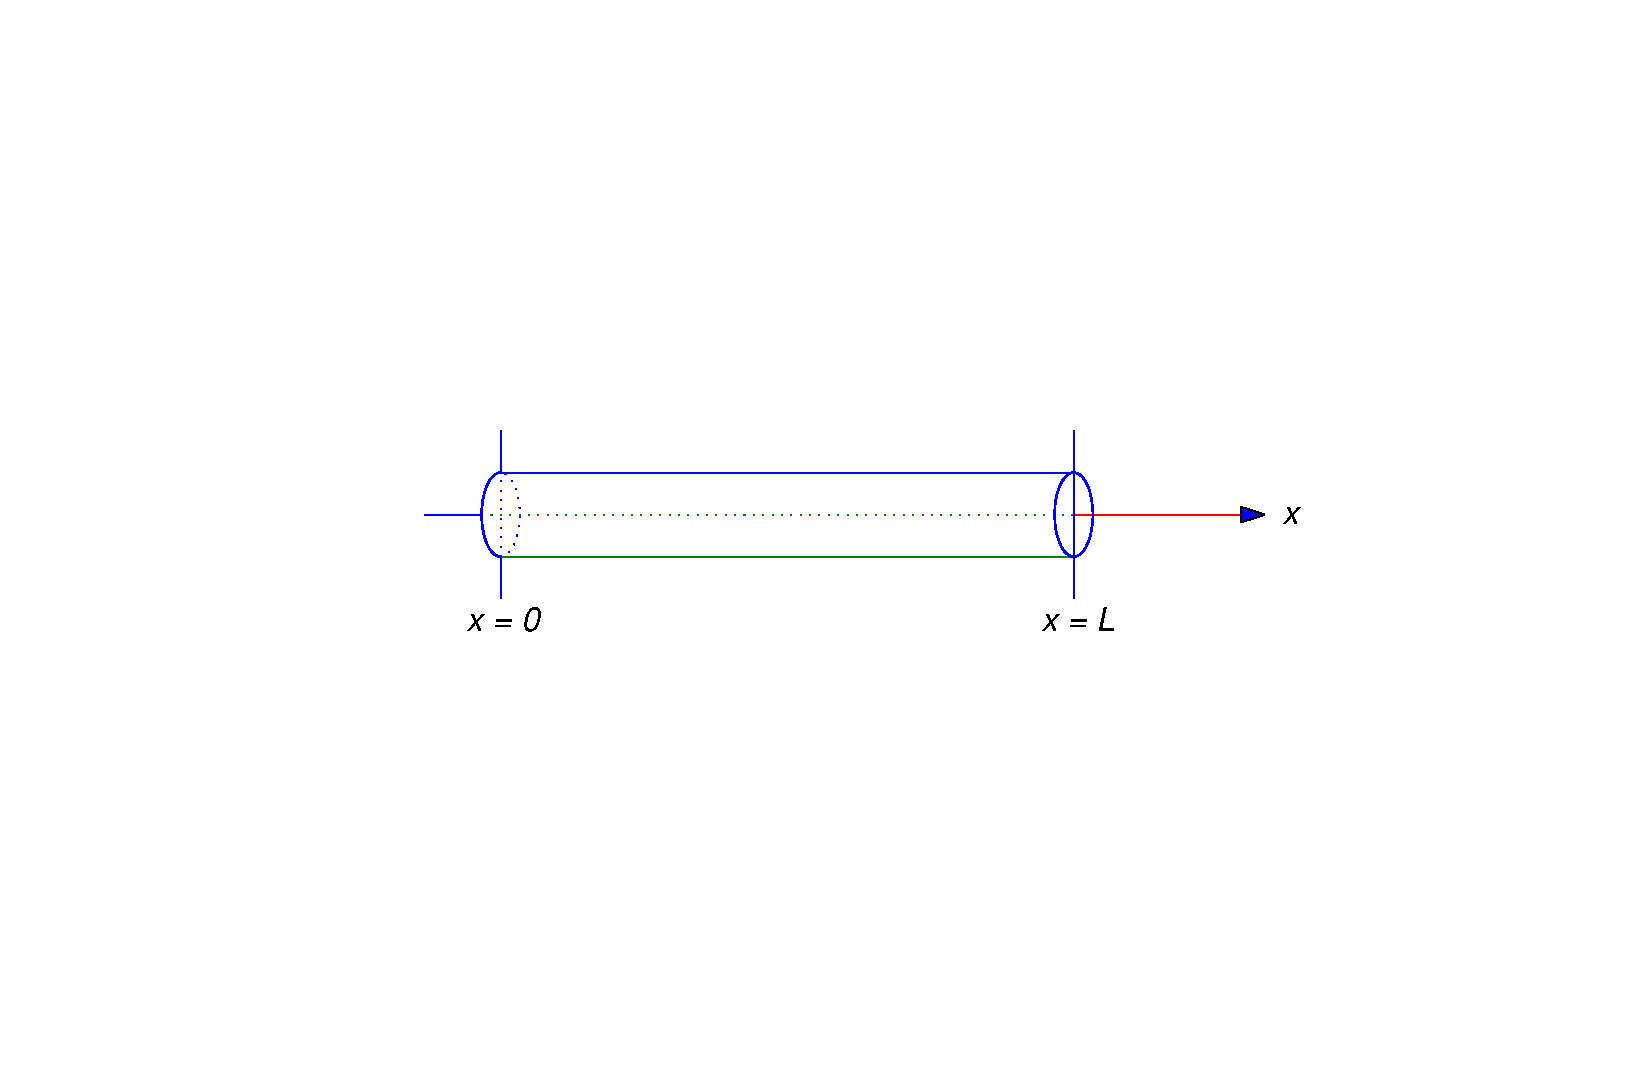
\includegraphics[bb=-78 148 689 643,width=5.67in,height=3.66in,keepaspectratio]{fig120101}
%\caption{A uniform bar of length $L$}
%  \label{figure:12.1.1}
%\end{figure}

We assume that the bar is perfectly insulated except possibly at its endpoints, and that the
temperature is constant on each cross section and therefore depends only on $x$ and $t$. We also
assume that the thermal properties of the bar are independent of $x$ and $t$. In this case, it can
be shown that the temperature $u=u(x,t)$ at time~$t$ at a point $x$ units from the origin satisfies
the partial differential equation
\[
  u_{t}=a^{2}u_{xx},\quad0<x<L,\quad t>0,
\]
where $a$ is a positive constant determined by the thermal properties. This is the {\color{blue}\it
heat equation\/}.

\vspace*{-.2in}
\begin{figure}[H]
  \centering
  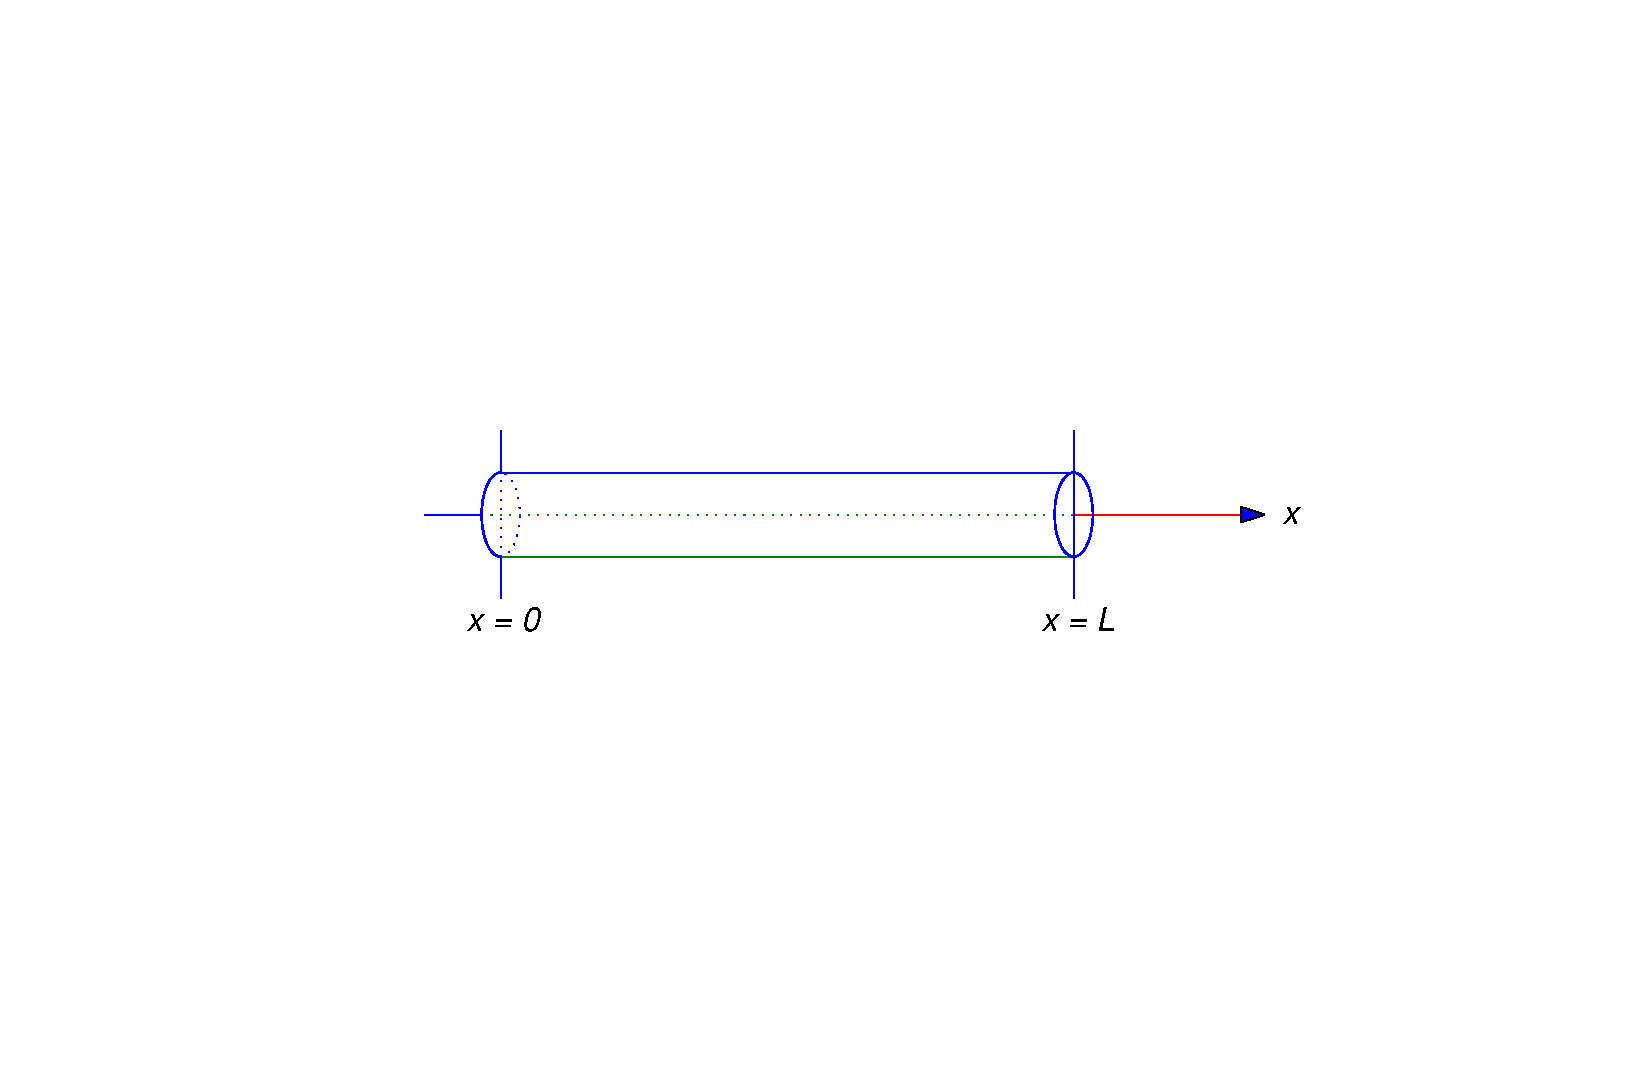
\includegraphics[bb=-78 148 689 643, width=5.67in, height=3.66in, keepaspectratio]{fig120101}
  \vspace*{-1in}
  \caption{A uniform bar of length $L$}
  \label{figure:12.1.1}
\end{figure}

To determine $u$, we must specify the temperature at every point in the bar when $t=0$, say
\[
  u(x,0)=f(x),\quad0\le x\le L.
\]
We call this the {\color{blue}\it initial\/} condition. We must also specify {\color{blue}\it
boundary conditions\/} that $u$ must satisfy at the ends of the bar for all $t>0$. We'll call this
problem an {\color{blue}\it initial-boundary value problem.\/}

We begin with the boundary conditions $u(0,t)=u(L,t)=0$, and write the initial-boundary value
problem as
\begin{equation}
  \label{eq:12.1.1}
  \begin{array}{c}
    u_{t}=a^{2}u_{xx},\quad0<x<L,\quad t>0, \\
    u(0,t)=0,\quad u(L,t)=0,\quad t>0,      \\
    u(x,0)=f(x),\quad0\le x\le L.
  \end{array}
\end{equation}
Our method of solving this problem is called {\color{blue}\it separation of variables\/} (not to be
confused with method of separation of variables used in Section~2.2 for solving ordinary
differential equations). We begin by looking for functions of the form
\[
  v(x,t)=X(x)T(t)
\]
that are not identically zero and satisfy
\[
  v_{t}=a^{2}v_{xx},\quad v(0,t)=0,\quad v(L,t)=0
\]
for all $(x,t)$. Since
\[
  v_{t}=XT'\mbox{\quad and \quad}v_{xx}=X''T,
\]
$v_{t}=a^{2}v_{xx}$ if and only if
\[
  XT'=a^{2}X''T,
\]
which we rewrite as
\[
  \frac{T'}{a^{2}T}=\frac{X''}{X}.
\]
Since the expression on the left is independent of $x$ while the one on the right is independent of
$t$, this equation can hold for all $(x,t)$ only if the two sides equal the same constant, which we
call a {\color{blue}\it separation constant\/}, and write it as $-\lambda$; thus,
\[
  \frac{X''}{X}=\frac{T'}{a^{2}T}=-\lambda.
\]
This is equivalent to
\[
  X''+\lambda X=0
\]
and
\begin{equation}
  \label{eq:12.1.2}T'=-a^{2}\lambda T.
\end{equation}
Since $v(0,t)=X(0)T(t)=0$ and $v(L,t)=X(L)T(t)=0$ and we don't want $T$ to be identically zero,
$X(0)=0$ and $X(L)=0$. Therefore $\lambda$ must be an eigenvalue of the boundary value problem
\begin{equation}
  \label{eq:12.1.3}X''+\lambda X=0,\quad X(0)=0,\quad X(L)=0,
\end{equation}
and $X$ must be a $\lambda$-eigenfunction. From Theorem~\ref{thmtype:11.1.2}, the eigenvalues of
\eqref{eq:12.1.3} are $\lambda_{n}=n^{2}\pi^{2}/L^{2}$, with associated eigenfunctions
\[
  X_{n}=\sin\frac{n\pi x}{L},\quad n=1,2,3,\dots.
\]
Substituting $\lambda=n^{2}\pi^{2}/L^{2}$ into \eqref{eq:12.1.2} yields
\[
  T'=-(n^{2}\pi^{2}a^{2}/L^{2})T,
\]
which has the solution
\[
  T_{n}=e^{-n^{2}\pi^{2}a^{2}t/L^{2}}.
\]
Now let
\[
  v_{n}(x,t)=X_{n}(x)T_{n}(t)=e^{-n^{2}\pi^{2}a^{2}t/L^{2}}\sin\frac{n\pi x}{L},\quad n=1,2,3,\dots
\]
Since
\[
  v_{n}(x,0)=\sin\frac{n\pi x}{L},
\]
$v_{n}$ satisfies \eqref{eq:12.1.1} with $f(x)=\sin n\pi x/L$. More generally, if
$\alpha_{1},\dots,\alpha_{m}$ are constants and
\[
  u_{m}(x,t)= \sum_{n=1}^{m}\alpha_{n}e^{-n^{2}\pi^{2}a^{2}t/L^{2}}\sin\frac{n\pi x}{L},
\]
then $u_{m}$ satisfies \eqref{eq:12.1.1} with
\[
  f(x)=\sum_{n=1}^{m}\alpha_{n}\sin\frac{n\pi x}{L}.
\]
This motivates the next definition.

\begin{definition}
  \color{blue}
  \label{thmtype:12.1.1}\rm The {\color{blue}\it formal solution\/} of the initial-boundary value
  problem
  \begin{equation}
    \label{eq:12.1.4}
    \begin{array}{c}
      u_{t}=a^{2}u_{xx},\quad0<x<L,\quad t>0, \\
      u(0,t)=0,\quad u(L,t)=0,\quad t>0,      \\
      u(x,0)=f(x),\quad0\le x\le L
    \end{array}
  \end{equation}
  is
  \begin{equation}
    \label{eq:12.1.5}u(x,t)=\sum_{n=1}^{\infty}\alpha_{n}e^{-n^{2}\pi^{2}a^{2}t/L^{2}}\sin\frac{n\pi x}{L},
  \end{equation}
  where
  \[
    S(x)=\sum_{n=1}^{\infty}\alpha_{n}\sin\frac{n\pi x}{L}
  \]
  is the Fourier sine series of $f$ on $[0,L]$; that is,
  \[
    \alpha_{n}=\frac{2}{L}\int_{0}^{L}f(x)\sin\frac{n\pi x}{L}\,dx.
  \]
\end{definition}

We use the term ``formal solution'' in this definition because it's not in general true that the
infinite series in \eqref{eq:12.1.5} actually satisfies all the requirements of the initial-boundary
value problem \eqref{eq:12.1.4} when it does, we say that it's an {\color{blue}\it actual
solution\/} of \eqref{eq:12.1.4}.

Because of the negative exponentials in \eqref{eq:12.1.5}, $u$ converges for all $(x,t)$ with $t>0$
(Exercise~\ref{exer:12.1.54}). Since each term in \eqref{eq:12.1.5} satisfies the heat equation and
the boundary conditions in \eqref{eq:12.1.4}, $u$ also has these properties if $u_{t}$ and $u_{xx}$
can be obtained by differentiating the series in \eqref{eq:12.1.5} term by term once with respect to
$t$ and twice with respect to $x$, for $t>0$. However, it's not always legitimate to differentiate
an infinite series term by term. The next theorem gives a useful sufficient condition for legitimacy
of term by term differentiation of an infinite series. We omit the proof.

\begin{theorem}
  \color{blue}
  \label{thmtype:12.1.2} A convergent infinite series
  \[
    W(z)=\sum_{n=1}^{\infty}w_{n}(z)
  \]
  can be differentiated term by term on a closed interval $[z_{1},z_{2}]$ to obtain
  \[
    W'(z)=\sum_{n=1}^{\infty}w_{n}'(z)
  \]
  (where the derivatives at $z=z_{1}$ and $z=z_{2}$ are one-sided) provided that $w_{n}'$ is
  continuous on $[z_{1},z_{2}]$ and
  \[
    |w_{n}'(z)|\le M_{n},\quad z_{1}\le z\le z_{2},\quad n=1,2,3,\dots,
  \]
  where $M_{1}$, $M_{2}$, \dots, $M_{n}$, \dots, are constants such that the series
  $\sum_{n=1}^{\infty}M_{n}$ converges.
\end{theorem}

Theorem~\ref{thmtype:12.1.2}, applied twice with $z=x$ and once with $z=t$, shows that $u_{xx}$ and
$u_{t}$ can be obtained by differentiating $u$ term by term if $t>0$ (Exercise~\ref{exer:12.1.54}).
Therefore $u$ satisfies the heat equation and the boundary conditions in \eqref{eq:12.1.4} for
$t>0$. Therefore, since $u(x,0)=S(x)$ for $0\le x\le L$, $u$ is an actual solution of
\eqref{eq:12.1.4} if and only if $S(x)=f(x)$ for $0\le x\le L$. From Theorem~\ref{thmtype:11.3.2},
this is true if $f$ is continuous and piecewise smooth on $[0,L]$, and $f(0)=f(L)=0$.

In this chapter we'll define formal solutions of several kinds of problems. When we ask you to solve
such problems, we always mean that you should find a formal solution.

\begin{example}
  \label{example:12.1.1} \rm Solve \eqref{eq:12.1.4} with $f(x)=x(x^{2}-3Lx+2L^{2})$.
\end{example}

\solution From Example~\ref{example:11.3.6}, the Fourier sine series of $f$ on $[0,L]$ is
\[
  S(x)=\dst\frac{12L^{3}}{\pi^{3}}\sum_{n=1}^{\infty}\frac{1}{n^{3}}\sin\frac{n\pi x}{L}.
\]
Therefore
\[
  u(x,t)=\dst\frac{12L^{3}}{\pi^{3}}\sum_{n=1}^{\infty}\frac{1}{n^{3}}e^{-n^{2}\pi^{2}a^{2}t/L^{2}}\sin\frac{n\pi x}{L}. \eqno{\bbox}
\]

If both ends of bar are insulated so that no heat can pass through them, then the boundary
conditions are
\[
  u_{x}(0,t)=0,\quad u_{x}(L,t)=0,\quad t>0.
\]
We leave it to you (Exercise~\ref{exer:12.1.1}) to use the method of separation of variables and
Theorem~\ref{thmtype:11.1.3} to motivate the next definition.

\begin{definition}
  \color{blue}
  \label{thmtype:12.1.3} \rm The formal solution of the initial-boundary value problem
  \begin{equation}
    \label{eq:12.1.6}
    \begin{array}{c}
      u_{t}=a^{2}u_{xx},\quad0<x<L,\quad t>0,    \\
      u_{x}(0,t)=0,\quad u_{x}(L,t)=0,\quad t>0, \\
      u(x,0)=f(x),\quad0\le x\le L
    \end{array}
  \end{equation}
  is
  \[
    u(x,t)=\alpha_{0}+\sum_{n=1}^{\infty}\alpha_{n}e^{-n^{2}\pi^{2} a^{2}t/L^{2}}\cos\frac{n\pi x}{L},
  \]
  where
  \[
    C(x)=\alpha_{0}+\sum_{n=1}^{\infty}\alpha_{n}\cos\frac{n\pi x}{L}
  \]
  is the Fourier cosine series of $f$ on $[0,L]$; that is,
  \[
    \alpha_{0}=\frac{1}{L}\int_{0}^{L}f(x)\,dx \mbox{\quad and \quad}\alpha_{n}=\frac{2}{L}\int_{0}^{L}f(x)\cos\frac{n\pi x}{L}\,dx,\quad n=1,2,3,\dots.
  \]
\end{definition}

\begin{example}
  \label{example:12.1.2} \rm Solve \eqref{eq:12.1.6} with $f(x)=x$.
\end{example}

\solution From Example~\ref{example:11.3.1}, the Fourier cosine series of $f$ on $[0,L]$ is
\[
  C(x)=\dst\frac{L}{2}-\frac{4L}{\pi^{2}}\sum_{n=1}^{\infty}\frac{1}{(2n-1)^{2}}\cos\frac{(2n-1)\pi x}{L}.
\]
Therefore
\[
  u(x,t)=\frac{L}{2}-\frac{4L}{\pi^{2}}\sum_{n=1}^{\infty}\frac{1}{(2n-1)^{2}}e^{-(2n-1)^{2}\pi^{2}a^{2}t/L^{2}}\cos\frac{(2n-1)\pi x}{L}. \eqno{\bbox}
\]

We leave it to you (Exercise~\ref{exer:12.1.2}) to use the method of separation of variables and
Theorem~11.1.4 to motivate the next definition.

\begin{definition}
  \color{blue}
  \label{thmtype:12.1.4} \rm The formal solution of the initial-boundary value problem
  \begin{equation}
    \label{eq:12.1.7}
    \begin{array}{c}
      u_{t}=a^{2}u_{xx},\quad0<x<L,\quad t>0, \\
      u(0,t)=0,\quad u_{x}(L,t)=0,\quad t>0,  \\
      u(x,0)=f(x),\quad0\le x\le L
    \end{array}
  \end{equation}
  is
  \[
    u(x,t)=\sum_{n=1}^{\infty}\alpha_{n}e^{-(2n-1)^{2}\pi^{2}a^{2}t/4L^{2}}\sin\frac{(2n-1)\pi x}{2L},
  \]
  where
  \[
    S_{M}(x)=\sum_{n=1}^{\infty}\alpha_{n}\sin\frac{(2n-1)\pi x}{2L}
  \]
  is the mixed Fourier sine series of $f$ on $[0,L]$; that is,
  \[
    \alpha_{n}=\frac{2}{L}\int_{0}^{L}f(x)\sin\frac{(2n-1)\pi x}{2L}\,dx.
  \]
\end{definition}

\begin{example}
  \label{example:12.1.3} \rm Solve \eqref{eq:12.1.7} with $f(x)=x$.
\end{example}

\solution From Example~\ref{example:11.3.4}, the mixed Fourier sine series of $f$ on $[0,L]$ is
\[
  S_{M}(x)=-\frac{8L}{\pi^{2}}\sum_{n=1}^{\infty}\frac{(-1)^{n}}{(2n-1)^{2}}\sin\frac{(2n-1)\pi x}{2L}.
\]
Therefore
\[
  u(x,t)=-\frac{8L}{\pi^{2}}\sum_{n=1}^{\infty}\frac{(-1)^{n}}{(2n-1)^{2}}e^{-(2n-1)^{2}\pi^{2}a^{2}t/4L^{2}}\sin\frac{(2n-1)\pi x}{2L}. \eqno{\bbox}
\]

Figure~\ref{figure:12.1.2} shows a graph of $u=u(x,t)$ plotted with respect to $x$ for various
values of $t$. The line $y=x$ corresponds to $t=0$. The other curves correspond to positive values
of $t$. As $t$ increases, the graphs approach the line $u=0$.

\begin{figure}[tbp]
  \centering
  \color{blue}
  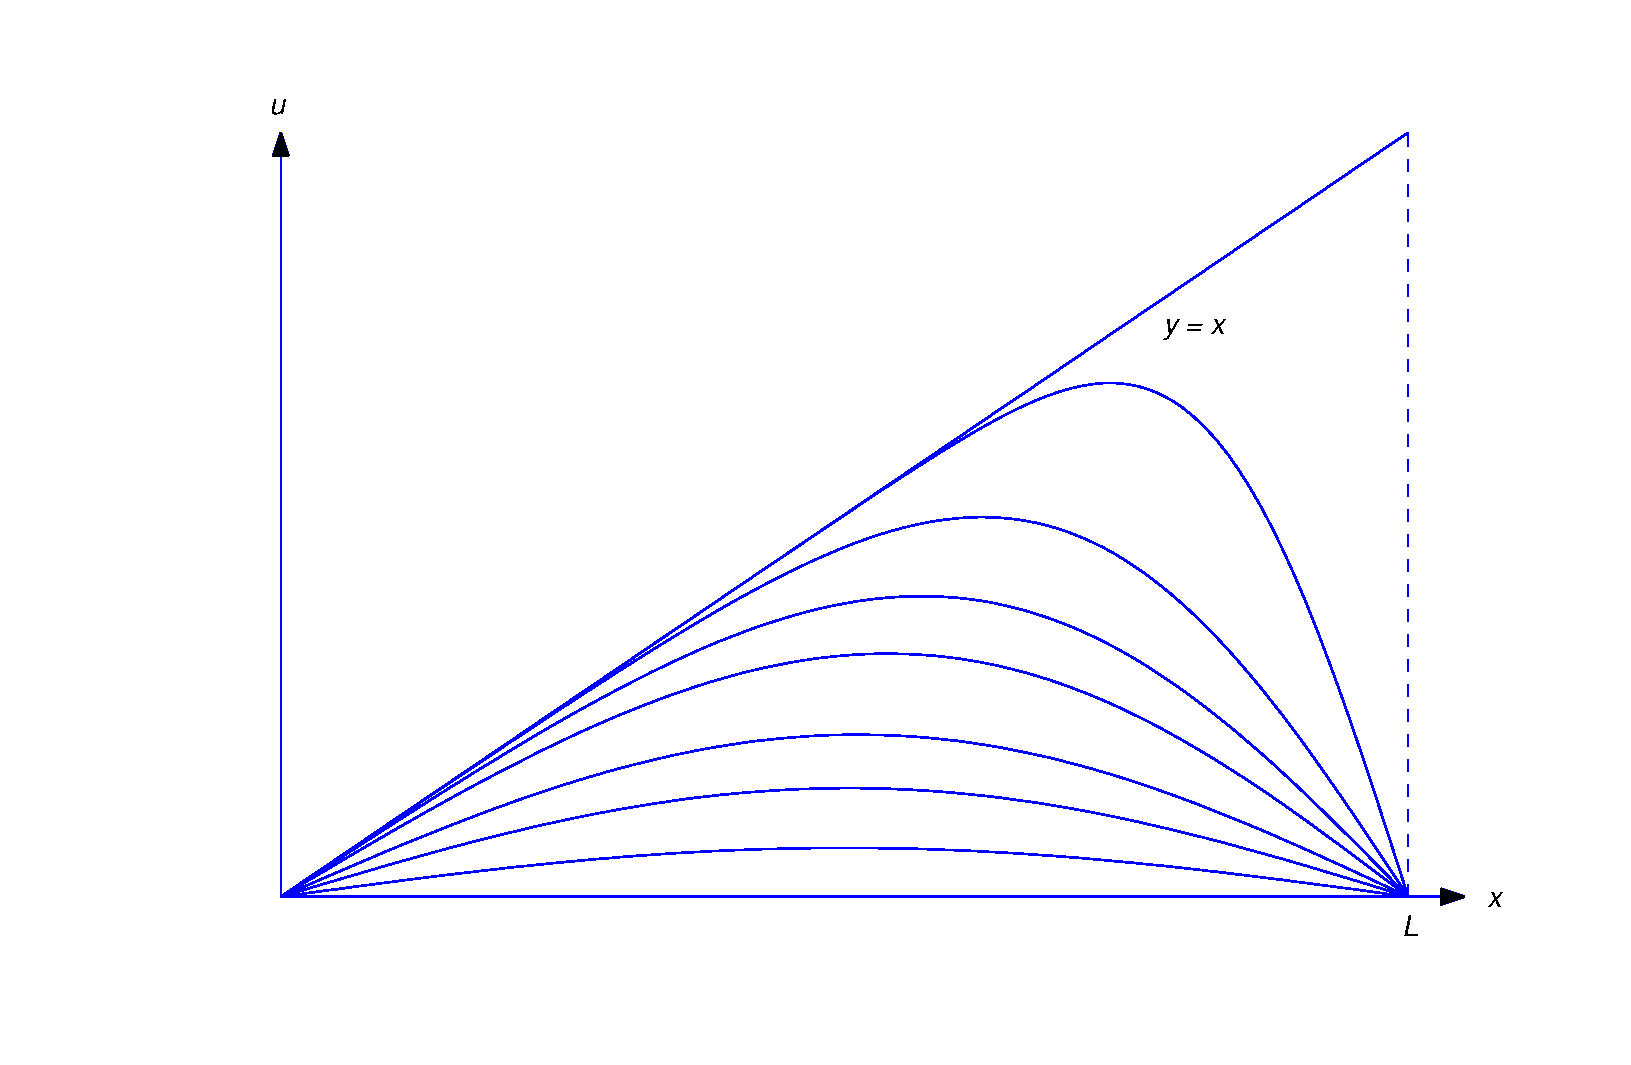
\includegraphics[bb=-78 148 689 643, width=5.67in, height=3.66in, keepaspectratio]{fig120102}
  \caption{}
  \label{figure:12.1.2}
\end{figure}

We leave it to you (Exercise~\ref{exer:12.1.3}) to use the method of separation of variables and
Theorem~\ref{thmtype:11.1.5} to motivate the next definition.

\begin{definition}
  \color{blue}
  \label{thmtype:12.1.5} \rm The formal solution of the initial-boundary value problem
  \begin{equation}
    \label{eq:12.1.8}
    \begin{array}{c}
      u_{t}=a^{2}u_{xx},\quad0<x<L,\quad t>0, \\
      u_{x}(0,t)=0,\quad u(L,t)=0,\quad t>0,  \\
      u(x,0)=f(x),\quad0\le x\le L
    \end{array}
  \end{equation}
  is
  \[
    u(x,t)=\sum_{n=1}^{\infty}\alpha_{n}e^{-(2n-1)^{2}\pi^{2}a^{2}t/4L^{2}}\cos\frac{(2n-1)\pi x}{2L},
  \]
  where
  \[
    C_{M}(x)=\sum_{n=1}^{\infty}\alpha_{n}\cos\frac{(2n-1)\pi x}{2L}
  \]
  is the mixed Fourier cosine series of $f$ on $[0,L]$; that is,
  \[
    \alpha_{n}=\frac{2}{L}\int_{0}^{L}f(x)\cos\frac{(2n-1)\pi x}{2L}\,dx.
  \]
\end{definition}

\begin{example}
  \label{example:12.1.4} \rm Solve \eqref{eq:12.1.8} with $f(x)=x-L$.
\end{example}

\solution From Example~\ref{example:11.3.3}, the mixed Fourier cosine series of $f$ on $[0,L]$ is
\[
  C_{M}(x)=-\frac{8L}{\pi^{2}}\sum_{n=1}^{\infty}\frac{1}{(2n-1)^{2}}\cos\frac{(2n-1)\pi x}{2L}.
\]
Therefore
\[
  u(x,t)=-\frac{8L}{\pi^{2}}\sum_{n=1}^{\infty}\frac{1}{(2n-1)^{2}}e^{-(2n-1)^{2}\pi^{2}a^{2}t/4L^{2}}\cos\frac{(2n-1)\pi x}{2L}.
\]

\boxit{Nonhomogeneous Problems}

\noindent
A problem of the form
\begin{equation}
  \label{eq:12.1.9}
  \begin{array}{c}
    u_{t}=a^{2}u_{xx}+h(x),\quad0<x<L,\quad t>0, \\
    u(0,t)=u_{0},\quad u(L,t)=u_{L},\quad t>0,   \\
    u(x,0)=f(x),\quad0\le x\le L
  \end{array}
\end{equation}
can be transformed to a problem that can be solved by separation of variables. We write
\begin{equation}
  \label{eq:12.1.10}u(x,t)=v(x,t)+q(x),
\end{equation}
where $q$ is to be determined. Then
\[
  u_{t}=v_{t}\mbox{\quad and \quad}u_{xx}=v_{xx}+q''
\]
so $u$ satisfies \eqref{eq:12.1.9} if $v$ satisfies
\[
  \begin{array}{c}
    v_{t}=a^{2}v_{xx}+a^{2}q''(x)+h(x),\quad0<x<L,\quad t>0, \\
    v(0,t)=u_{0}-q(0),\quad v(L,t)=u_{L}-q(L),\quad t>0,     \\
    v(x,0)=f(x)-q(x),\quad0\le x\le L.
  \end{array}
\]
This reduces to
\begin{equation}
  \label{eq:12.1.11}
  \begin{array}{c}
    v_{t}=a^{2}v_{xx},\quad0<x<L,\quad t>0, \\
    v(0,t)=0,\quad v(L,t)=0,\quad t>0,      \\
    v(x,0)=f(x)-q(x),\quad0\le x\le L
  \end{array}
\end{equation}
if
\[
  a^{2}q''+h(x)=0,\quad q(0)=u_{0},\quad q(L)=u_{L}.
\]
We can obtain $q$ by integrating $q''=-h/a^{2}$ twice and choosing the constants of integration so
that $q(0)=u_{0}$ and $q(L)=u_{L}$. Then we can solve \eqref{eq:12.1.11} for $v$ by separation of
variables, and \eqref{eq:12.1.10} is the solution of \eqref{eq:12.1.9}.

\begin{example}
  \label{example:12.1.5} \rm Solve
  \[
    \begin{array}{c}
      u_{t}=u_{xx}-2,\quad0<x<1,\quad t>0,      \\
      u(0,t)=-1,\quad u(1,t)=1,\quad t>0,       \\
      u(x,0)=x^{3}-2x^{2}+3x-1,\quad0\le x\le1.
    \end{array}
  \]

  \solution We leave it to you to show that
  \[
    q(x)=x^{2}+x-1
  \]
  satisfies
  \[
    q''-2=0,\quad q(0)=-1,\quad q(1)=1.
  \]
  Therefore
  \[
    u(x,t)=v(x,t)+x^{2}+x-1,
  \]
  where
  \[
    v_{t}=v_{xx},\quad0<x<1,\quad t>0,
  \]
  \[
    v(0,t)=0,\quad v(1,t)=0,\quad t>0,
  \]
  and
  \[
    v(x,0)=x^{3}-2x^{2}+3x-1-x^{2}-x+1=x(x^{2}-3x+2).
  \]
  From Example~\ref{example:12.1.1} with $a=1$ and $L=1$,
  \[
    v(x,t)= \frac{12}{\pi^{3}}\sum_{n=1}^{\infty}\frac{1}{n^{3}}e^{-n^{2}\pi^{2}t}\sin n\pi x.
  \]
  Therefore
  \[
    u(x,t)=x^{2}+x-1+ \frac{12}{\pi^{3}}\sum_{n=1}^{\infty}\frac{1}{n^{3}}e^{-n^{2}\pi^{2}t}\sin n\pi x. \eqno{\bbox}
  \]
\end{example}

A similar procedure works if the boundary conditions in \eqref{eq:12.1.11} are replaced by mixed
boundary conditions
\[
  u_{x}(0,t)=u_{0},\quad u(L,t)=u_{L},\quad t>0
\]
or
\[
  u(0,t)=u_{0},\quad u_{x}(L,t)=u_{L},\quad t>0;
\]
however, this isn't true in general for the boundary conditions
\[
  u_{x}(0,t)=u_{0},\quad u_{x}(L,t)=u_{L},\quad t>0.
\]
(See Exercise~\ref{exer:12.1.47}.)

\technology
\medskip
Numerical experiments can enhance your understanding of the solutions of initial-boundary value
problems. To be specific, consider the formal solution
\[
  u(x,t)=\sum_{n=1}^{\infty}\alpha_{n}e^{-n^{2}\pi^{2}a^{2}t/L^{2}}\sin\frac{n\pi x}{L},
\]
of \eqref{eq:12.1.4}, where
\[
  S(x)=\sum_{n=1}^{\infty}\alpha_{n}\sin\frac{n\pi x}{L}
\]
is the Fourier sine series of $f$ on $[0,L]$. Consider the $m$-th partial sum
\begin{equation}
  \label{eq:12.1.12}u_{m}(x,t)=\sum_{n=1}^{m}\alpha_{n}e^{-n^{2}\pi^{2}a^{2}t/L^{2}}\sin\frac{n\pi x}{L}.
\end{equation}
For several fixed values of $t$ (including $t=0$), graph $u_{m}(x,t)$ versus $t$. In some cases it
may be useful to graph the curves corresponding to the various values of $t$ on the same axes in
other cases you may want to graph the various curves successively (for increasing values of $t$),
and create a primitive motion picture on your monitor. Repeat this experiment for several values of
$m$, to compare how the results depend upon $m$ for small and large values of $t$. However, keep in
mind that the meanings of ``small'' and ``large'' in this case depend upon the constants $a^{2}$ and
$L^{2}$. A good way to handle this is to rewrite \eqref{eq:12.1.12} as
\[
  u_{m}(x,t)=\sum_{n=1}^{m}\alpha_{n}e^{-n^{2}\tau}\sin\frac{n\pi x}{L},
\]
where
\begin{equation}
  \label{eq:12.1.13}\tau=\frac{\pi^{2}a^{2}t}{L^{2}},
\end{equation}
and graph $u_{m}$ versus $x$ for selected values of $\tau$.

These comments also apply to the situations considered in
Definitions~\ref{thmtype:12.1.3}-\ref{thmtype:12.1.5}, except that \eqref{eq:12.1.13} should be
replaced by
\[
  \tau=\frac{\pi^{2}a^{2}t}{4L^{2}},
\]
in Definitions~\ref{thmtype:12.1.4} and \ref{thmtype:12.1.5}.

In some of the exercises we say ``perform numerical experiments.'' This means that you should
perform the computations just described with the formal solution obtained in the exercise.

\newpage

\exercises
\begin{exerciselist}
  \item\label{exer:12.1.1} Explain Definition~\ref{thmtype:12.1.3}.

  \item\label{exer:12.1.2} Explain Definition~\ref{thmtype:12.1.4}.

  \item\label{exer:12.1.3} Explain Definition~\ref{thmtype:12.1.5}.

  \item\label{exer:12.1.4} \Cex Perform numerical experiments with the formal solution obtained in
        Example~\ref{example:12.1.1}.

  \item\label{exer:12.1.5} \Cex Perform numerical experiments with the formal solution obtained in
        Example~\ref{example:12.1.2}.

  \item\label{exer:12.1.6} \Cex Perform numerical experiments with the formal solution obtained in
        Example~\ref{example:12.1.3}.

  \item\label{exer:12.1.7} \Cex Perform numerical experiments with the formal solution obtained in
        Example~\ref{example:12.1.4}.

  \exercisetext{In Exercises~\ref{exer:12.1.8}-\ref{exer:12.1.42} solve the initial-boundary value
  problem. Where indicated by \Cex, perform numerical experiments. To simplify the computation of
  coefficients in some of these problems, check first to see if $u(x,0)$ is a polynomial that
  satisfies the boundary conditions. If it does, apply Theorem~\ref{thmtype:11.3.5}; also, see
  Exercises~$11.3$.~\hspace*{-3pt}\ref{exer:11.3.35}\part{b},
  $11.3$.~\hspace*{-3pt}\ref{exer:11.3.42}\part{b}, and
  $11.3$.~\hspace*{-3pt}\ref{exer:11.3.50}\part{b}.}

  \item\label{exer:12.1.8} $u_{t}=u_{xx},\quad0<x<1,\quad t>0$,\\ $u(0,t)=0,\quad u(1,t)=0,\quad t>0$,\\ $u(x,0)=x(1-x),\quad0\le x\le1$

  \item\label{exer:12.1.9} $u_{t}=9u_{xx},\quad0<x<4,\quad t>0$,\\ $u(0,t)=0,\quad u(4,t)=0,\quad t>0$,\\ $u(x,0)=1,\quad0\le x\le4$

  \item\label{exer:12.1.10} $u_{t}=3u_{xx},\quad0<x<\pi,\quad t>0$,\\ $u(0,t)=0,\quad u(\pi,t)=0,\quad t>0$,\\ $u(x,0)=x\sin x,\quad0\le x\le\pi$

  \item\label{exer:12.1.11} \Cex $u_{t}=9u_{xx},\quad0<x<2,\quad t>0$,\\ $u(0,t)=0,\quad u(2,t)=0,\quad t>0$,\\ $u(x,0)=x^{2}(2-x),\quad0\le x\le2$

  \item\label{exer:12.1.12} $u_{t}=4u_{xx},\quad0<x<3,\quad t>0$,\\ $u(0,t)=0,\quad u(3,t)=0,\quad t>0$,\\ $u(x,0)=x(9-x^{2}),\quad0\le x\le3$

  \item\label{exer:12.1.13} $u_{t}=4u_{xx},\quad0<x<2,\quad t>0$,\\ $u(0,t)=0,\quad u(2,t)=0,\quad t>0$,\\ $u(x,0)= \left\{
  \begin{array}{cl}
    x,   & 0\le x\le1, \\
    2-x, & 1\le x\le2.
  \end{array}\right.$

  \item\label{exer:12.1.14} $u_{t}=7u_{xx},\quad0<x<1,\quad t>0$,\\ $u(0,t)=0,\quad u(1,t)=0,\quad t>0$,\\ $u(x,0)=x(3x^{4}-10x^{2}+7),\quad0\le x\le1$

  \item\label{exer:12.1.15} $u_{t}=5u_{xx},\quad0<x<1,\quad t>0$,\\ $u(0,t)=0,\quad u(1,t)=0,\quad t>0$,\\ $u(x,0)=x(x^{3}-2x^{2}+1),\quad0\le x\le1$

  \item\label{exer:12.1.16} $u_{t}=2u_{xx},\quad0<x<1,\quad t>0$,\\ $u(0,t)=0,\quad u(1,t)=0,\quad t>0$,\\ $u(x,0)=x(3x^{4}-5x^{3}+2),\quad0\le x\le1$

  \item\label{exer:12.1.17} \Cex $u_{t}=9u_{xx},\quad0<x<4,\quad t>0$,\\ $u_{x}(0,t)=0,\quad u_{x}(4,t)=0,\quad t>0$,\\ $u(x,0)=x^{2},\quad0\le x\le4$

  \item\label{exer:12.1.18} $u_{t}=4u_{xx},\quad0<x<2,\quad t>0$,\\ $u_{x}(0,t)=0,\quad u_{x}(2,t)=0,\quad t>0$,\\ $u(x,0)=x(x-4),\quad0\le x\le2$

  \item\label{exer:12.1.19} \Cex $u_{t}=9u_{xx},\quad0<x<1,\quad t>0$,\\ $u_{x}(0,t)=0,\quad u_{x}(1,t)=0,\quad t>0$,\\ $u(x,0)=x(1-x),\quad0\le x\le1$

  \item\label{exer:12.1.20} $u_{t}=3u_{xx},\quad0<x<2,\quad t>0$,\\ $u_{x}(0,t)=0,\quad u_{x}(2,t)=0,\quad t>0$,\\ $u(x,0)=2x^{2}(3-x),\quad0\le x\le2$

  \item\label{exer:12.1.21} $u_{t}=5u_{xx},\quad0<x<\sqrt{2},\quad t>0$,\\ $u_{x}(0,t)=0,\quad u_{x}(\sqrt{2},t)=0,\quad t>0$,\\ $u(x,0)=3x^{2}(x^{2}-4),\quad0\le x\le\sqrt{2}$

  \item\label{exer:12.1.22} \Cex $u_{t}=3u_{xx},\quad0<x<1,\quad t>0$,\\ $u_{x}(0,t)=0,\quad u_{x}(1,t)=0,\quad t>0$,\\ $u(x,0)=x^{3}(3x-4),\quad0\le x\le1$

  \item\label{exer:12.1.23} $u_{t}=u_{xx},\quad0<x<1,\quad t>0$,\\ $u_{x}(0,t)=0,\quad u_{x}(1,t)=0,\quad t>0$,\\ $u(x,0)=x^{2}(3x^{2}-8x+6),\quad0\le x\le1$

  \item\label{exer:12.1.24} $u_{t}=u_{xx},\quad0<x<\pi,\quad t>0$,\\ $u_{x}(0,t)=0,\quad u_{x}(\pi,t)=0,\quad t>0$,\\ $u(x,0)=x^{2}(x-\pi)^{2},\quad0\le x\le\pi$

  \item\label{exer:12.1.25} $u_{t}=u_{xx},\quad0<x<1,\quad t>0$,\\ $u(0,t)=0,\quad u_{x}(1,t)=0,\quad t>0$,\\ $u(x,0)=\sin\pi x,\quad0\le x\le1$

  \item\label{exer:12.1.26} \Cex $u_{t}=3u_{xx},\quad0<x<\pi,\quad t>0$,\\ $u(0,t)=0,\quad u_{x}(\pi,t)=0,\quad t>0$,\\ $u(x,0)=x(\pi-x),\quad0\le x\le\pi$

  \item\label{exer:12.1.27} $u_{t}=5u_{xx},\quad0<x<2,\quad t>0$,\\ $u(0,t)=0,\quad u_{x}(2,t)=0,\quad t>0$,\\ $u(x,0)=x(4-x),\quad0\le x\le2$

  \item\label{exer:12.1.28} $u_{t}=u_{xx},\quad0<x<1,\quad t>0$,\\ $u(0,t)=0,\quad u_{x}(1,t)=0,\quad t>0$,\\ $u(x,0)=x^{2}(3-2x),\quad0\le x\le1$

  \item\label{exer:12.1.29} $u_{t}=u_{xx},\quad0<x<1,\quad t>0$,\\ $u(0,t)=0,\quad u_{x}(1,t)=0,\quad t>0$,\\ $u(x,0)=(x-1)^{3}+1,\quad0\le x\le1$

  \item\label{exer:12.1.30} \Cex $u_{t}=u_{xx},\quad0<x<1,\quad t>0$,\\ $u(0,t)=0,\quad u_{x}(1,t)=0,\quad t>0$,\\ $u(x,0)=x(x^{2}-3),\quad0\le x\le1$

  \item\label{exer:12.1.31} $u_{t}=u_{xx},\quad0<x<1,\quad t>0$,\\ $u(0,t)=0,\quad u_{x}(1,t)=0,\quad t>0$,\\ $u(x,0)=x^{3}(3x-4),\quad0\le x\le1$

  \item\label{exer:12.1.32} $u_{t}=u_{xx},\quad0<x<1,\quad t>0$,\\ $u(0,t)=0,\quad u_{x}(1,t)=0,\quad t>0$,\\ $u(x,0)=x(x^{3}-2x^{2}+2),\quad0\le x\le1$

  \item\label{exer:12.1.33} $u_{t}=3u_{xx},\quad0<x<\pi,\quad t>0$,\\ $u_{x}(0,t)=0,\quad u(\pi,t)=0,\quad t>0$,\\ $u(x,0)=x^{2}(\pi-x),\quad0\le x\le\pi$

  \item\label{exer:12.1.34} $u_{t}=16u_{xx},\quad0<x<2\pi,\quad t>0$,\\ $u_{x}(0,t)=0,\quad u(2\pi,t)=0,\quad t>0$,\\ $u(x,0)=4,\quad0\le x\le2\pi$

  \item\label{exer:12.1.35} $u_{t}=9u_{xx},\quad0<x<4,\quad t>0$,\\ $u_{x}(0,t)=0,\quad u(4,t)=0,\quad t>0$,\\ $u(x,0)=x^{2},\quad0\le x\le4$

  \item\label{exer:12.1.36} \Cex $u_{t}=3u_{xx},\quad0<x<1,\quad t>0$,\\ $u_{x}(0,t)=0,\quad u(1,t)=0,\quad t>0$,\\ $u(x,0)=1-x,\quad0\le x\le1$

  \item\label{exer:12.1.37} $u_{t}=u_{xx},\quad0<x<1,\quad t>0$,\\ $u_{x}(0,t)=0,\quad u(1,t)=0,\quad t>0$,\\ $u(x,0)=1-x^{3},\quad0\le x\le1$

  \item\label{exer:12.1.38} $u_{t}=7u_{xx},\quad0<x<\pi,\quad t>0$,\\ $u_{x}(0,t)=0,\quad u(\pi,t)=0,\quad t>0$,\\ $u(x,0)=\pi^{2}-x^{2},\quad0\le x\le\pi$

  \item\label{exer:12.1.39} $u_{t}=u_{xx},\quad0<x<1,\quad t>0$,\\ $u_{x}(0,t)=0,\quad u(1,t)=0,\quad t>0$,\\ $u(x,0)=4x^{3}+3x^{2}-7,\quad0\le x\le1$

  \item\label{exer:12.1.40} $u_{t}=u_{xx},\quad0<x<1,\quad t>0$,\\ $u_{x}(0,t)=0,\quad u(1,t)=0,\quad t>0$,\\ $u(x,0)=2x^{3}+3x^{2}-5,\quad0\le x\le1$

  \item\label{exer:12.1.41} \Cex $u_{t}=u_{xx},\quad0<x<1,\quad t>0$,\\ $u_{x}(0,t)=0,\quad u(1,t)=0,\quad t>0$,\\ $u(x,0)=x^{4}-4x^{3}+6x^{2}-3,\quad0\le x\le1$

  \item\label{exer:12.1.42} $u_{t}=u_{xx},\quad0<x<1,\quad t>0$,\\ $u_{x}(0,t)=0,\quad u(1,t)=0,\quad t>0$,\\ $u(x,0)=x^{4}-2x^{3}+1,\quad0\le x\le1$

  \exercisetext{In Exercises~\ref{exer:12.1.43}-\ref{exer:12.1.46} solve the initial-boundary value
  problem. Perform numerical experiments for specific values of $L$ and $a$.}

  \item\label{exer:12.1.43} \Cex $u_{t}=a^{2}u_{xx},\quad0<x<L,\quad t>0$,\\ $u_{x}(0,t)=0,\quad u_{x}(L,t)=0,\quad t>0$,\\ $u(x,0)= \left\{
  \begin{array}{cl}
    1, & 0\le x\le\frac{L}{2}, \\
    0, & \frac{L}{2}<x<L
  \end{array}\right.$

  \item\label{exer:12.1.44} \Cex $u_{t}=a^{2}u_{xx},\quad0<x<L,\quad t>0$,\\ $u(0,t)=0,\quad u(L,t)=0,\quad t>0$,\\ $u(x,0)= \left\{
  \begin{array}{cl}
    1, & 0\le x\le\frac{L}{2}, \\
    0, & \frac{L}{2}<x<L
  \end{array}\right.$

  \item\label{exer:12.1.45} \Cex $u_{t}=a^{2}u_{xx},\quad0<x<L,\quad t>0$,\\ $u_{x}(0,t)=0,\quad u(L,t)=0,\quad t>0$,\\ $u(x,0)= \left\{
  \begin{array}{cl}
    1, & 0\le x\le\frac{L}{2}, \\
    0, & \frac{L}{2}<x<L
  \end{array}\right.$

  \item\label{exer:12.1.46} \Cex $u_{t}=a^{2}u_{xx},\quad0<x<L,\quad t>0$,\\ $u(0,t)=0,\quad u_{x}(L,t)=0,\quad t>0$,\\ $u(x,0)= \left\{
  \begin{array}{cl}
    1, & 0\le x\le\frac{L}{2}, \\
    0, & \frac{L}{2}<x<L
  \end{array}\right.$

  \item\label{exer:12.1.47} Let $h$ be continuous on $[0,L]$ and let $u_{0}$, $u_{L}$, and $a$ be
        constants, with $a>0$. Show that it's always possible to find a function $q$ that satisfies
        \part{a}, \part{b}, or \part{c}, but that this isn't so for \part{d}.
  \begin{alist}
    \item % (a)
    $a^{2}q''+h=0,\quad q(0)=u_{0},\quad q(L)=u_{L}$

    \item % (b)
    $a^{2}q''+h=0,\quad q'(0)=u_{0},\quad q(L)=u_{L}$

    \item % (c)
    $a^{2}q''+h=0,\quad q(0)=u_{0},\quad q'(L)=u_{L}$

    \item % (d)
    $a^{2}q''+h=0,\quad q'(0)=u_{0},\quad q'(L)=u_{L}$
  \end{alist}

  \exercisetext{In Exercises~\ref{exer:12.1.48}-\ref{exer:12.1.53} solve the nonhomogeneous
  initial-boundary value problem}

  \item\label{exer:12.1.48} $u_{t}=9u_{xx}-54x,\quad0<x<4,\quad t>0$,\\ $u(0,t)=1,\quad u(4,t)=61,\quad t>0$,\\ $u(x,0)=2-x+x^{3},\quad0\le x\le4$

  \item\label{exer:12.1.49} $u_{t}=u_{xx}-2,\quad0<x<1,\quad t>0$,\\ $u(0,t)=1,\quad u(1,t)=3,\quad t>0$,\\ $u(x,0)=2x^{2}+1,\quad0\le x\le1$

  \item\label{exer:12.1.50} $u_{t}=3u_{xx}-18x,\quad0<x<1,\quad t>0$,\\ $u_{x}(0,t)=-1,\quad u(1,t)=-1,\quad t>0$,\\ $u(x,0)=x^{3}-2x,\quad0\le x\le1$

  \item\label{exer:12.1.51} $u_{t}=9u_{xx}-18,\quad0<x<4,\quad t>0$,\\ $u_{x}(0,t)=-1,\quad u(4,t)=10,\quad t>0$,\\ $u(x,0)=2x^{2}-x-2,\quad0\le x\le4$

  \item\label{exer:12.1.52} $u_{t}=u_{xx}+\pi^{2}\sin\pi x,\quad0<x<1,\quad t>0$,\\ $u(0,t)=0,\quad u_{x}(1,t)=-\pi,\quad t>0$,\\ $u(x,0)=2\sin\pi x,\quad0\le x\le1$

  \item\label{exer:12.1.53} $u_{t}=u_{xx}-6x,\quad0<x<L,\quad t>0$,\\ $u(0,t)=3,\quad u_{x}(1,t)=2,\quad t>0$,\\ $u(x,0)=x^{3}-x^{2}+x+3,\quad0\le x\le1$

  \item\label{exer:12.1.54} In this exercise take it as given that the infinite series
        $\sum_{n=1}^{\infty}n^{p}e^{-qn^{2}}$ converges for all $p$ if $q>0$, and, where
        appropriate, use the comparison test for absolute convergence of an infinite series.

  Let
  \[
    u(x,t)=\sum_{n=1}^{\infty}\alpha_{n}e^{-n^{2}\pi^{2} a^{2}t/L^{2}}\sin\frac{n\pi x}{L}
  \]
  where
  \[
    \alpha_{n}=\frac{2}{L}\int_{0}^{L}f(x)\sin\frac{n\pi x}{L}\,dx
  \]
  and $f$ is piecewise smooth on $[0,L]$.

  \begin{alist}
    \item % (a)
    Show that $u$ is defined for $(x,t)$ such that $t>0$.

    \item % (b)
    For fixed $t>0$, use Theorem~\ref{thmtype:12.1.2} with $z=x$ to show that
    \[
      u_{x}(x,t)=\frac{\pi}{L}\sum_{n=1}^{\infty}n\alpha_{n}e^{-n^{2}\pi^{2} a^{2}t/L^{2}}\cos\frac{n\pi x}{L},\quad-\infty<x<\infty.
    \]

    \item % (c)
    Starting from the result of \part{a}, use Theorem~\ref{thmtype:12.1.2} with $z=x$ to show that,
    for a fixed $t>0$,
    \[
      u_{xx}(x,t)=-\frac{\pi^{2}}{L^{2}}\sum_{n=1}^{\infty}n^{2}\alpha_{n}e^{-n^{2}\pi^{2}a^{2}t/L^{2}}\sin\frac{n\pi x}{L},\quad-\infty<x<\infty.
    \]

    \item % (d)
    For fixed but arbitrary $x$, use Theorem~\ref{thmtype:12.1.2} with $z=t$ to show that
    \[
      u_{t}(x,t)=-\frac{\pi^{2}a^{2}}{L^{2}}\sum_{n=1}^{\infty}n^{2}\alpha_{n}e^{-n^{2}\pi^{2}a^{2}t/L^{2}}\sin\frac{n\pi x}{L},
    \]
    if $t>t_{0}>0$, where $t_{0}$ is an arbitrary positive number. Then argue that since $t_{0}$ is
    arbitrary, the conclusion holds for all $t>0$.

    \item % (e)
    Conclude from \part{c} and \part{d} that
    \[
      u_{t}=a^{2}u_{xx},\quad-\infty<x<\infty,\quad t>0.
    \]
  \end{alist}

  By repeatedly applying the arguments in \part{a} and \part{c}, it can be shown that $u$ can be
  differentiated term by term any number of times with respect to $x$ and/or $t$ if $t>0$.
\end{exerciselist}


\section{The Wave Equation}

\noindent
In this section we consider initial-boundary value problems of the
form
\begin{equation} \label{eq:12.2.1}
\begin{array}{c}
u_{tt}=a^2u_{xx},\quad 0<x<L,\quad t>0,\\
u(0,t)=0,\quad u(L,t)=0,\quad t>0,\\
u(x,0)=f(x),\quad u_t(x,0)=g(x), \quad 0\le x\le L,
\end{array}
\end{equation}
where $a$ is a constant and $f$ and $g$  are given functions of $x$.

The partial differential equation $u_{tt}=a^2u_{xx}$  is called the
{\color{blue}\it wave equation\/}. It is necessary to specify both $f$ and $g$
because the wave equation is a second order equation in $t$
for each fixed $x$.

 This equation and its generalizations
$$
u_{tt}=a^2(u_{xx}+u_{yy})\mbox{\quad and \quad}
u_{tt}=a^2(u_{xx}+u_{yy}+u_{zz})
$$
to two and three space dimensions have important applications to the propagation of electromagnetic, sonic, and water
waves.

\boxit{The Vibrating String}

\noindent
 We  motivate the study of the  wave
equation by considering its application to the vibrations of a string
 -- such as a violin string --
tightly stretched in equilibrium along the $x$-axis in the $xu$-plane
and tied to the points $(0,0)$ and $(L,0)$ (Figure~\ref{figure:12.2.1}).

\begin{figure}[tbp]
  \centering\color{blue}
  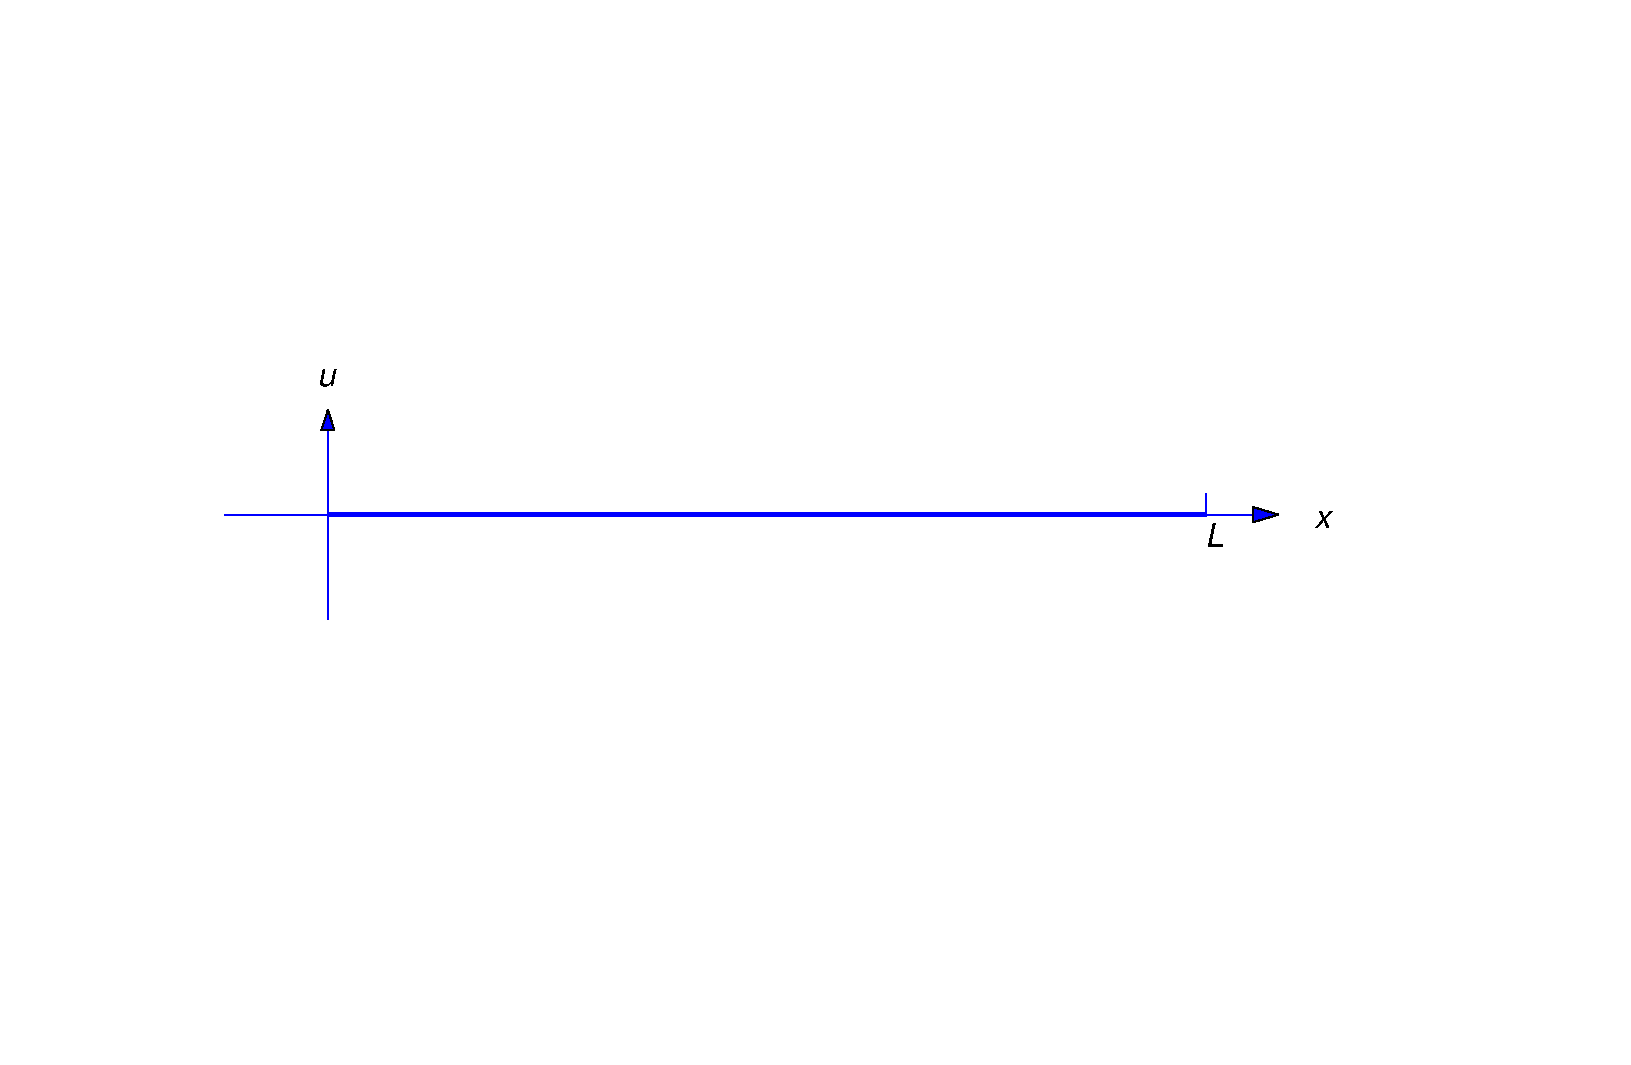
\includegraphics[bb=-78 148 689 643,width=5.67in,height=3.66in,keepaspectratio]{fig120201}
\caption{A stretched string}
  \label{figure:12.2.1}
\end{figure}

If the string is plucked in the vertical direction and released at
time $t=0$, it will oscillate in the $xu$-plane.
Let $u(x,t)$ denote
the displacement of the point on the string above (or below) the
abscissa $x$ at time $t$.

We'll show that it's reasonable to assume that $u$ satisfies the
wave equation under the following assumptions:

\begin{numberlist}
\item % (1)
The mass density (mass per unit length) $\rho$ of the string is
constant throughout the string.
\item % (2)
The tension $T$ induced by tightly stretching the string along the
$x$-axis is so great that all other forces, such as gravity and air
resistance, can be neglected.
\item % (3)
The tension at any point on the
string acts along the tangent to the string at that point,
and the magnitude of its horizontal  component
is always equal to $T$, the tension in the string in equilibrium.
\item % (4)
The slope of the string at every point remains sufficiently small
so that we can make the
approximation
\begin{equation} \label{eq:12.2.2}
\sqrt{1+u_x^2}\approx1.
\end{equation}
\end{numberlist}

Figure~\ref{figure:12.2.2} shows a segment of the displaced string
at a time $t>0$.  (Don't think that the figure  is
necessarily inconsistent
with Assumption~4;     we exaggerated the slope for clarity.)

\begin{figure}[tbp]
  \centering\color{blue}
  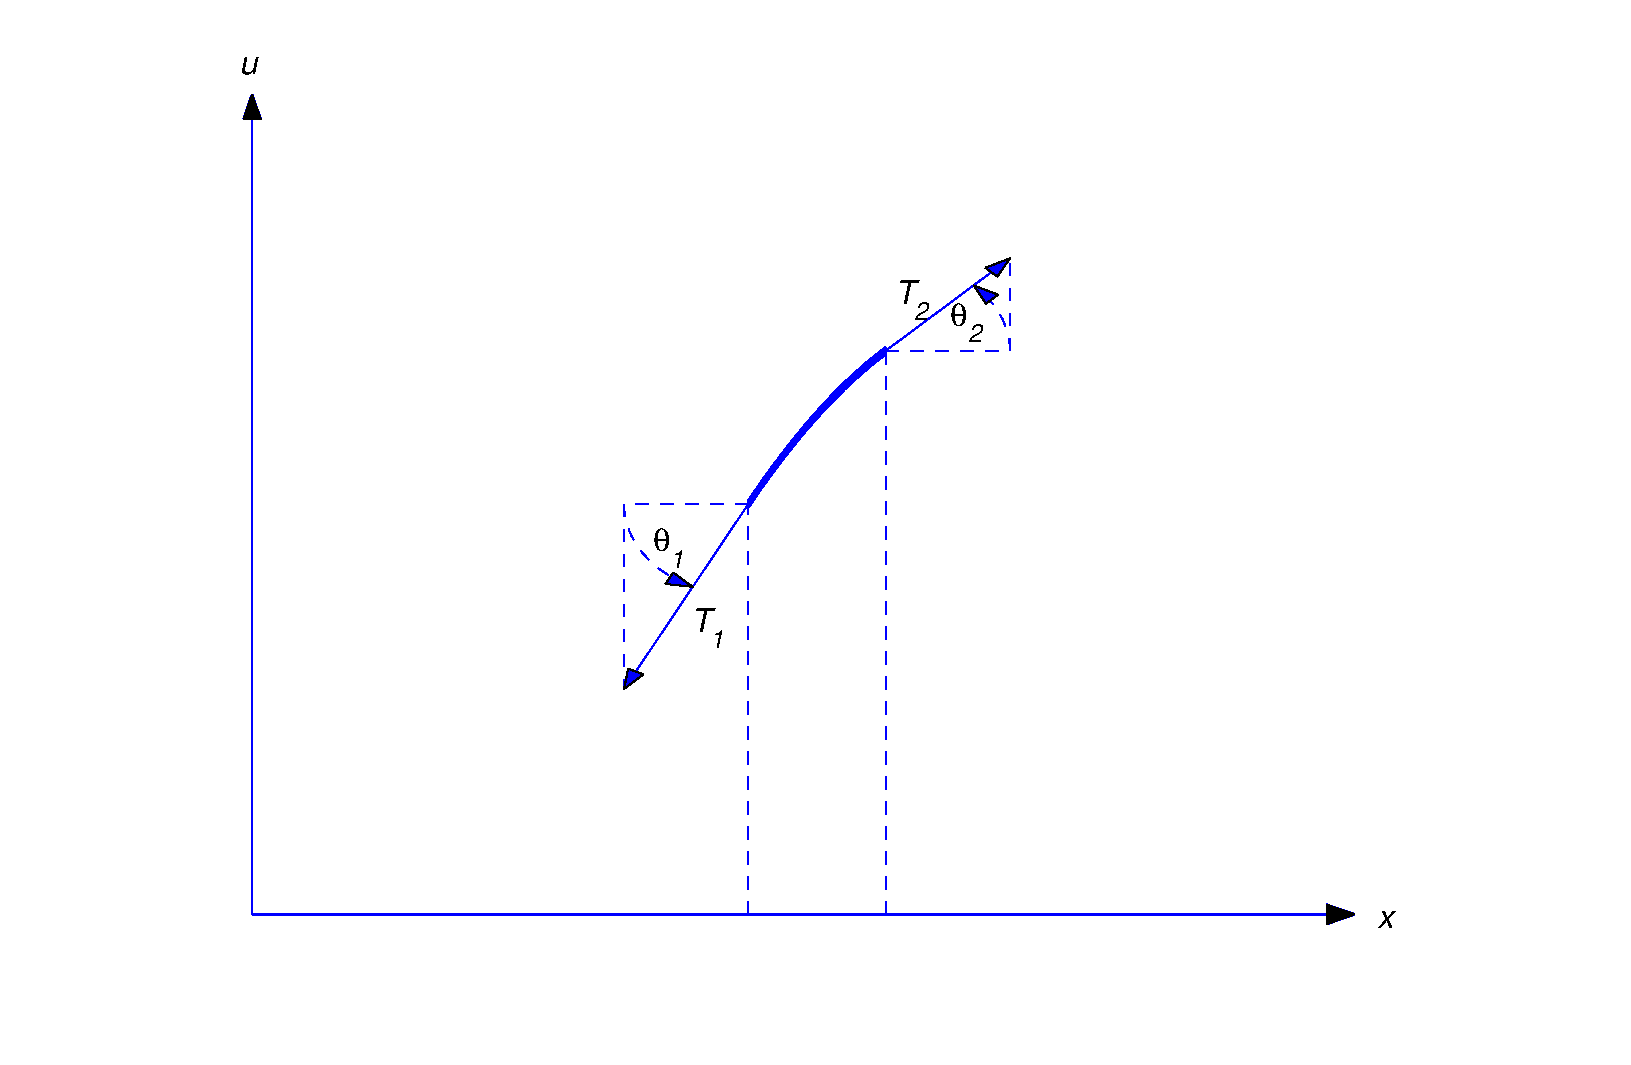
\includegraphics[bb=-78 148 689 643,width=5.67in,height=3.66in,keepaspectratio]{fig120202}
\caption{ A segment of the displaced string}
  \label{figure:12.2.2}
\end{figure}

 The vectors ${\bf T}_1$ and ${\bf T}_2$ are the forces
due to tension, acting along the tangents to the segment at its
endpoints.
From Newton's second law of motion, ${\bf T}_1-{\bf T}_2$
is equal to the mass times the acceleration of the center of
mass of the segment.
The horizontal and vertical components of ${\bf T}_1-{\bf T}_2$
 are
$$
|{\bf T}_2|\cos\theta_2- |{\bf T}_1|\cos\theta_1
\mbox{\quad and \quad}
|{\bf T}_2|\sin\theta_2- |{\bf T}_1|\sin\theta_1,
$$
respectively.
Since
\begin{equation} \label{eq:12.2.3}
|{\bf T}_2|\cos\theta_2=|{\bf T}_1|\cos\theta_1=T
\end{equation}
by assumption, the net horizontal force is zero, so there's
no horizontal acceleration. Since the initial horizontal
velocity is zero, there's no horizontal motion.

Applying Newton's second law of motion in the  vertical direction
yields
\begin{equation} \label{eq:12.2.4}
|{\bf T}_2|\sin\theta_2- |{\bf T}_1|\sin\theta_1=\rho\Delta
s\,u_{tt}(\overline x,t),
\end{equation}
where $\Delta s$ is the length of the segment  and $\overline x$
is the abscissa of the center of mass; hence,
$$
x<\overline x<x+\Delta x.
$$
From calculus, we know that
$$
\Delta s=\int_x^{x+\Delta x}\sqrt{1+u_x^2(\sigma,t)}\,d\sigma;
$$
however, because of \eqref{eq:12.2.2}, we make the approximation
$$
\Delta s\approx\int_x^{x+\Delta x}1\,d\sigma=\Delta x,
$$
so \eqref{eq:12.2.4} becomes
$$
|{\bf T}_2|\sin\theta_2- |{\bf T}_1|\sin\theta_1=\rho\Delta
x\,u_{tt}(\overline x,t).
$$
Therefore
$$
{|{\bf T}_2|\sin\theta_2- |{\bf T}_1|\sin\theta_1\over\Delta x}=\rho
u_{tt}(\overline x,t).
$$
Recalling \eqref{eq:12.2.3}, we divide  by $T$    to obtain
\begin{equation} \label{eq:12.2.5}
{\tan\theta_2-\tan\theta_1\over\Delta x}=
{\rho\over T}u_{tt}(\overline x,t).
\end{equation}
Since
$\tan\theta_1=u_x(x,t)$ and $\tan\theta_2=u_x(x+\Delta x,t)$,
\eqref{eq:12.2.5} is equivalent to
$$
{u_x(x+\Delta x)-u_x(x,t)\over \Delta x}=
{\rho\over T}u_{tt}(\overline x,t).
$$
Letting $\Delta x\to 0$  yields
$$
u_{xx}(x,t)={\rho\over T}u_{tt}(x,t),
$$
which we rewrite as $u_{tt}=a^2u_{xx}$, with $a^2=T/\rho$.

\boxit{The Formal Solution}

\noindent
As in Section~12.1, we use
 separation
of variables to obtain a suitable definition for the formal solution
of \eqref{eq:12.2.1}.
 We begin by looking for functions of the form
$v(x,t)=X(x)T(t)$
that are not identically zero and satisfy
$$
v_{tt}=a^2v_{xx},\quad
v(0,t)=0,\quad v(L,t)=0
$$
for all $(x,t)$.
Since
$$
v_{tt}=XT''\mbox{\quad and \quad}v_{xx}=X''T,
$$
$v_{tt}=a^2v_{xx}$ if and only if
$$
XT''=a^2X''T,
$$
which we rewrite as
$$
{T''\over a^2T}={X''\over X}.
$$
For this  to hold for all $(x,t)$,
 the two sides must equal the same constant;
thus,
$$
{X''\over X}={T''\over a^2T}=-\lambda,
$$
which is equivalent to
$$
X''+\lambda X=0
$$
and
\begin{equation} \label{eq:12.2.6}
T''+a^2\lambda T=0.
\end{equation}
Since $v(0,t)=X(0)T(t)=0$ and $v(L,t)=X(L)T(t)=0$ and we don't want
$T$ to be  identically
zero,  $X(0)=0$ and $X(L)=0$. Therefore $\lambda$
must be an eigenvalue of
\begin{equation} \label{eq:12.2.7}
X''+\lambda X=0,\quad X(0)=0,\quad X(L)=0,
\end{equation}
and $X$ must be a $\lambda$-eigenfunction.
 From Theorem~\ref{thmtype:11.1.2}, the eigenvalues of \eqref{eq:12.2.7}
are $\lambda_n=n^2\pi^2/L^2$, with
associated eigenfunctions
$$
X_n=\sin{n\pi x\over L}, \quad n=1,2,3,\dots.
$$
Substituting $\lambda=n^2\pi^2/L^2$  into
\eqref{eq:12.2.6} yields
$$
T''+(n^2\pi^2a^2/L^2)T=0,
$$
which has the general solution
$$
T_n=\alpha_n\cos{n\pi at\over L}+{\beta_nL\over n\pi a}\sin{n\pi
at\over L},
$$
where $\alpha_n$  and $\beta_n$ are constants. Now let
$$
v_n(x,t)=X_n(x)T_n(t)=\left(\alpha_n\cos{n\pi at\over L}+
{\beta_nL\over n\pi a}\sin{n\pi at\over L}\right)
\sin{n\pi x\over L}.
$$
Then
$$
{\partial v_n\over\partial t}(x,t)=
\left(-{n\pi a \over L}\alpha_n\sin{n\pi at\over L}
+\beta_n\cos{n\pi at\over L}\right)\sin{n\pi x\over L},
$$
so
$$
v_n(x,0)=\alpha_n\sin{n\pi x\over L}
\mbox{\quad and \quad}
{\partial v_n\over\partial t}(x,0)=\beta_n
\sin{n\pi x\over L}.
$$
Therefore $v_n$ satisfies \eqref{eq:12.2.1} with
$f(x)=\alpha_n \sin n\pi x/L$ and  $g(x)=\beta_n\cos n\pi x/L$.
More generally, if $\alpha_1$,  $\alpha_2$, \dots, $\alpha_m$
and $\beta_1$, $\beta_2$,\dots, $\beta_m$ are constants and
$$
u_m(x,t)=\sum_{n=1}^m\left(\alpha_n\cos{n\pi at\over
L}+{\beta_nL\over n\pi a}\sin{n\pi at\over L}\right)
\sin{n\pi x\over L},
$$
then $u_m$ satisfies \eqref{eq:12.2.1} with
$$
f(x)=\sum_{n=1}^m \alpha_n\sin{n\pi x\over L}
\mbox{\quad and \quad}
g(x)=\sum_{n=1}^m \beta_n\sin{n\pi x\over L}.
$$
 This motivates the next definition.

\begin{definition}\color{blue} \label{thmtype:12.2.1}\rm
If $f$ and $g$ are piecewise smooth of $[0,L]$, then
the  formal solution of  \eqref{eq:12.2.1}
is
\begin{equation} \label{eq:12.2.8}
u(x,t)=\sum_{n=1}^\infty\left(\alpha_n\cos{n\pi at\over
L}+{\beta_nL\over n\pi a}\sin{n\pi at\over L}\right)
\sin{n\pi x\over L},
\end{equation}
where
$$
S_f(x)=\sum_{n=1}^\infty \alpha_n\sin{n\pi x\over L}
\mbox{\quad and \quad}
S_{g}(x)=\sum_{n=1}^\infty \beta_n\sin{n\pi x\over L}
$$
are the   Fourier sine series of $f$ and $g$ on $[0,L]$; that is,
$$
\alpha_n={2\over L}\int_0^Lf(x)\sin{n\pi x\over L}\,dx
\mbox{\quad and \quad}
\beta_n={2\over L}\int_0^Lg(x)\sin{n\pi x\over L}\,dx.
$$
\end{definition}

Since there are no  convergence-producing factors in \eqref{eq:12.2.8}
like the negative exponentials in $t$ that appear in formal solutions
of initial-boundary value problems for the heat equation, it isn't
obvious that  \eqref{eq:12.2.8} even converges
for any values of $x$ and $t$, let alone that it can be differentiated
term by term  to show that $u_{tt}=a^2u_{xx}$.
However, the next
theorem guarantees that  the series  converges
not only for $0\le x\le L$  and $t\ge0$, but for $-\infty<x<\infty$
and $-\infty<t<\infty$.

\begin{theorem}\color{blue} \label{thmtype:12.2.2}
If $f$ and $g$ are piecewise smooth on $[0,L]$, then
$u$ in \eqref{eq:12.2.1} converges for all $(x,t)$,
and can be written as
\begin{equation} \label{eq:12.2.9}
u(x,t)={1\over2}[S_f(x+at)+S_f(x-at)]+
{1\over2a}\int_{x-at}^{x+at}S_g(\tau)\,d\tau.
\end{equation}
\end{theorem}

\proof
Setting $A=n\pi x/L$ and $B=n\pi at/L$ in the  identities
$$
\sin A\cos B=\phantom{-}{1\over2}[\sin(A+B)+\sin(A-B)]
$$
and
$$
\sin A\sin B=-{1\over2}[\cos(A+B)-\cos(A-B)]
$$
yields
\begin{equation} \label{eq:12.2.10}
\cos{n\pi at\over L}\sin{n\pi x\over L}
={1\over2}\left[\sin{n\pi(x+at)\over
L}+\sin{n\pi(x-at)\over L}\right]
\end{equation}
and
\begin{equation} \label{eq:12.2.11}
\begin{array}{rcl}
\dst \sin{n\pi at\over L}\sin{n\pi x\over L}
&=&-\dst{1\over2}\left[\cos{n\pi(x+at)\over
L}-\cos{n\pi(x-at)\over
L}\right]\\&=&\dst{n\pi\over2L}\int_{x-at}^{x+at}
\sin{n\pi\tau\over L}\,d\tau.
\end{array}
\end{equation}
From  \eqref{eq:12.2.10},
\begin{equation} \label{eq:12.2.12}
\begin{array}{rcl}
\dst\sum_{n=1}^\infty\alpha_n \cos{n\pi at\over L}\sin{n\pi x\over
L}&=&
\dst{1\over2}\sum_{n=1}^\infty\alpha_n\left(\sin{n\pi(x+at)\over
L}
+\sin{n\pi(x-at)\over L}\right)\\
&=&\dst{1\over2}[S_f(x+at)+S_f(x-at)].
\end{array}
\end{equation}
Since it can be shown that a Fourier sine series can be integrated
term by term between any two limits,
\eqref{eq:12.2.11} implies that
$$
\begin{array}{rcl}
\dst\sum_{n=1}^\infty{\beta_nL\over n\pi a}
\sin{n\pi at\over L}\sin{n\pi x\over L}&=&
\dst{1\over2a}\sum_{n=1}^\infty \beta_n\int_{x-at}^{x+at}
\sin{n\pi\tau\over L}\,d\tau\\
&=&\dst{1\over2a}\int_{x-at}^{x+at}\left(\sum_{n=1}^\infty \beta_n
\sin{n\pi\tau\over L}\right)\,d\tau\\
&=&
\dst{1\over2a}\int_{x-at}^{x+at}S_g(\tau)\,d\tau.
\end{array}
$$
This and  \eqref{eq:12.2.12} imply \eqref{eq:12.2.9},
which completes the proof.

As we'll see below, if $S_g$ is differentiable and $S_f$
is twice differentiable on $(-\infty,\infty)$, then
\eqref{eq:12.2.9} satisfies $u_{tt}=a^2u_{xx}$ for all $(x,t)$. We need the
next theorem to formulate conditions on $f$ and $g$ such that
$S_f$ and $S_g$ to have these properties.

\begin{theorem}\color{blue} \label{thmtype:12.2.3}
Suppose $h$ is differentiable on $[0,L]$; that is,
$h'(x)$ exists for $0<x<L$, and the one-sided derivatives
$$
h'_+(0)=\lim_{x\to0+}{h(x)-h(0)\over x}
\mbox{\quad and \quad}
h'_-(L)=\lim_{x\to L-}{h(x)-h(L)\over x-L}
$$
both exist.

\part{a}
Let $p$ be the odd periodic extension of $h$ to $(-\infty,\infty)$;
that is,
$$
p(x)=
\left\{\begin{array}{cl}
h(x),&\quad 0\le x\le L,\\
-h(-x),&-L<x<0,
\end{array}\right.
\mbox{\  and\  } p(x+2L)=p(x),\quad -\infty<x<\infty.
$$
Then $p$ is differentiable on $(-\infty,\infty)$ if and only
if
\begin{equation} \label{eq:12.2.13}
h(0)=h(L)=0.
\end{equation}

\part{b}
Let $q$ be the even periodic extension of $h$ to $(-\infty,\infty)$;
that is,
$$
q(x)=
\left\{\begin{array}{cl}
h(x),&\quad 0\le x\le L,\\
h(-x),&-L<x<0,
\end{array}\right.
\mbox{\  and\  } q(x+2L)=q(x),\quad -\infty<x<\infty.
$$
Then $q$ is differentiable on $(-\infty,\infty)$ if and only
if
\begin{equation} \label{eq:12.2.14}
h'_+(0)=h'_-(L)=0.
\end{equation}
\end{theorem}

\proof
Throughout this proof, $k$ denotes an integer.
Since $f$ is differentiable on the open interval
$(0,L)$, both $p$ and $q$ are differentiable on every
open interval $((k-1)L,kL)$. Thus, we need
only to  determine whether $p$ and $q$ are differentiable
at $x=kL$ for every  $k$.

\part{a}
From Figure~\ref{figure:12.2.3},
 $p$ is discontinuous at $x=2kL$ if $h(0)\ne0$
and   discontinuous at $x=(2k-1)L$ if $h(L)\ne0$.
Therefore $p$
is not differentiable on $(-\infty,\infty)$  unless $h(0)=h(L)=0$.
From
 Figure~\ref{figure:12.2.4}, if $h(0)=h(L)=0$, then
$$
p'(2kL)=h_+'(0)\mbox{\quad and \quad}p'((2k-1)L)=h_-'(L)
$$
for every  $k$;  therefore, $p$ is differentiable on
$(-\infty,\infty)$.

\begin{figure}[htbp]
\color{blue}
  \begin{minipage}[b]{0.5\linewidth}
    \centering
   \scalebox{.55}{
  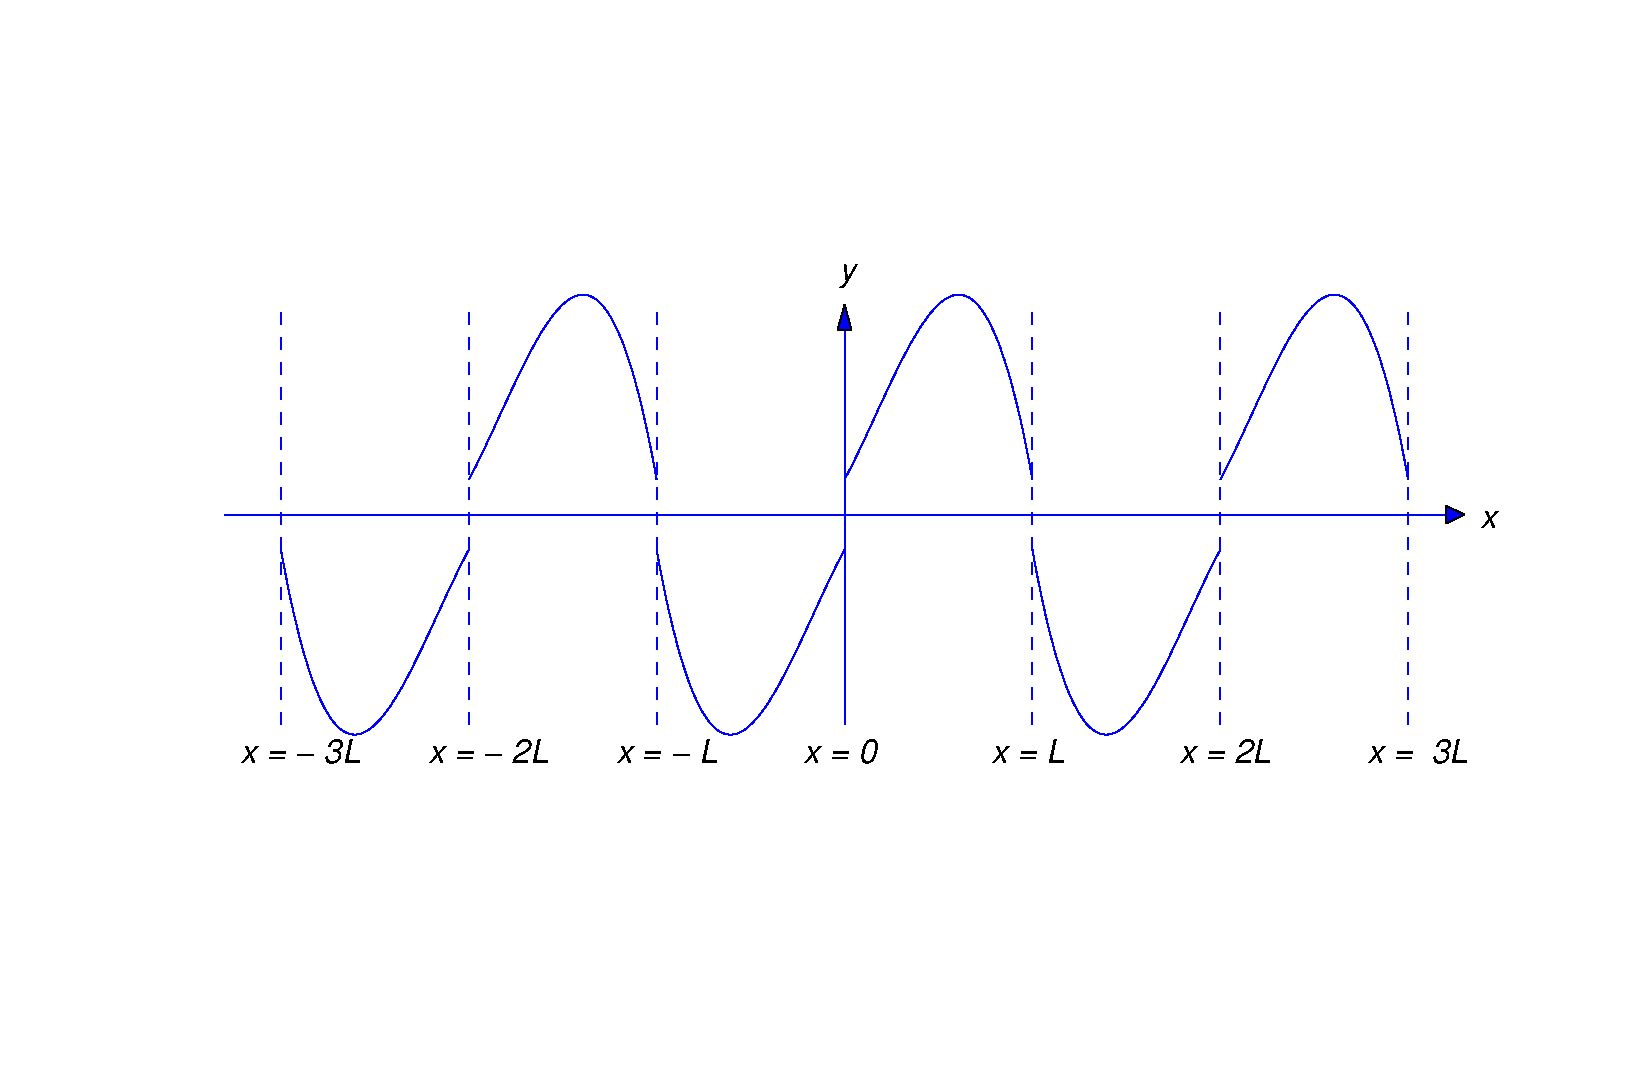
\includegraphics[bb=-78 148 689 643,width=5.67in,height=3.66in,keepaspectratio]{fig120203}}
\caption{ The odd extension of a function that does
not satisfy \eqref{eq:12.2.13}}
  \label{figure:12.2.3}
\end{minipage}
  \begin{minipage}[b]{0.5\linewidth}
    \centering
   \scalebox{.55}{
  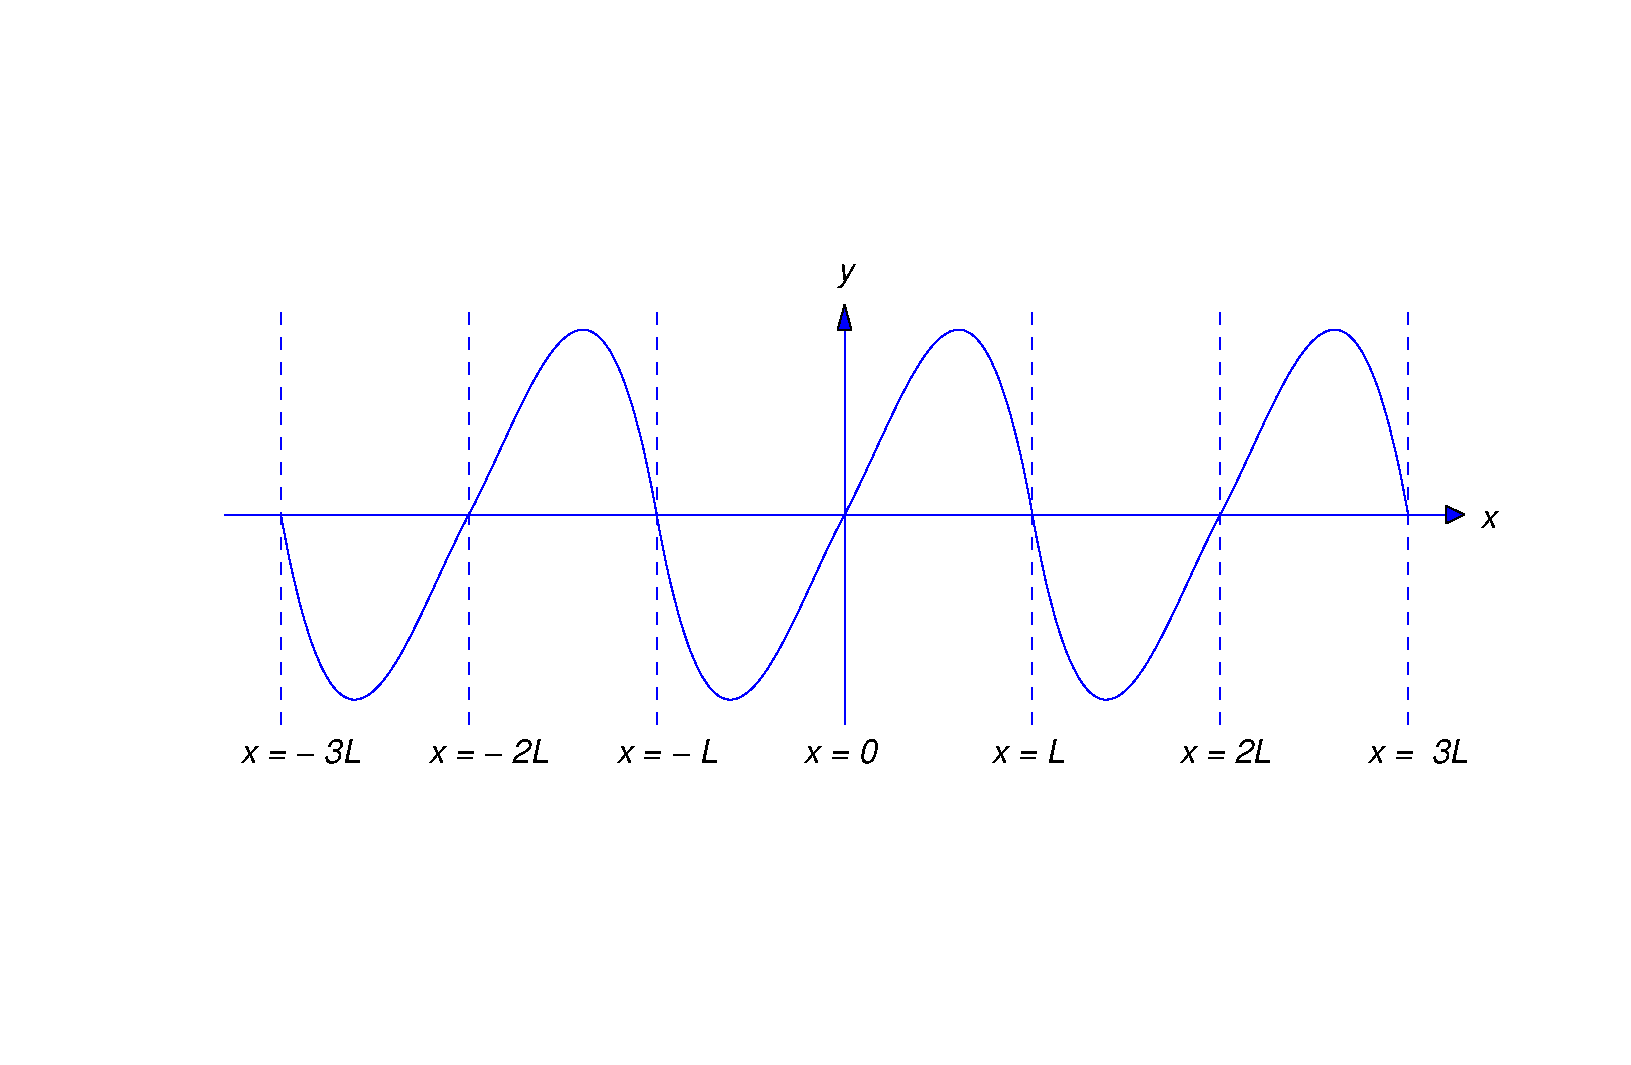
\includegraphics[bb=-78 148 689 643,width=5.67in,height=3.66in,keepaspectratio]{fig120204}}
\caption{ The odd extension of a function that
 satisfies \eqref{eq:12.2.13}}
  \label{figure:12.2.4}
\end{minipage}
\end{figure}

\part{b}
From Figure~\ref{figure:12.2.5},
$$
q'_-(2kL)=-h'_+(0)\mbox{\quad and \quad}  q'_+(2kL)=h'_+(0),
$$
so $q$ is differentiable at $x=2kL$ if and only if $h'_+(0)=0$.
Also,
$$
q'_-((2k-1)L)=h'_-(L) \mbox{\quad and \quad} q'_+((2k-1)L)=-h'_-(L),
$$
so $q$ is differentiable at $x=(2k-1)L$ if and only if $h'_-(L)=0$.
Therefore
 $q$  is differentiable on $(-\infty,\infty)$
if and only if $h'_+(0)=h'_-(L)=0$, as in Figure~\ref{figure:12.2.6}.
This completes the proof.

\begin{figure}[H]
\color{blue}
  \begin{minipage}[b]{0.5\linewidth}
    \centering
   \scalebox{.55}{
  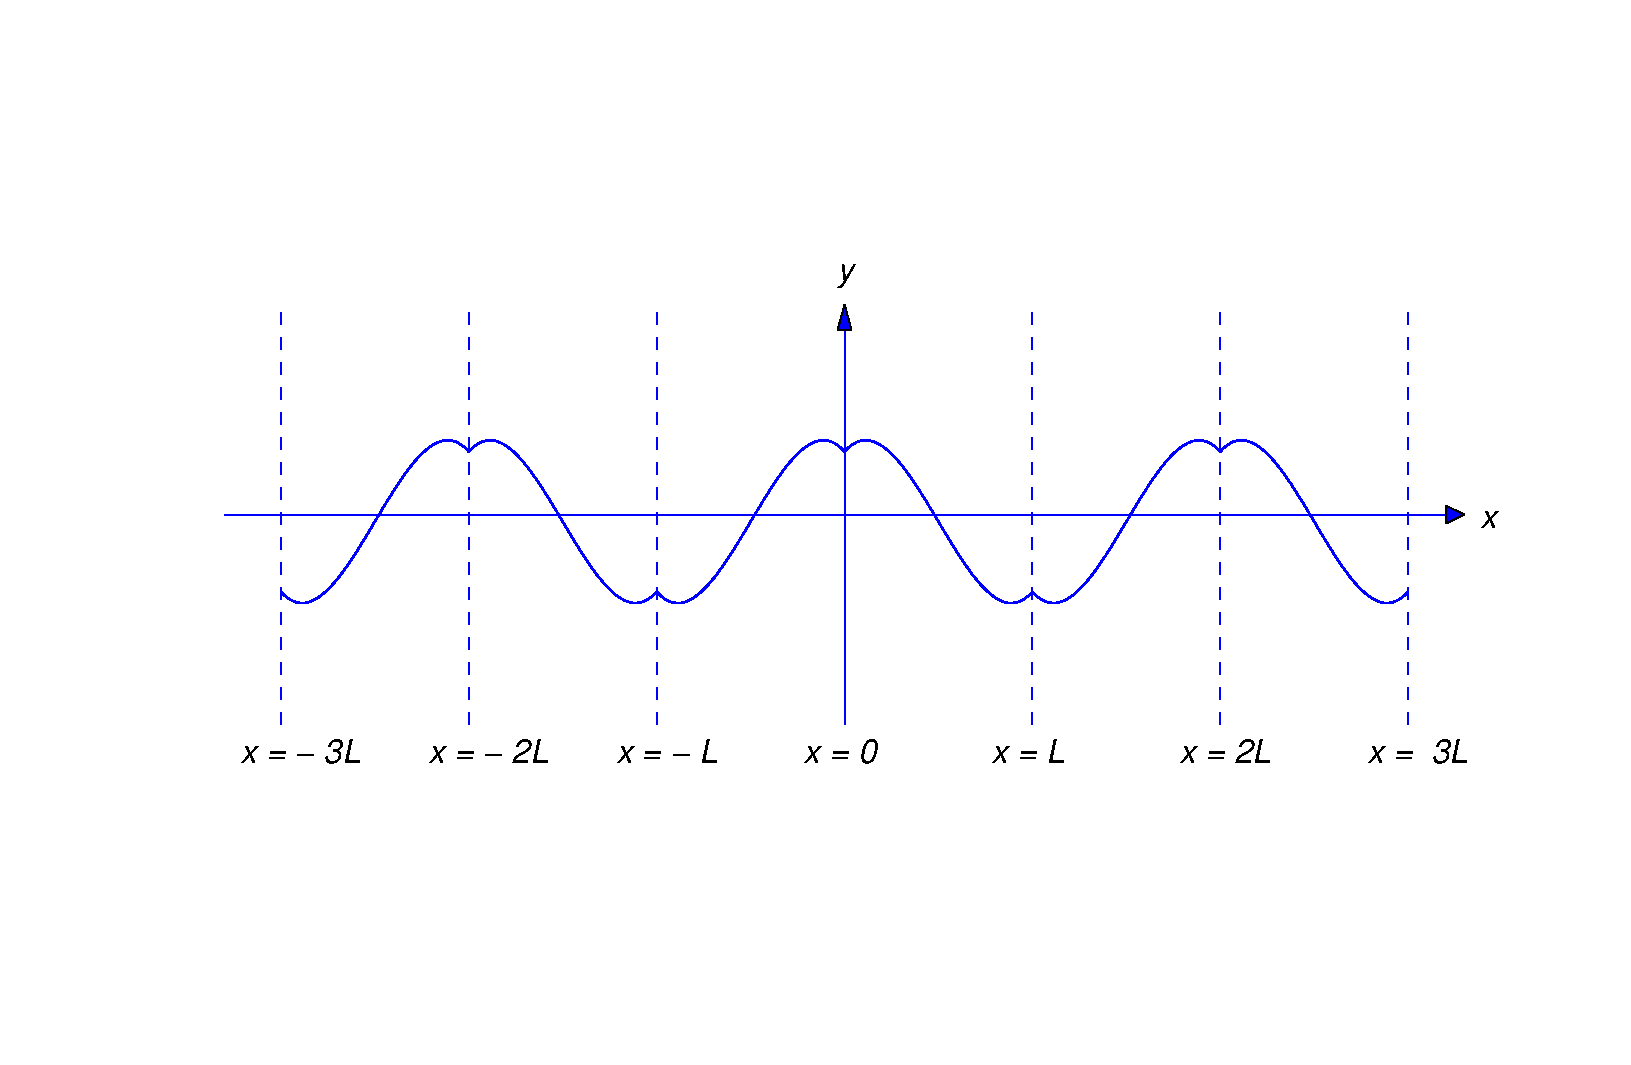
\includegraphics[bb=-78 148 689 643,width=5.67in,height=3.66in,keepaspectratio]{fig120205}}
\caption{ The even extension of a function that doesn't
 satisfy \eqref{eq:12.2.14}}
  \label{figure:12.2.5}
\end{minipage}
  \begin{minipage}[b]{0.5\linewidth}
    \centering
   \scalebox{.55}{
  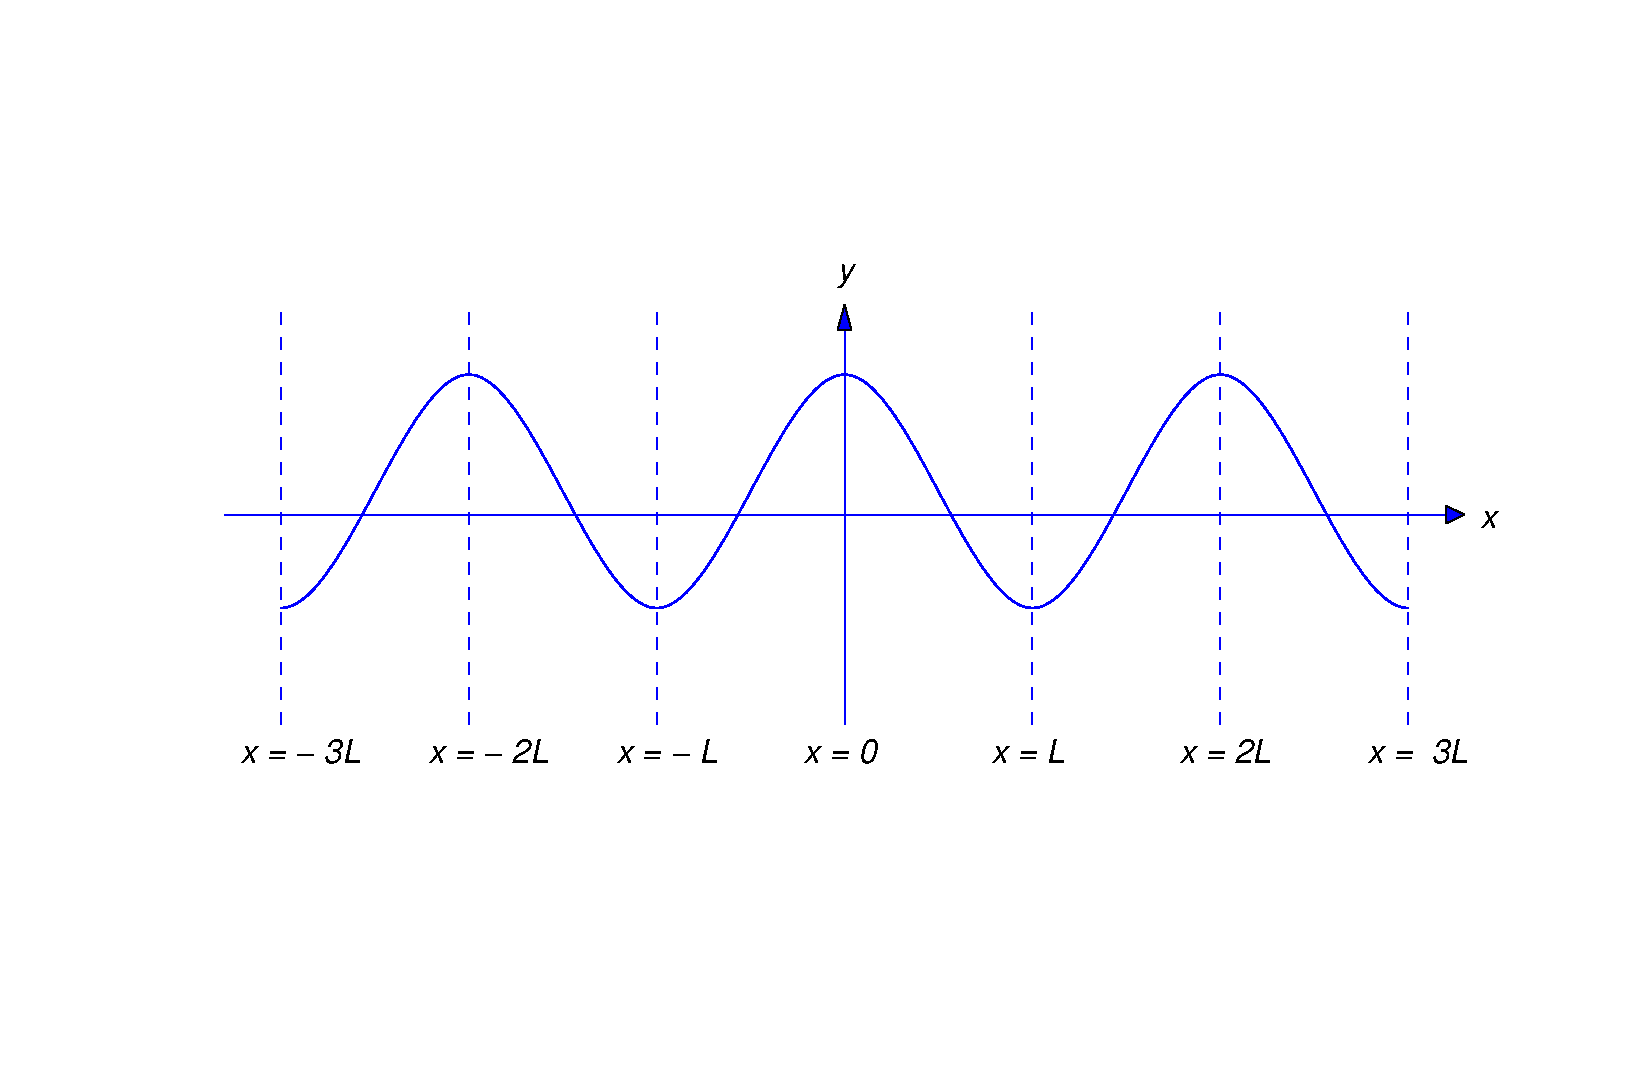
\includegraphics[bb=-78 148 689 643,width=5.67in,height=3.66in,keepaspectratio]{fig120206}}
\caption{ The even extension of a function that
 satisfies \eqref{eq:12.2.14}}
  \label{figure:12.2.6}
\end{minipage}
\end{figure}

\begin{theorem}\color{blue} \label{thmtype:12.2.4}
The formal solution of \eqref{eq:12.2.1}
is an actual solution if $g$ is differentiable on $[0,L]$
and
\begin{equation} \label{eq:12.2.15}
g(0)=g(L)=0,
\end{equation}
while $f$ is twice differentiable on $[0,L]$ and
\begin{equation} \label{eq:12.2.16}
f(0)=f(L)=0
\end{equation}
and
\begin{equation} \label{eq:12.2.17}
f''_+(0)=f''_-(L)=0.
\end{equation}
\end{theorem}

\proof
We first show that $S_g$ is differentiable and $S_f$
is twice differentiable on $(-\infty,\infty)$. We'll then
differentiate  \eqref{eq:12.2.9} twice with respect to $x$ and $t$
and verify that  \eqref{eq:12.2.9}  is an actual solution of \eqref{eq:12.2.1}.

Since  $f$ and $g$ are continuous on $(0,L)$,
 Theorem~\ref{thmtype:11.3.2} implies that
$S_f(x)=f(x)$ and $S_g(x)=g(x)$ on $[0,L]$. Therefore $S_f$
and $S_g$ are the odd periodic extensions  of $f$ and $g$.
 Since $f$ and $g$ are differentiable on $[0,L]$,
\eqref{eq:12.2.15},
\eqref{eq:12.2.16}, and  Theorem~\ref{thmtype:12.2.3}\part{a} imply that
$S_f$ and $S_g$ are differentiable on $(-\infty,\infty)$.

Since $S_f'(x)=f'(x)$ on $[0,L]$ (one-sided derivatives at the
endpoints), and
$S_f'$ is even
(the derivative of an odd function is even),
$S_f'$ is the even periodic extension of $f'$. By assumption, $f'$ is
differentiable on $[0,L]$. Because of \eqref{eq:12.2.17},
Theorem~\ref{thmtype:12.2.3}\part{b} with $h=f'$ and $q=S_f'$ implies that
$S_f''$ exists on $(-\infty,\infty)$.

Now we can differentiate \eqref{eq:12.2.9} twice with respect to $x$
and $t$:
$$
u_x(x,t)={1\over2}[S_f'(x+at)+S_f'(x-at)]+
{1\over2a}[S_g(x+at)-S_g(x-at)],
$$
\begin{equation} \label{eq:12.2.18}
u_{xx}(x,t)={1\over2}[S_f''(x+at)+S_f''(x-at)]+
{1\over2a}[S_g'(x+at)-S_g'(x-at)],
\end{equation}
\begin{equation} \label{eq:12.2.19}
u_t(x,t)={a\over2}[S_f'(x+at)-S_f'(x-at)]+
{1\over2}[S_g(x+at)+S_g(x-at)],
\end{equation}
and
\begin{equation} \label{eq:12.2.20}
u_{tt}(x,t)={a^2\over2}[S_f''(x+at)-S_f''(x-at)]+
{a\over2}[S_g'(x+at)-S_g'(x-at)].
\end{equation}
Comparing \eqref{eq:12.2.18}  and \eqref{eq:12.2.20} shows that
$u_{tt}(x,t)=a^2u_{xx}(x,t)$ for all $(x,t)$.

From \eqref{eq:12.2.8},  $u(0,t)=u(L,t)=0$
for all $t$. From \eqref{eq:12.2.9},
$u(x,0)=S_f(x)$ for all $x$, and therefore, in particular,
$$
u(x,0)=f(x),\quad 0\le x< L.
$$
 From \eqref{eq:12.2.19},
$u_t(x,0)=S_g(x)$ for all $x$, and therefore, in particular,
$$
u_t(x,0)=g(x),\quad 0\le x< L.
$$
Therefore $u$ is an actual solution of \eqref{eq:12.2.1}.
This completes the proof.

Eqn~\eqref{eq:12.2.9} is called
\href{https://mathshistory.st-andrews.ac.uk/Biographies/DAlembert/}
{\color{blue}\it d'Alembert's
 solution\/} of \eqref{eq:12.2.1}. Although
d'Alembert's solution   was useful
for proving Theorem~\ref{thmtype:12.2.4} and is very useful in a slightly
different context (Exercises~\ref{exer:12.2.63}-\ref{exer:12.2.68}),
\eqref{eq:12.2.8} is preferable for computational purposes.

\begin{example}\label{example:12.2.1} \rm
Solve \eqref{eq:12.2.1} with
$$
f(x)=x(x^3-2Lx^2+L^2)
\mbox{\quad and \quad}
g(x)=x(L-x).
$$
\end{example}

\solution
We leave it to you to verify that $f$ and $g$ satisfy the assumptions
of Theorem~\ref{thmtype:12.2.4}.

From Exercise~11.3.~\hspace*{-3pt}\ref{exer:11.3.39},
$$
S_f(x)={96L^4\over\pi^5}\sum_{n=1}^\infty{1\over(2n-1)^5}\sin{(2n-1)\pi
x\over L}.
$$
From Exercise~11.3.~\hspace*{-3pt}\ref{exer:11.3.36},
$$
S_g(x)={8L^2\over\pi^3}\sum_{n=1}^\infty{1\over(2n-1)^3}\sin{(2n-1)\pi
x\over L}.
$$
From \eqref{eq:12.2.8},
$$
\begin{array}{rcl}
u(x,t)&=&
\dst{96L^4\over\pi^5}\sum_{n=1}^\infty{1\over(2n-1)^5}
\cos{(2n-1)\pi a t\over L}\sin{(2n-1)\pi x\over L}\\&&+
\dst{8L^3\over a\pi^4}\sum_{n=1}^\infty{1\over(2n-1)^4}
\sin{(2n-1)\pi a t\over L}\sin{(2n-1)\pi x\over L}.
\end{array}
$$

Theorem~\ref{thmtype:12.1.2}  implies that $u_{xx}$
and $u_{tt}$    can be obtained by term
by term differentiation, for all
$(x,t)$, so $u_{tt}=a^2u_{xx}$ for all
$(x,t)$ (Exercise~\ref{exer:12.2.62}). Moreover,
Theorem~\ref{thmtype:11.3.2}
implies that $S_f(x)=f(x)$ and $S_g(x)=g(x)$ if $0\le x\le L$. Therefore
$u(x,0)=f(x)$ and $u_t(x,0)=g(x)$ if $0\le x\le L$.
Hence, $u$ is an actual solution of the initial-boundary
value problem.

\medskip

\color{blue}
\remark
{In solving a specific initial-boundary value problem \eqref{eq:12.2.1},
it's convenient to solve the problem with $g\equiv0$, then with
$f\equiv0$, and add the solutions to obtain the solution of the given
problem. Because of this, either $f\equiv0$ or $g\equiv0$ in all
the specific initial-boundary value problems in the exercises.}
\color{black}

\boxit{The Plucked String}

\noindent
If $f$ and $g$ don't satisfy the assumptions of
Theorem~\ref{thmtype:12.2.4}, then \eqref{eq:12.2.8} isn't  an actual
solution of \eqref{eq:12.2.1}   in fact, it can be shown that \eqref{eq:12.2.1}
doesn't have an
actual solution in this case. Nevertheless, $u$ is defined for all
$(x,t)$, and we can see from \eqref{eq:12.2.18} and \eqref{eq:12.2.20} that
$u_{tt}(x,t)=a^2u_{xx}(x,t)$ for all $(x,t)$ such that
$S_f''(x\pm at)$  and $S_g'(x\pm at)$ exist.  Moreover, $u$
may still provide a useful approximation to the vibration of the
string;    a laboratory experiment can confirm or deny this.

We'll now consider the initial-boundary value problem
 \eqref{eq:12.2.1}  with
\begin{equation} \label{eq:12.2.21}
f(x)=
\left\{\begin{array}{cl}
x,&0\le x\le{L\over2},\\L-x,&{L\over2}\le x\le L
\end{array}\right.
\end{equation}
and $g\equiv0$.
Since $f$ isn't  differentiable at $x=L/2$, it doesn't satisfy
the assumptions of Theorem~\ref{thmtype:12.2.4}, so the formal solution
of \eqref{eq:12.2.1} can't be an actual solution.
Nevertheless,
it's instructive to investigate the properties of the formal
solution.

The graph of $f$ is shown in Figure~\ref{figure:12.2.7}. Intuitively, we
are plucking the string by half its length at the middle. You're right
if you think this is an extraordinarily large displacement;
however, we could remove this objection by multiplying the function in
Figure~\ref{figure:12.2.7} by a small constant. Since this would just
multiply the formal solution by the same constant, we'll leave $f$ as
we've defined it. Similar comments apply to the exercises.

\begin{figure}[tbp]
  \centering\color{blue}
  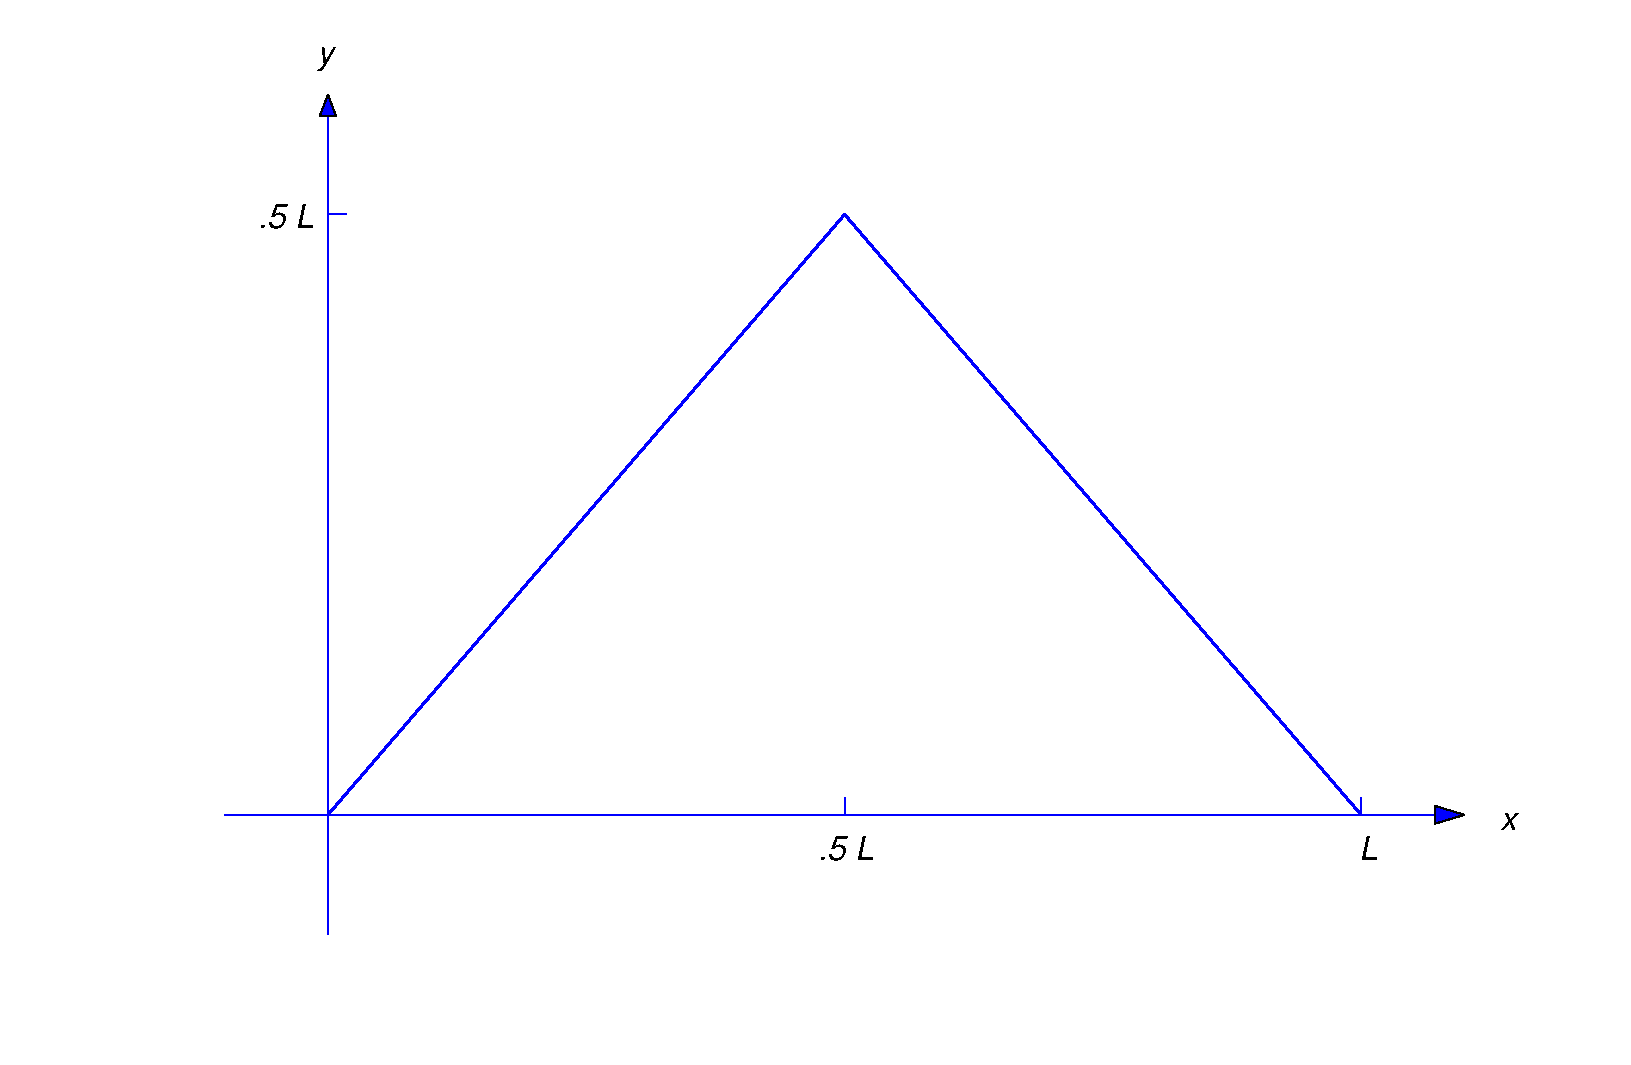
\includegraphics[bb=-78 148 689 643,width=5.67in,height=3.66in,keepaspectratio]{fig120207}
\caption{Graph of \eqref{eq:12.2.21}}
  \label{figure:12.2.7}
\end{figure}

From Exercise~11.3.~\hspace*{-3pt}\ref{exer:11.3.15}, the Fourier sine
series
of
$f$ on $[0,L]$ is
$$
S_f(x)=\dst{4L\over\pi^2}\sum_{n=1}^\infty{(-1)^{n+1}\over(2n-1)^2}
\sin{(2n-1)\pi x\over L},
$$
which converges to $f$ for all $x$ in $[0,L]$, by
Theorem~\ref{thmtype:11.3.2}. Therefore
\begin{equation} \label{eq:12.2.22}
u(x,t)=\dst{4L\over\pi^2}\sum_{n=1}^\infty{(-1)^{n+1}\over(2n-1)^2}
\cos{(2n-1)\pi at\over L}\sin{(2n-1)\pi x\over L}.
\end{equation}
This series converges absolutely for all $(x,t)$ by the comparison
test, since the series
$$
\sum_{n=1}^\infty{1\over(2n-1)^2}
$$
 converges. Moreover, \eqref{eq:12.2.22} satisfies the boundary
conditions
$$
u(0,t)=u(L,t)=0,\quad t>0,
$$
and the initial condition
$$
u(x,0)=f(x),\quad  0\le x\le L.
$$
However, we can't justify differentiating \eqref{eq:12.2.22} term by
term even once, and formally differentiating  it twice
term by term produces a series that diverges for all $(x,t)$.
(Verify.). Therefore
 we use
 d'Alembert's form
\begin{equation} \label{eq:12.2.23}
u(x,t)={1\over2}[S_f(x+at)+S_f(x-at)]
\end{equation}
for $u$ to study its derivatives.
Figure~\ref{figure:12.2.8} shows the graph of $S_f$, which is  the
odd periodic extension of $f$. You can see  from the graph
that $S_f$ is differentiable at  $x$ (and $S_f'(x)=\pm1$) if
and only if
$x$ isn't  an odd multiple of
$L/2$.

\begin{figure}[H]
\color{blue}
  \begin{minipage}[b]{0.5\linewidth}
    \centering
   \scalebox{.65}{
  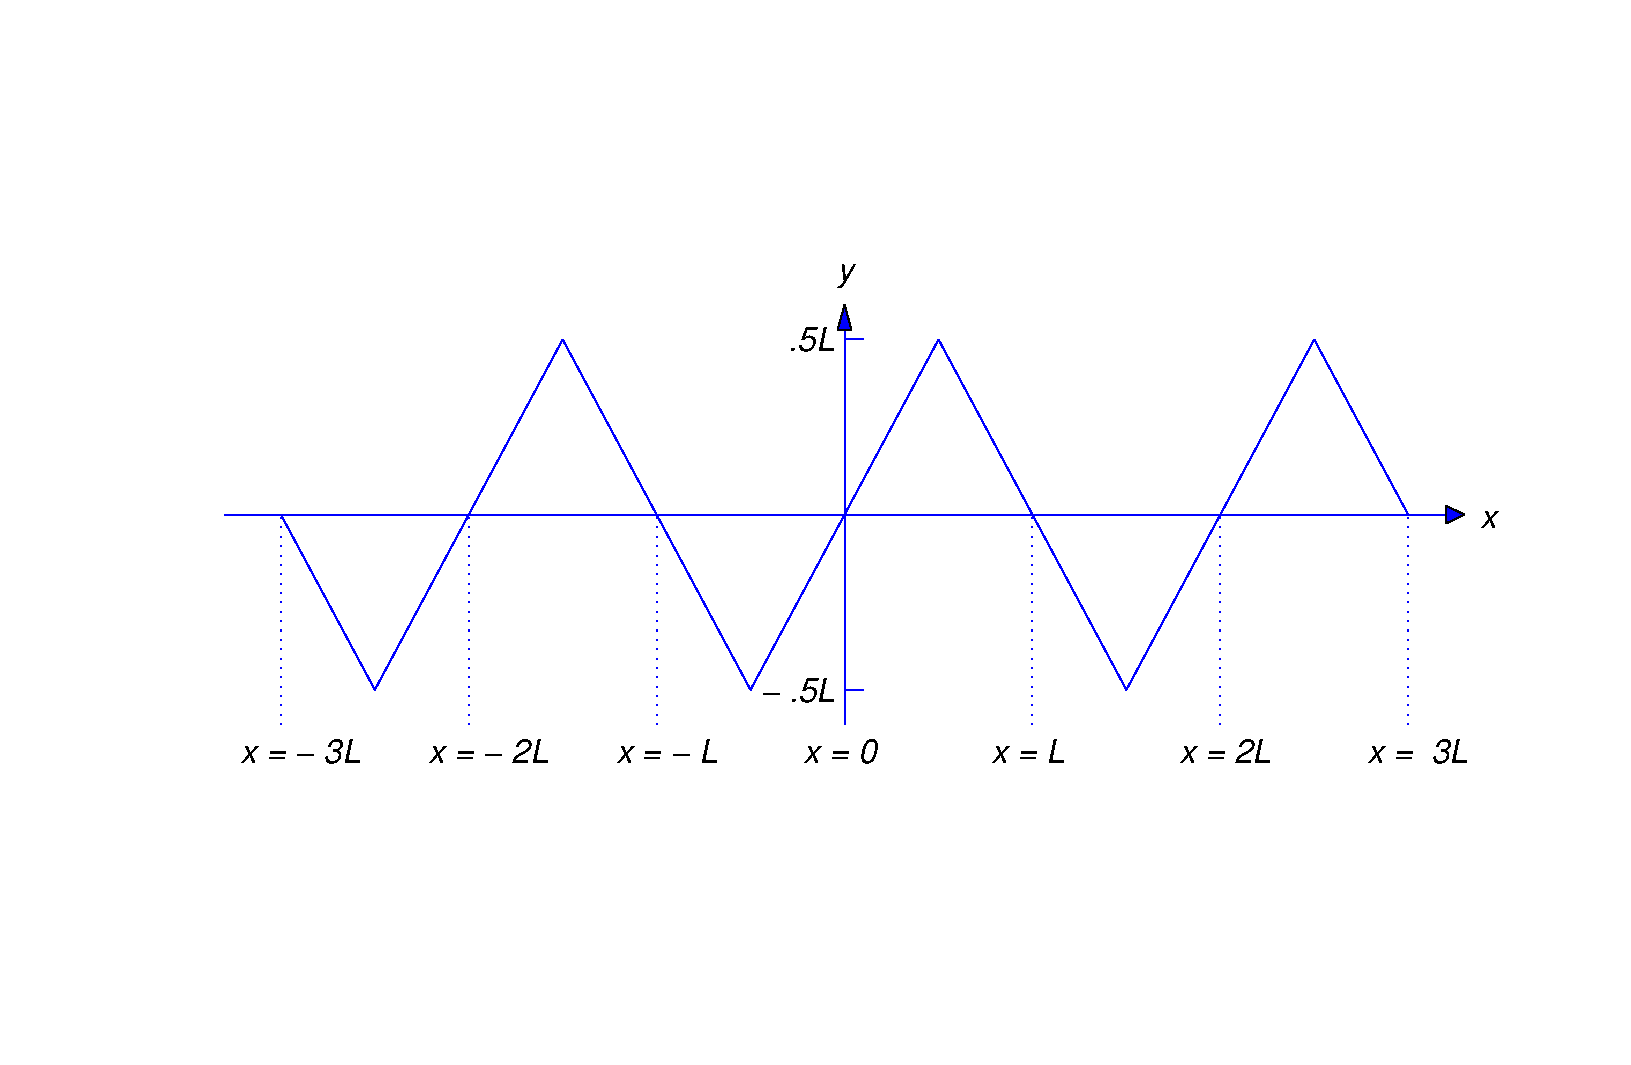
\includegraphics[bb=-78 148 689 643,width=5.67in,height=3.66in,keepaspectratio]{fig120208}}
\caption{ The odd periodic extension of
\eqref{eq:12.2.21}}
  \label{figure:12.2.8}
\end{minipage}
  \begin{minipage}[b]{0.5\linewidth}
    \centering
   \scalebox{.65}{
  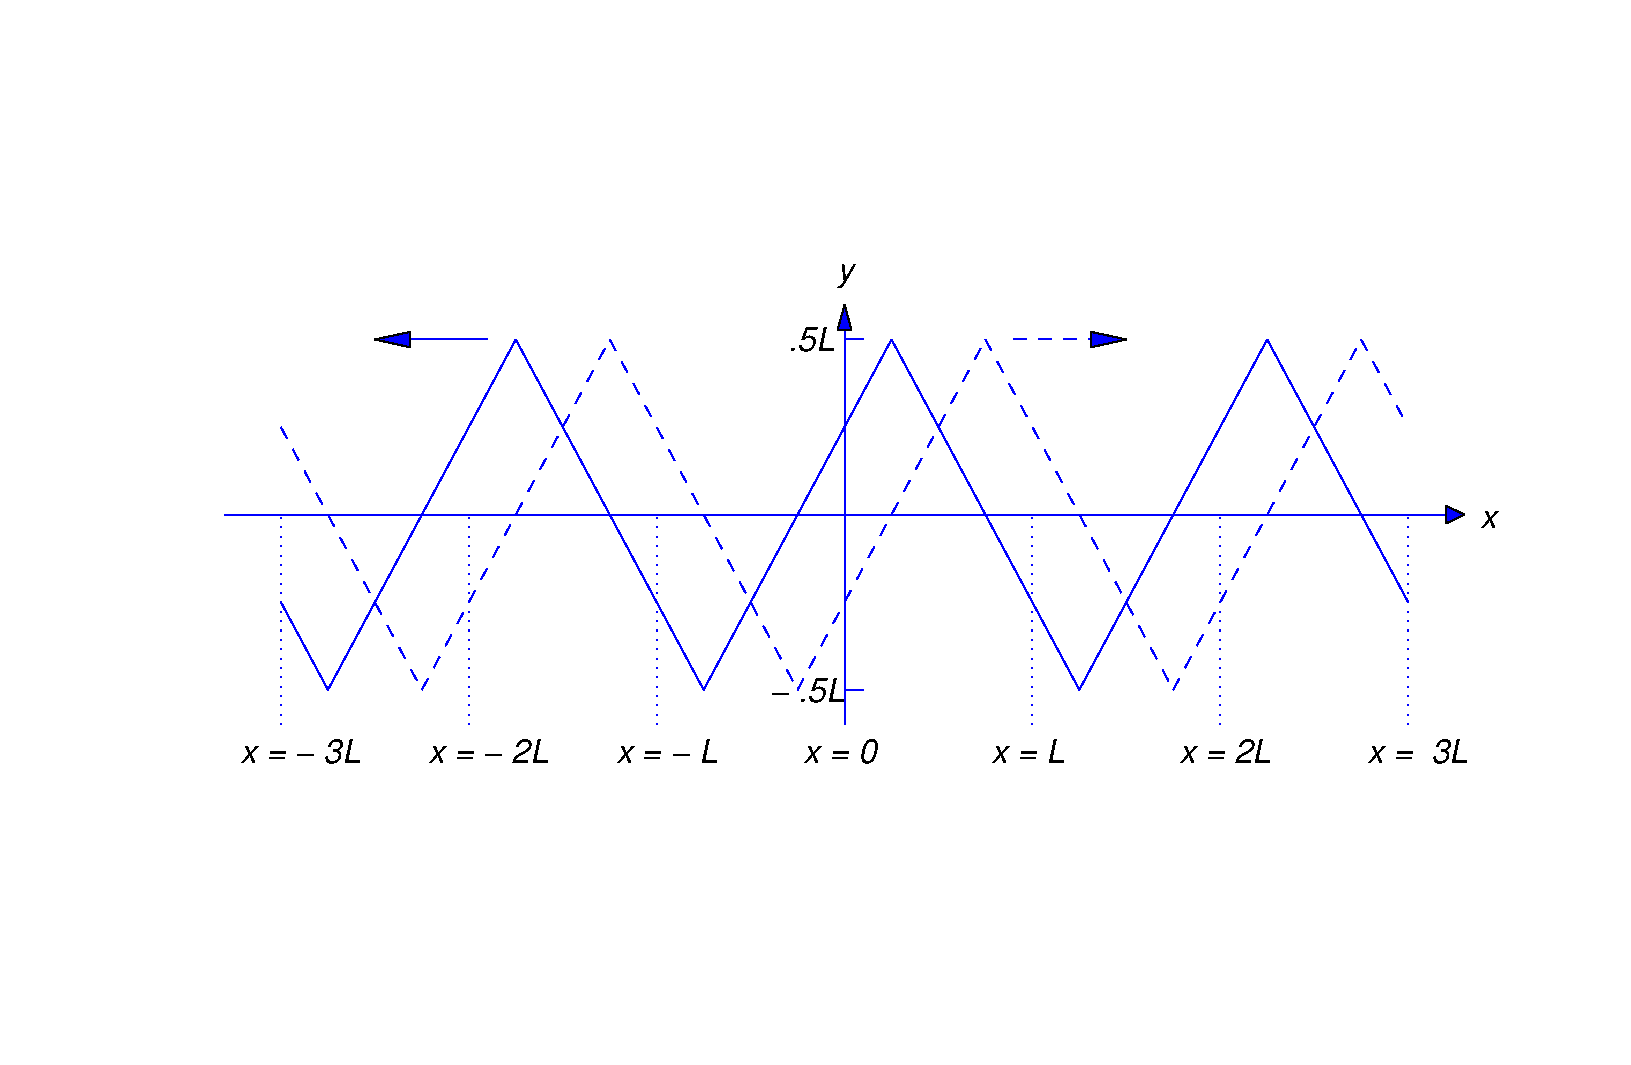
\includegraphics[bb=-78 148 689 643,width=5.67in,height=3.66in,keepaspectratio]{fig120209}}
\caption{ Graphs of $y=S_f(x-at)$ (dashed) and $y=S_f(x-at)$ (solid),
with $f$ as in \eqref{eq:12.2.21}}
  \label{figure:12.2.9}
\end{minipage}
\end{figure}

In Figure~\ref{figure:12.2.9} the
dashed and solid curves  are the graphs of $y=S_f(x-at)$ and
$y=S_f(x+at)$ respectively, for a fixed value of $t$.
As $t$ increases the dashed curve moves to the right and the solid
curve moves to the left. For this reason, we say that the functions
$u_1(x,t)=S_f(x+at)$ and $u_2(x,t)=S_f(x-at)$ are {\color{blue}\it traveling
waves\/}.
Note that $u_1$ satisfies the wave equation at $(x,t)$
if $x+at$ isn't  an odd multiple of $L/2$ and
 $u_2$ satisfies the wave equation at  $(x,t)$ if
$x-at$ isn't  an odd  multiple of $L/2$. Therefore \eqref{eq:12.2.23}
(or, equivalently, \eqref{eq:12.2.22})  satisfies
$u_{tt}(x,t)=a^2u_{xx}(x,t)=0$ for all $(x,t)$ such that neither
$x-at$ nor $x+at$ is an odd multiple of $L/2$.

We conclude by finding an  explicit formula for $u(x,t)$
 under the assumption that
\begin{equation} \label{eq:12.2.24}
0\le x\le L\mbox{\quad and \quad}0\le t\le L/2a.
\end{equation}
To see how this formula can be used to compute $u(x,t)$ for
$0\le x\le L$ and arbitrary
$t$, we refer you to Exercise~\ref{exer:12.2.16}.

From Figure~\ref{figure:12.2.10},
$$
S_f(x-at)=
\left\{\begin{array}{cl}
x-at,&0\le x\le {L\over2}+at,\\[2\jot]
L-x+at,&{L\over2}+at\le x\le L
\end{array}\right.
$$
and
$$
S_f(x+at)=
\left\{\begin{array}{cl}
x+at,&0\le x\le {L\over2}-at,\\[2\jot]
L-x-at,&{L\over2}-at\le x\le L
\end{array}\right.
$$
if $(x,t)$ satisfies \eqref{eq:12.2.24}.

Therefore, from \eqref{eq:12.2.23},
$$
u(x,t)=
\left\{\begin{array}{cl}
x,&0\le x\le{L\over2}-at,\\[2\jot]
{L\over2}-at,&{L\over2}-at\le x\le{L\over2}+at,\\[2\jot]
L-x,&{L\over2}-at\le x\le L
\end{array}\right.
$$
if $(x,t)$ satisfies \eqref{eq:12.2.24}. Figure~\ref{figure:12.2.11}
is the graph of this function on $[0,L]$ for a fixed $t$ in
$(0,L/2a)$.

\begin{figure}[H]
\color{blue}
  \begin{minipage}[b]{0.5\linewidth}
    \centering
   \scalebox{.65}{
  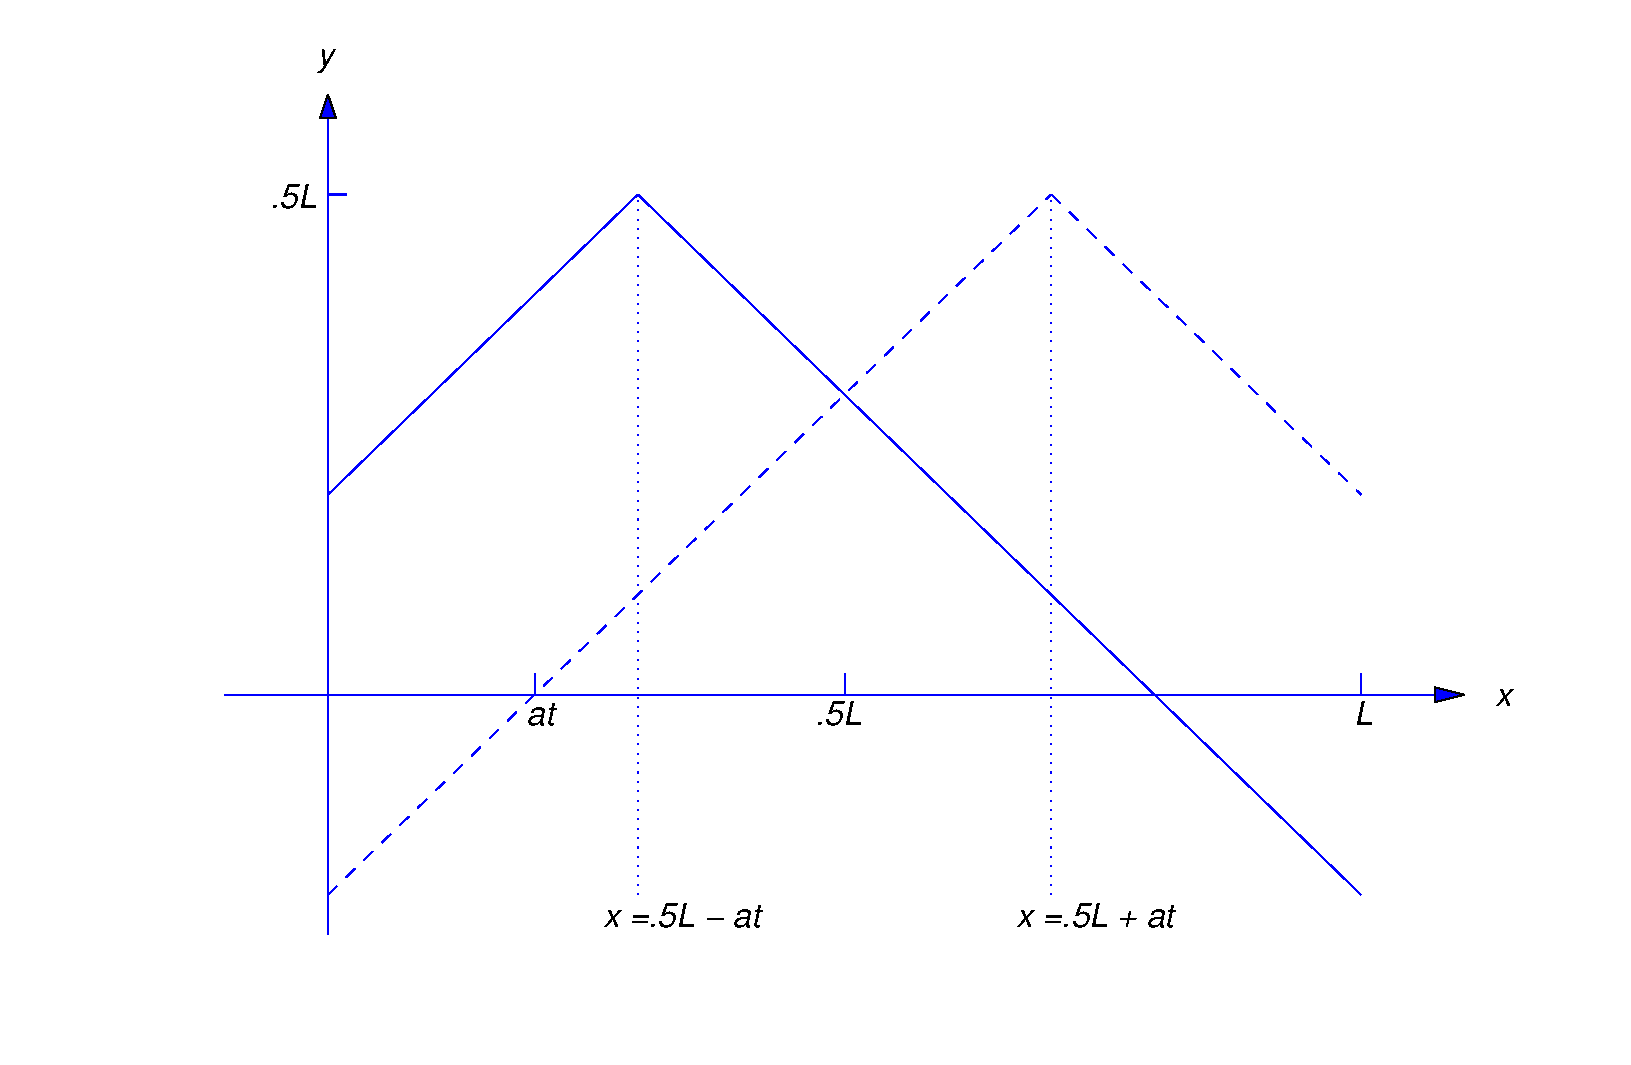
\includegraphics[bb=-78 148 689 643,width=5.67in,height=3.66in,keepaspectratio]{fig120210}}
\caption{ The part of the graph from Figure~\ref{figure:12.2.9} on $[0,L]$}
  \label{figure:12.2.10}
\end{minipage}
  \begin{minipage}[b]{0.5\linewidth}
    \centering
   \scalebox{.65}{
  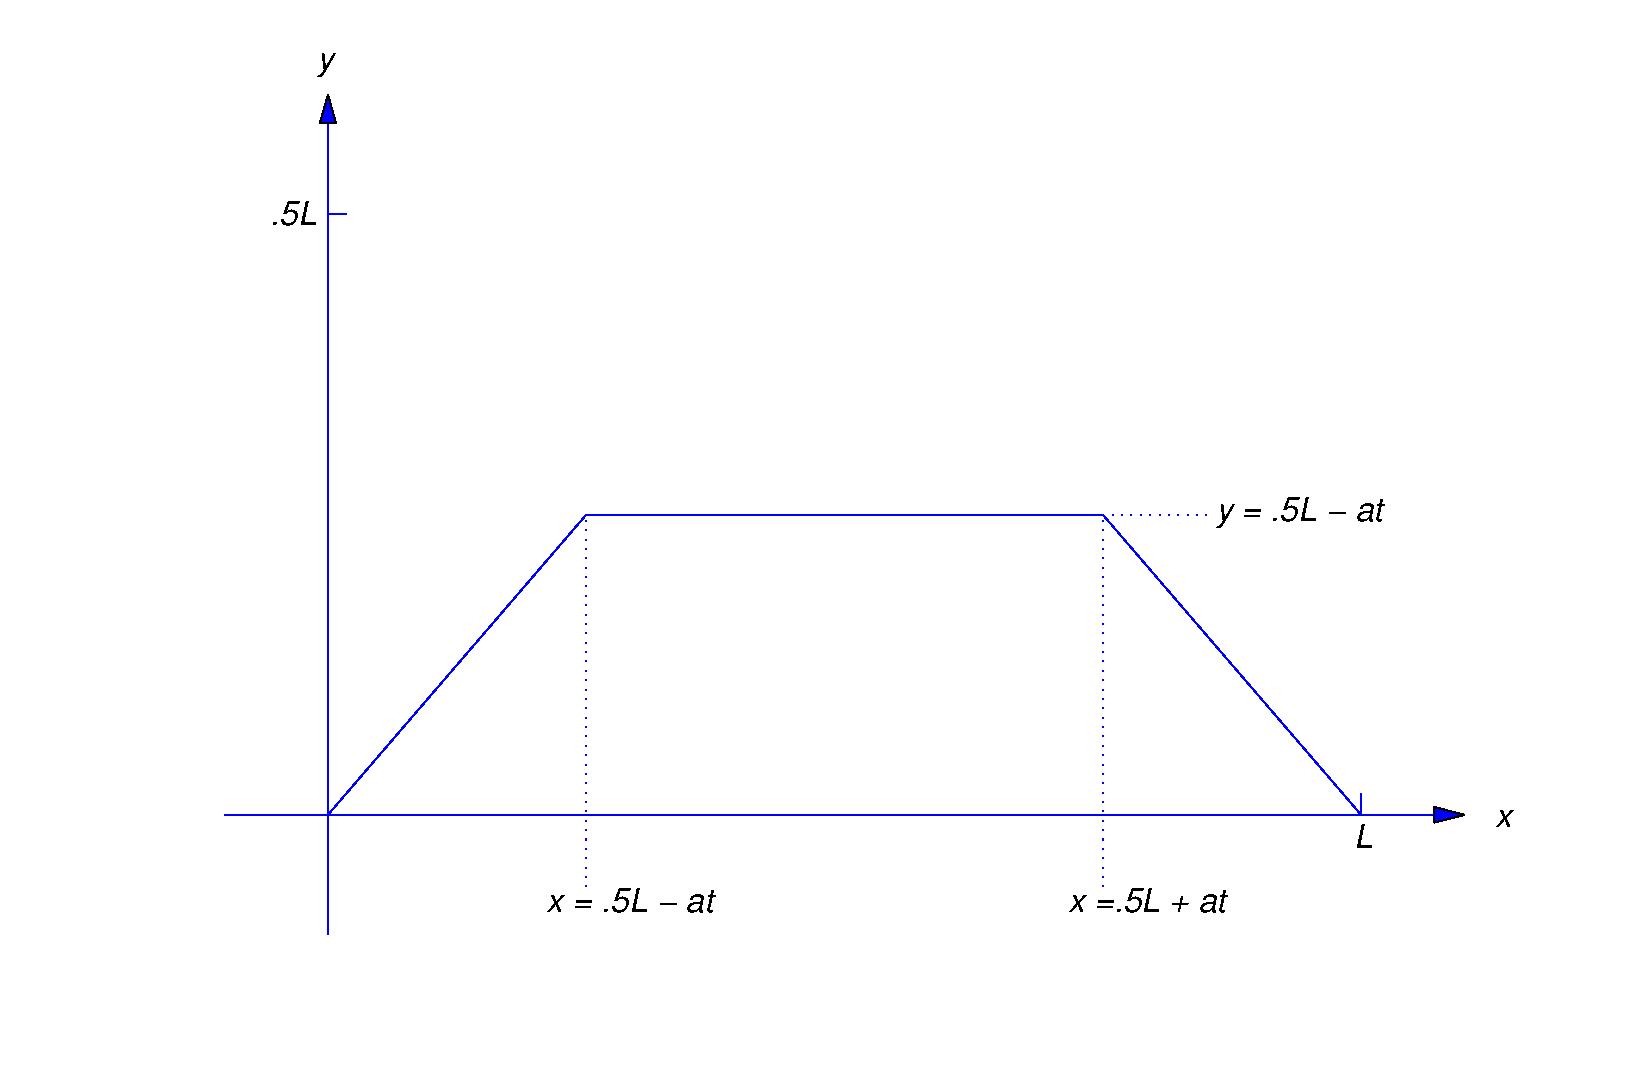
\includegraphics[bb=-78 148 689 643,width=5.67in,height=3.66in,keepaspectratio]{fig120211}}
\caption{ The graph of \eqref{eq:12.2.23} on $[0,L]$ for a fixed $t$ in
$(0,L/2a)$}
  \label{figure:12.2.11}
\end{minipage}
\end{figure}

\technology
\medskip

Although the formal solution
$$
u(x,t)=\sum_{n=1}^\infty\left(\alpha_n\cos{n\pi at\over
L}+{\beta_nL\over n\pi a}\sin{n\pi at\over L}\right)
\sin{n\pi x\over L}
$$
of \eqref{eq:12.2.1} is defined for all $(x,t)$, we're mainly interested
in its behavior for $0\le x\le L$ and $t\ge0$. In fact, it's
sufficient to consider only values of $t$ in the interval $0\le
t<2L/a$, since
$$
u(x,t+2kL/a)=u(x,t)
$$
for all $(x,t)$  if $k$ is an integer. (Verify.)

You can create an animation of the motion of the string
by performing the following numerical experiment.

Let $m$  and $k$ be positive integers. Let
$$
t_j={2Lj\over ka},\quad j=0,1,\dots k;
$$
thus, $t_0$, $t_1$, \dots $t_k$ are equally spaced points in $[0,2L/a]$.
For each $j=0$, $1$ ,$2$, \dots $k$, graph the partial sum
$$
u_m(x,t_j)=\sum_{n=1}^m\left(\alpha_n\cos{n\pi at_j\over
L}+{\beta_nL\over n\pi a}\sin{n\pi at_j\over L}\right)
\sin{n\pi x\over L}
$$
on $[0,L]$ as a function of $x$.  Write your program so that
each graph remains displayed on the monitor for a short time,
and is then deleted and replaced by the next. Repeat this
procedure for various values of $m$ and $k$.

We suggest that you perform experiments of this kind in the exercises
marked \Cex\hspace*{-3pt}, without other specific instructions. (These
exercises
were chosen arbitrarily;   the experiment is worthwhile in all the
exercises dealing with specific initial-boundary value problems.) In
some of the exercises the formal solutions have other forms, defined
in Exercises~\ref{exer:12.2.17}, \ref{exer:12.2.34}, and
\ref{exer:12.2.49};     however,
the idea of the experiment is the same.

\exercises
\noindent

\noindent
{\it In Exercises~\ref{exer:12.2.1}-\ref{exer:12.2.15} solve the
initial-boundary value problem.
In some of these exercises, Theorem~\ref{thmtype:11.3.5}\part{b}
or Exercise~$11.3$.~\hspace*{-3pt}\ref{exer:11.3.35} will
simplify the computation of the coefficients in the Fourier sine series.}

\begin{exerciselist}

\item\label{exer:12.2.1}
$u_{tt}=9u_{xx},\quad 0<x<1,\quad t>0$,\\
$u(0,t)=0,\quad u(1,t)=0,\quad t>0$,\\
$u(x,0)=0,\quad
 u_t(x,0)=
\left\{\begin{array}{cl}
x,&0\le x\le{1\over2},\\1-x,&{1\over2}\le x\le1
\end{array}\right.,\quad0\le x\le1$

\item\label{exer:12.2.2}
$u_{tt}=9u_{xx},\quad 0<x<1,\quad t>0$,\\
$u(0,t)=0,\quad u(1,t)=0,\quad t>0$,\\
$u(x,0)=x(1-x),\quad u_t(x,0)=0,\quad0\le x\le 1$

\item\label{exer:12.2.3}
$u_{tt}=7u_{xx},\quad 0<x<1,\quad t>0$,\\
$u(0,t)=0,\quad u(1,t)=0,\quad t>0$,\\
$u(x,0)=x^2(1-x),\quad u_t(x,0)=0,\quad0\le x\le1$

\item\label{exer:12.2.4}  \Cex
$u_{tt}=9u_{xx},\quad 0<x<1,\quad t>0$,\\
$u(0,t)=0,\quad u(1,t)=0,\quad t>0$,\\
$u(x,0)=0,\quad u_t(x,0)=x(1-x),\quad0\le x\le 1$

\item\label{exer:12.2.5}
$u_{tt}=7u_{xx},\quad 0<x<1,\quad t>0$,\\
$u(0,t)=0,\quad u(1,t)=0,\quad t>0$,\\
$u(x,0)=0\quad u_t(x,0)=x^2(1-x),\quad0\le x\le1$

\item\label{exer:12.2.6}
$u_{tt}=64u_{xx},\quad 0<x<3,\quad t>0$,\\
$u(0,t)=0,\quad u(3,t)=0,\quad t>0$,\\
$u(x,0)=x(x^2-9),\quad u_t(x,0)=0,\quad0\le x\le 3$

\item\label{exer:12.2.7}
$u_{tt}=4u_{xx},\quad 0<x<1,\quad t>0$,\\
$u(0,t)=0,\quad u(1,t)=0,\quad t>0$,\\
$u(x,0)=x(x^3-2x^2+1),\quad u_t(x,0)=0,\quad0\le x\le1$

\item\label{exer:12.2.8}  \Cex
$u_{tt}=64u_{xx},\quad 0<x<3,\quad t>0$,\\
  $u(0,t)=0,\quad u(3,t)=0,\quad t>0$,\\
$u(x,0)=0,\quad u_t(x,0)=x(x^2-9),\quad0\le x\le 3$

\item\label{exer:12.2.9}
$u_{tt}=4u_{xx},\quad 0<x<1,\quad t>0$,\\
$u(0,t)=0,\quad u(1,t)=0,\quad t>0$,\\
$u(x,0)=0,\quad u_t(x,0)=x(x^3-2x^2+1),\quad0\le x\le1$

\item\label{exer:12.2.10}
$u_{tt}=5u_{xx},\quad 0<x<\pi,\quad t>0$,\\
$u(0,t)=0,\quad u(\pi,t)=0,\quad t>0$,\\
$u(x,0)=x\sin x,\quad u_t(x,0)=0,\quad0\le x\le \pi$

\item\label{exer:12.2.11}
$u_{tt}=u_{xx},\quad 0<x<1,\quad t>0$,\\
$u(0,t)=0,\quad u(1,t)=0,\quad t>0$,\\
$u(x,0)=x(3x^4-5x^3+2),\quad u_t(x,0)=0,\quad0\le x\le1$

\item\label{exer:12.2.12}   \Cex
$u_{tt}=5u_{xx},\quad 0<x<\pi,\quad t>0$,\\
$u(0,t)=0,\quad u(\pi,t)=0,\quad t>0$,\\
$u(x,0)=0,\quad u_t(x,0)=x\sin x,\quad0\le x\le \pi$

\item\label{exer:12.2.13}
$u_{tt}=u_{xx},\quad 0<x<1,\quad t>0$,\\
$u(0,t)=0,\quad u(1,t)=0,\quad t>0$,\\
$u(x,0)=0,\quad u_t(x,0)=x(3x^4-5x^3+2),\quad0\le x\le1$

\item\label{exer:12.2.14}
$u_{tt}=9u_{xx},\quad 0<x<1,\quad t>0$,\\
$u(0,t)=0,\quad u(1,t)=0,\quad t>0$,\\
$u(x,0)=x(3x^4-10x^2+7),\quad u_t(x,0)=0,\quad0\le x\le1$

\item\label{exer:12.2.15}   \Cex
$u_{tt}=9u_{xx},\quad 0<x<1,\quad t>0$,\\
$u(0,t)=0,\quad u(1,t)=0,\quad t>0$,\\
$u(x,0)=0\quad u_t(x,0)=x(3x^4-10x^2+7),\quad0\le x\le1$

\item\label{exer:12.2.16}
We saw
that the displacement of the plucked string is,
on the one hand,
$$
u(x,t)=\dst{4L\over\pi^2}\sum_{n=1}^\infty{(-1)^{n+1}\over(2n-1)^2}
\cos{(2n-1)\pi at\over L}\sin{(2n-1)\pi x\over L},\; 0\le x\le
L,\; t\ge 0,
\eqno{\rm(A)}
$$
and, on the other hand,
$$
u(x,\tau)=
\left\{\begin{array}{cl}
x,&0\le x\le{L\over2}-a\tau,\\[2\jot]
{L\over2}-a\tau,&{L\over2}-a\tau\le x\le{L\over2}+a\tau,\\[2\jot]
L-x,&{L\over2}-a\tau\le x\le L.
\end{array}\right.
\eqno{\rm(B)}
$$
if $0\le \tau\le L/2a$.
The first objective  of this exercise is to show that (B) can be used
to compute $u(x,t)$ for  $0\le x\le L$ and all $t>0$.
\begin{alist}
\item % (a)
Show that if $t>0$,  there's a nonnegative integer
$m$ such that either
$$
\mbox{\bf(i)}\quad t={mL\over a}+\tau\mbox{\quad or \quad}
\mbox{\bf(ii)}\quad t={(m+1)L\over a}-\tau,
$$
where $0\le \tau\le L/2a$.
\item % (b)
Use (A) to show that $u(x,t)=(-1)^mu(x,\tau)$ if \part{i}
holds, while $u(x,t)=(-1)^{m+1}u(x,\tau)$ if \part{ii} holds.
\item % (c)
\Lex\;  Perform the following experiment for specific values
of $L$ and $a$ and various values of $m$ and $k$:
 Let
$$
t_j={Lj\over 2ka},\quad j=0,1,\dots k;
$$
thus, $t_0$, $t_1$, \dots, $t_k$ are equally spaced points in $[0,L/2a]$.
For each $j=0$, $1$ , $2$,\dots, $k$, graph the $m$th partial sum
of (A) and $u(x,t_j)$ computed from (B) on the same axis.
Create an animation, as described in the remarks on using
technology at the end of the section.
\end{alist}

\item\label{exer:12.2.17}
If a string vibrates with the end at $x=0$ free to move in a
frictionless
vertical track and the end at $x=L$ fixed, then the initial-boundary
value problem for its displacement takes the form
$$
\begin{array}{c}
u_{tt}=a^2u_{xx},\quad 0<x<L,\quad t>0,\\
 u_x(0,t)=0,\quad u(L,t)=0,\quad t>0,\\
u(x,0)=f(x),\quad u_t(x,0)=g(x),\quad 0\le x\le L.
\end{array}
\eqno{\rm(A)}
$$
Justify defining the formal solution of (A) to be
$$
u(x,t)=\sum_{n=1}^\infty
\left(\alpha_n\cos{(2n-1)\pi a
t\over2L}+{2L\beta_n\over(2n-1)\pi a}\sin{(2n-1)\pi
at\over2L}\right)
\cos{(2n-1)\pi
x\over2L},
$$
where
$$
C_{M\!f}(x)=\sum_{n=1}^\infty\alpha_n\cos{(2n-1)\pi x\over2L}
\mbox{\quad and \quad}
C_{M\!g}(x)=\sum_{n=1}^\infty\beta_n\cos{(2n-1)\pi x\over2L}
$$
are the mixed Fourier cosine series of $f$ and $g$
on $[0,L]$; that is,
$$
\alpha_n={2\over L}\int_0^Lf(x)\cos{(2n-1)\pi x\over2L}\,dx
\mbox{\quad and \quad}
\beta_n={2\over L}\int_0^Lg(x)\cos{(2n-1)\pi x\over2L}\,dx.
$$

\exercisetext{
In Exercises~\ref{exer:12.2.18}-\ref{exer:12.2.31}, use
Exercise~\ref{exer:12.2.17} to solve the initial-boundary
value problem.  In some of these exercises
Theorem~\ref{thmtype:11.3.5}\part{c}
or Exercise~$11.3$.~\hspace*{-3pt}\ref{exer:11.3.42}\part{b} will simplify
the
computation of the coefficients in the mixed Fourier cosine series.}

\item\label{exer:12.2.18}
$u_{tt}=9u_{xx},\quad 0<x<2,\quad t>0$,\\
$u_x(0,t)=0,\quad u(2,t)=0,\quad t>0$,\\
$u(x,0)=4-x^2,\quad u_t(x,0)=0,\quad0\le x\le2$

\item\label{exer:12.2.19}
$u_{tt}=4u_{xx},\quad 0<x<1,\quad t>0$,\\
$u_x(0,t)=0,\quad u(1,t)=0,\quad t>0$,\\
$u(x,0)=x^2(1-x),\quad u_t(x,0)=0,\quad0\le x\le 1$

\item\label{exer:12.2.20}
$u_{tt}=9u_{xx},\quad 0<x<2,\quad t>0$,\\
$u_x(0,t)=0,\quad u(2,t)=0,\quad t>0$,\\
$u(x,0)=0,\quad u_t(x,0)=4-x^2,\quad0\le x\le2$

\item\label{exer:12.2.21}
$u_{tt}=4u_{xx},\quad 0<x<1,\quad t>0$,\\
$u_x(0,t)=0,\quad u(1,t)=0,\quad t>0$,\\
$u(x,0)=0,\quad u_t(x,0)=x^2(1-x),\quad0\le x\le 1$

\item\label{exer:12.2.22}  \Cex
$u_{tt}=5u_{xx},\quad 0<x<1,\quad t>0$,\\
$u_x(0,t)=0,\quad u(1,t)=0,\quad t>0$,\\
$u(x,0)=2x^3+3x^2-5,\quad u_t(x,0)=0,\quad0\le x\le1$

\item\label{exer:12.2.23}
$u_{tt}=3u_{xx},\quad 0<x<\pi,\quad t>0$,\\
$u_x(0,t)=0,\quad u(\pi,t)=0,\quad t>0$,\\
$u(x,0)=\pi^3-x^3,\quad u_t(x,0)=0,\quad0\le x\le\pi$

\item\label{exer:12.2.24}
$u_{tt}=5u_{xx},\quad 0<x<1,\quad t>0$,\\
$u_x(0,t)=0,\quad u(1,t)=0,\quad t>0$,\\
$u(x,0)=0,\quad u_t(x,0)=2x^3+3x^2-5,\quad0\le x\le1$

\item\label{exer:12.2.25}   \Cex
$u_{tt}=3u_{xx},\quad 0<x<\pi,\quad t>0$,\\
$u_x(0,t)=0,\quad u(\pi,t)=0,\quad t>0$,\\
$u(x,0)=0,\quad u_t(x,0)=\pi^3-x^3,\quad0\le x\le\pi$

\item\label{exer:12.2.26}
$u_{tt}=9u_{xx},\quad 0<x<1,\quad t>0$,\\
$u_x(0,t)=0,\quad u(1,t)=0,\quad t>0$,\\
$u(x,0)=x^4-2x^3+1,\quad u_t(x,0)=0,\quad0\le x\le1$

\item\label{exer:12.2.27}
$u_{tt}=7u_{xx},\quad 0<x<1,\quad t>0$,\\
$u_x(0,t)=0,\quad u(1,t)=0,\quad t>0$,\\
$u(x,0)=4x^3+3x^2-7,\quad u_t(x,0)=0,\quad0\le x\le1$

\item\label{exer:12.2.28}
$u_{tt}=9u_{xx},\quad 0<x<1,\quad t>0$,\\
$u_x(0,t)=0,\quad u(1,t)=0,\quad t>0$,\\
$u(x,0)=0,\quad u_t(x,0)=x^4-2x^3+1,\quad0\le x\le1$

\item\label{exer:12.2.29}   \Cex
$u_{tt}=7u_{xx},\quad 0<x<1,\quad t>0$,\\
$u_x(0,t)=0,\quad u(1,t)=0,\quad t>0$,\\
$u(x,0)=0,\quad u_t(x,0)=4x^3+3x^2-7,\quad0\le x\le1$

\item\label{exer:12.2.30}
$u_{tt}=u_{xx},\quad 0<x<1,\quad t>0$,\\
$u_x(0,t)=0,\quad u(1,t)=0,\quad t>0$,\\
$u(x,0)=x^4-4x^3+6x^2-3,\quad u_t(x,0)=0,\quad0\le x\le1$

\item\label{exer:12.2.31}
$u_{tt}=u_{xx},\quad 0<x<1,\quad t>0$,\\
$u_x(0,t)=0,\quad u(1,t)=0,\quad t>0$,\\
$u(x,0)=0,\quad u_t(x,0)=x^4-4x^3+6x^2-3,\quad0\le x\le1$

\item\label{exer:12.2.32} Adapt the proof of Theorem~\ref{thmtype:12.2.2}
to find d'Alembert's solution of the initial-boundary value problem
in Exercise~\ref{exer:12.2.17}.

\item\label{exer:12.2.33}
Use the result of Exercise~\ref{exer:12.2.32} to show that the formal
solution of the initial-boundary value problem in
Exercise~\ref{exer:12.2.17}
is an actual solution if $g$ is differentiable and $f$ is twice
differentiable on $[0,L]$ and
$$
g'_+(0)=g(L)=f'_+(0)=f(L)=f''_-(L)=0.
$$
\hint{See Exercise~$11.3$.~\hspace*{-3pt}\ref{exer:11.3.57},
and apply Theorem~\ref{thmtype:12.2.3} with
$L$ replaced by $2L$.}

\item\label{exer:12.2.34}
Justify  defining the formal solution of the initial-boundary
value problem
$$
\begin{array}{c}
u_{tt}=a^2u_{xx},\quad 0<x<L,\quad t>0,\\
 u(0,t)=0,\quad u_x(L,t)=0,\quad t>0,\\
u(x,0)=f(x),\quad u_t(x,0)=g(x),\quad 0\le x\le L
\end{array}
$$
to be
$$
u(x,t)=\sum_{n=1}^\infty
\left(\alpha_n\cos{(2n-1)\pi a
t\over2L}+{2L\beta_n\over(2n-1)\pi a}\sin{(2n-1)\pi
at\over2L}\right)
\sin{(2n-1)\pi x\over2L},
$$
where
$$
S_{M\!f}(x)=\sum_{n=1}^\infty\alpha_n\sin{(2n-1)\pi x\over2L}
\mbox{\quad and \quad}
S_{M\!g}(x)=\sum_{n=1}^\infty\beta_n\sin{(2n-1)\pi x\over2L}
$$
are the mixed Fourier sine series of $f$ and $g$
on $[0,L]$; that is,
$$
\alpha_n={2\over L}\int_0^Lf(x)\sin{(2n-1)\pi x\over2L}\,dx
\mbox{\quad and \quad}
\beta_n={2\over L}\int_0^Lg(x)\sin{(2n-1)\pi x\over2L}\,dx.
$$

\exercisetext{
In Exercises~\ref{exer:12.2.35}-\ref{exer:12.2.46} use
Exercise~\ref{exer:12.2.34} to solve the initial-boundary
value problem.  In some of these exercises
Theorem~\ref{thmtype:11.3.5}\part{d}
or Exercise~$11.3$.~\hspace*{-3pt}\ref{exer:11.3.50}\part{b} will simplify
the
computation of the coefficients in the mixed Fourier sine series.}

\item\label{exer:12.2.35}
$u_{tt}=64u_{xx},\quad 0<x<\pi,\quad t>0$,\\
$u(0,t)=0,\quad u_x(\pi,t)=0,\quad t>0$,\\
$u(x,0)=x(2\pi-x),\quad u_t(x,0)=0,\quad0\le x\le \pi$

\item\label{exer:12.2.36}
$u_{tt}=9u_{xx},\quad 0<x<1,\quad t>0$,\\
$u(0,t)=0,\quad u_x(1,t)=0,\quad t>0$,\\
$u(x,0)=x^2(3-2x),\quad u_t(x,0)=0,\quad0\le x\le 1$

\item\label{exer:12.2.37}
$u_{tt}=64u_{xx},\quad 0<x<\pi,\quad t>0$,\\
$u(0,t)=0,\quad u_x(\pi,t)=0,\quad t>0$,\\
$u(x,0)=0,\quad u_t(x,0)=x(2\pi-x),\quad0\le x\le \pi$

\item\label{exer:12.2.38}   \Cex
$u_{tt}=9u_{xx},\quad 0<x<1,\quad t>0$,\\
$u(0,t)=0,\quad u_x(1,t)=0,\quad t>0$,\\
$u(x,0)=0,\quad u_t(x,0)=x^2(3-2x),\quad0\le x\le 1$

\item\label{exer:12.2.39}
$u_{tt}=9u_{xx},\quad 0<x<1,\quad t>0$,\\
$u(0,t)=0,\quad u_x(1,t)=0,\quad t>0$,\\
$u(x,0)=(x-1)^3+1,\quad u_t(x,0)=0,\quad0\le x\le 1$

\item\label{exer:12.2.40}
$u_{tt}=3u_{xx},\quad 0<x<\pi,\quad t>0$,\\
$u(0,t)=0,\quad u_x(\pi,t)=0,\quad t>0$,\\
$u(x,0)=x(x^2-3\pi^2),\quad u_t(x,0)=0,\quad0\le x\le\pi$

\item\label{exer:12.2.41}
$u_{tt}=9u_{xx},\quad 0<x<1,\quad t>0$,\\
$u(0,t)=0,\quad u_x(1,t)=0,\quad t>0$,\\
$u(x,0)=0,\quad u_t(x,0)=(x-1)^3+1,\quad0\le x\le 1$

\item\label{exer:12.2.42}
$u_{tt}=3u_{xx},\quad 0<x<\pi,\quad t>0$,\\
$u(0,t)=0,\quad u_x(\pi,t)=0,\quad t>0$,\\
$u(x,0)=0,\quad u_t(x,0)=x(x^2-3\pi^2),\quad0\le x\le\pi$

\item\label{exer:12.2.43}
$u_{tt}=5u_{xx},\quad 0<x<1,\quad t>0$,\\
$u(0,t)=0,\quad u_x(1,t)=0,\quad t>0$,\\
$u(x,0)=x^3(3x-4),\quad u_t(x,0)=0,\quad0\le x\le1$

\item\label{exer:12.2.44} \Cex
$u_{tt}=16u_{xx},\quad 0<x<1,\quad t>0$,\\
$u(0,t)=0,\quad u_x(1,t)=0,\quad t>0$,\\
$u(x,0)=x(x^3-2x^2+2),\quad u_t(x,0)=0,\quad0\le x\le1$

\item\label{exer:12.2.45}
$u_{tt}=5u_{xx},\quad 0<x<1,\quad t>0$,\\
$u(0,t)=0,\quad u_x(1,t)=0,\quad t>0$,\\
$u(x,0)=0,\quad u_t(x,0)=x^3(3x-4),\quad0\le x\le1$

\item\label{exer:12.2.46}  \Cex
$u_{tt}=16u_{xx},\quad 0<x<1,\quad t>0$,\\
$u(0,t)=0,\quad u_x(1,t)=0,\quad t>0$,\\
$u(x,0)=0,\quad u_t(x,0)=x(x^3-2x^2+2),\quad0\le x\le1$

\item\label{exer:12.2.47} Adapt the proof of Theorem~\ref{thmtype:12.2.2}
to find d'Alembert's solution of the initial-boundary value problem
in Exercise~\ref{exer:12.2.34}.

\item\label{exer:12.2.48}
Use the result of Exercise~\ref{exer:12.2.47} to show that the formal
solution of the initial-boundary value problem in
Exercise~\ref{exer:12.2.34}
is an actual solution if $g$ is differentiable and $f$ is twice
differentiable on $[0,L]$ and
$$
f(0)=f'_-(L)=g(0)=g_-'(L)=f''_+(0)=0.
$$
\hint{See Exercise~$11.3$.~\hspace*{-3pt}\ref{exer:11.3.58}
and apply Theorem~\ref{thmtype:12.2.3} with
$L$ replaced by $2L$.}

\item\label{exer:12.2.49}
Justify  defining the formal solution of the initial-boundary
value problem
$$
\begin{array}{c}
u_{tt}=a^2u_{xx},\quad 0<x<L,\quad t>0,\\
 u_x(0,t)=0,\quad u_x(L,t)=0,\quad t>0,\\
u(x,0)=f(x),\quad u_t(x,0)=g(x),\quad 0\le x\le L.
\end{array}
$$
to be
$$
u(x,t)=\alpha_0+\beta_0t+\sum_{n=1}^\infty
\left(\alpha_n\cos{n\pi at\over L}+{L\beta_n\over n\pi
a}\sin{n\pi at\over L}\right)
\cos{n\pi x\over L},
$$
where
$$
C_f(x)=\alpha_0+\sum_{n=1}^\infty\alpha_n\cos{n\pi x\over L}
\mbox{\quad and \quad}
C_g(x)=\beta_0+\sum_{n=1}^\infty\beta_n\cos{n\pi x\over L}
$$
are the Fourier cosine series of $f$ and $g$
on $[0,L]$; that is,
$$
\alpha_0={1\over L}\int_0^Lf(x)\,dx,\quad
\beta_0={1\over L}\int_0^Lg(x)\,dx,
$$
$$
\alpha_n={2\over L}\int_0^Lf(x)\cos{n\pi x\over L}\,dx,
\mbox{\quad and \quad}
\beta_n={2\over L}\int_0^Lg(x)\cos{n\pi x\over L}\,dx,\quad
n=1,2,3,\dots.
$$

\exercisetext{
In Exercises~\ref{exer:12.2.50}-\ref{exer:12.2.59} use
Exercise~\ref{exer:12.2.49} to solve
the initial-boundary value problem. In some of these exercises
Theorem~\ref{thmtype:11.3.5}\part{a}
 will simplify the computation
of the coefficients in the  Fourier cosine series.}

\item\label{exer:12.2.50}
$u_{tt}=5u_{xx},\quad 0<x<2,\quad t>0$,\\
$u_x(0,t)=0,\quad u_x(2,t)=0,\quad t>0$,\\
$u(x,0)=2x^2(3-x),\quad u_t(x,0)=0,\quad0\le x\le 2$

\item\label{exer:12.2.51}
$u_{tt}=5u_{xx},\quad 0<x<2,\quad t>0$,\\
$u_x(0,t)=0,\quad u_x(2,t)=0,\quad t>0$,\\
$u(x,0)=0,\quad u_t(x,0)=2x^2(3-x),\quad0\le x\le 2$

\item\label{exer:12.2.52}
$u_{tt}=4u_{xx},\quad 0<x<\pi,\quad t>0$,\\
$u_x(0,t)=0,\quad u_x(\pi,t)=0,\quad t>0$,\\
$u(x,0)=x^3(3x-4\pi),\quad u_t(x,0)=0,\quad0\le x\le \pi$

\item\label{exer:12.2.53}
$u_{tt}=7u_{xx},\quad 0<x<1,\quad t>0$,\\
$u_x(0,t)=0,\quad u_x(1,t)=0,\quad t>0$,\\
$u(x,0)=3x^2(x^2-2),\quad u_t(x,0)=0,\quad0\le x\le 1$

\item\label{exer:12.2.54}  \Cex
$u_{tt}=4u_{xx},\quad 0<x<\pi,\quad t>0$,\\
$u_x(0,t)=0,\quad u_x(\pi,t)=0,\quad t>0$,\\
$u(x,0)=0,\quad u_t(x,0)=x^3(3x-4\pi),\quad0\le x\le \pi$

\item\label{exer:12.2.55}
$u_{tt}=7u_{xx},\quad 0<x<1,\quad t>0$,\\
$u_x(0,t)=0,\quad u_x(1,t)=0,\quad t>0$,\\
$u(x,0)=0,\quad u_t(x,0)=3x^2(x^2-2),\quad0\le x\le 1$

\item\label{exer:12.2.56}
$u_{tt}=16u_{xx},\quad 0<x<\pi,\quad t>0$,\\
$u_x(0,t)=0,\quad u_x(\pi,t)=0,\quad t>0$,\\
$u(x,0)=x^2(x-\pi)^2,\quad u_t(x,0)=0,\quad0\le x\le \pi$

\item\label{exer:12.2.57}  \Cex
$u_{tt}=u_{xx},\quad 0<x<1,\quad t>0$,\\
$u_x(0,t)=0,\quad u_x(1,t)=0,\quad t>0$,\\
$u(x,0)=x^2(3x^2-8x+6),\quad u_t(x,0)=0,\quad0\le x\le 1$

\item\label{exer:12.2.58}
$u_{tt}=16u_{xx},\quad 0<x<\pi,\quad t>0$,\\
$u_x(0,t)=0,\quad u_x(\pi,t)=0,\quad t>0$,\\
$u(x,0)=0,\quad u_t(x,0)=x^2(x-\pi)^2,\quad0\le x\le \pi$

\item\label{exer:12.2.59}   \Cex
$u_{tt}=u_{xx},\quad 0<x<1,\quad t>0$,\\
$u_x(0,t)=0,\quad u_x(1,t)=0,\quad t>0$,\\
$u(x,0)=0,\quad u_t(x,0)=x^2(3x^2-8x+6),\quad0\le x\le 1$

\item\label{exer:12.2.60} Adapt the proof of Theorem~\ref{thmtype:12.2.2}
to find d'Alembert's solution of the initial-boundary value problem
in Exercise~\ref{exer:12.2.49}.

\item\label{exer:12.2.61}
Use the result of Exercise~\ref{exer:12.2.60} to show that the formal
solution of the initial-boundary value problem in
Exercise~\ref{exer:12.2.49}
is an actual solution if $g$ is differentiable and $f$ is twice
differentiable on $[0,L]$ and
$$
f'_+(0)=f'_-(L)=g'_+(0)=g_-'(L)=0.
$$

\item\label{exer:12.2.62}
Suppose $\lambda$ and $\mu$ are constants and either $p_n(x)=
\cos n\lambda x$ or $p_n(x)=\sin n\lambda x$, while either
$q_n(t)=\cos n\mu t$ or $q_n(t)=\sin n\mu t$ for $n=1$, $2$, $3$, \dots.
Let
$$
u(x,t)=\sum_{n=1}^\infty k_np_n(x)q_n(t),
\eqno{\rm(A)}
$$
where $\{k_n\}_{n=1}^\infty$ are constants.
\begin{alist}
\item % (a)
Show that if $\sum_{n=1}^\infty |k_n|$ converges
then $u(x,t)$ converges for all $(x,t)$.
\item % (b)
Use Theorem~12.1.2 to
show that if $\sum_{n=1}^\infty n|k_n|$ converges then
(A) can be differentiated term by term with respect to $x$
and $t$ for all $(x,t)$; that is,
$$
u_x(x,t)=
\sum_{n=1}^\infty k_np_n'(x)q_n(t)
$$
and
$$
u_t(x,t)=
\sum_{n=1}^\infty k_np_n(x)q_n'(t).
$$
\item % (c)
Suppose  $\sum_{n=1}^\infty n^2|k_n|$ converges. Show that
$$
u_{xx}(x,y)=
\sum_{n=1}^\infty k_np_n''(x)q_n(t)
$$
and
$$
u_{tt}(x,y)=
\sum_{n=1}^\infty k_np_n(x)q_n''(t)
$$
\item % (d)
Suppose  $\sum_{n=1}^\infty n^2|\alpha_n|$ and
$\sum_{n=1}^\infty n|\beta_n|$ both converge.
Show that the formal solution
$$
u(x,t)=\sum_{n=1}^\infty\left(\alpha_n\cos{n\pi at\over
L}+{\beta_nL\over n\pi a}\sin{n\pi at\over L}\right)
\sin{n\pi x\over L}
$$
of Equation~\ref{eq:12.2.1} satisfies
$u_{tt}=a^2u_{xx}$ for all
$(x,t)$.

This conclusion also applies to the formal solutions defined in
Exercises~\ref{exer:12.2.17}, \ref{exer:12.2.34}, and \ref{exer:12.2.49}.
\end{alist}

\item\label{exer:12.2.63}
Suppose $g$ is differentiable and $f$ is twice differentiable on
$(-\infty,\infty)$, and let
$$
u_0(x,t)={f(x+at)+f(x-at)\over2}\mbox{\quad and \quad}
u_1(x,t)={1\over2a}\int_{x-at}^{x+at}g(u)\,du.
$$
\begin{alist}
\item % (a)
Show that
$$
{\partial^2 u_0\over\partial t^2}=a^2{\partial^2u_0\over\partial
x^2},\quad-\infty<x<\infty,\quad t>0,
$$
and
$$
u_0(x,0)=f(x),\quad  {\partial u_0\over\partial t}(x,0)=0,\quad
-\infty<x<\infty.
$$
\item % (b)
Show that
$$
{\partial^2 u_1\over\partial t^2}=a^2{\partial^2u_1\over\partial
x^2},\quad-\infty<x<\infty,\quad t>0,
$$
and
$$
u_1(x,0)=0,\quad  {\partial u_1\over\partial t}(x,0)=g(x),\quad
-\infty<x<\infty.
$$
\item % (c)
Solve
$$
u_{tt}=a^2u_{xx},\quad-\infty<t<\infty,\quad t>0,
$$
$$
u(x,0)=f(x),\quad u_t(x,0)=g(x),\quad-\infty<x<\infty.
$$
\end{alist}

\exercisetext{In Exercises~\ref{exer:12.2.64}-\ref{exer:12.2.68} use the
result of Exercise~\ref{exer:12.2.63} to find a solution of
$$
u_{tt}=a^2u_{xx},\quad -\infty<x<\infty
$$
that satisfies the given initial conditions.}

\item\label{exer:12.2.64}
$u(x,0)=x$,\quad $u_t(x,0)=4ax$,\quad $-\infty<x<\infty$

\item\label{exer:12.2.65}
$u(x,0)=x^2$,\quad $u_t(x,0)=1$,\quad $-\infty<x<\infty$

\item\label{exer:12.2.66}
$u(x,0)=\sin x$,\quad $u_t(x,0)=a\cos x$,\quad $-\infty<x<\infty$

\item\label{exer:12.2.67}
$u(x,0)=x^3$,\quad $u_t(x,0)=6x^2$,\quad $-\infty<x<\infty$

\item\label{exer:12.2.68}
$u(x,0)=x\sin x$,\quad $u_t(x,0)=\sin x$,\quad $-\infty<x<\infty$
\end{exerciselist}


\section{Laplace's Equation in Rectangular Coordinates}

\noindent
The temperature $u=u(x,y,t)$  in a two-dimensional plate
satisfies the two-dimensional heat equation
\begin{equation} \label{eq:12.3.1}
u_t=a^2(u_{xx}+u_{yy}),
\end{equation}
where $(x,y)$ varies over the interior of the plate and
$t>0$. To find a solution of \eqref{eq:12.3.1}, it's necessary
to specify the initial  temperature $u(x,y,0)$ and conditions that
must be satisfied  on the boundary. However, as $t\to\infty$, the
influence of the initial condition decays, so
$$
\lim_{t\to\infty}u_t(x,y,t)=0
$$
and the temperature approaches a steady state distribution $u=u(x,y)$
that satisfies
\begin{equation} \label{eq:12.3.2}
u_{xx}+u_{yy}=0.
\end{equation}
This is
\href{http://www-history.mcs.st-and.ac.uk/Mathematicians/Laplace.html}
{\color{blue}\it Laplace's equation\/}.  This equation also arises
in applications to  fluid mechanics and potential theory;   in fact,
it is also called {\color{blue}\it the potential equation\/}.
We seek solutions of \eqref{eq:12.3.2}
in a region $R$ that satisfy specified conditions --
called {\color{blue}\it boundary conditions\/} -- on the boundary of $R$.
For example, we may require $u$ to assume prescribed values on the
boundary.
 This is called a
\href{http://www-history.mcs.st-and.ac.uk/Mathematicians/Dirichlet.html}
{\color{blue}\it Dirichlet condition},
 and the problem is called a
\href{http://www-history.mcs.st-and.ac.uk/Mathematicians/Dirichlet.html}
{\color{blue}\it Dirichlet problem\/}.
 Or, we may
 require the normal
derivative of $u$ at each point $(x,y)$ on the boundary
to assume prescribed
values.
This is called a
\href{http://www-history.mcs.st-and.ac.uk/Mathematicians/Neumann_Carl.html}
{\color{blue}\it Neumann condition},
and the problem is called a
\href{http://www-history.mcs.st-and.ac.uk/Mathematicians/Neumann_Carl.html}
 {\color{blue}\it Neumann problem\/}.
In some problems we impose Dirichlet conditions on part of the
boundary and Neumann conditions on the rest. Then we say that
the boundary conditions and the problem are {\color{blue}\it mixed\/}.

Solving boundary value problems for \eqref{eq:12.3.2} over general regions
is beyond the
scope of this book, so we  consider only very simple regions. We begin
by considering the rectangular region
shown in Figure~\ref{figure:12.3.1}.

   \begin{figure}[tbp]
  \centering\color{blue}
  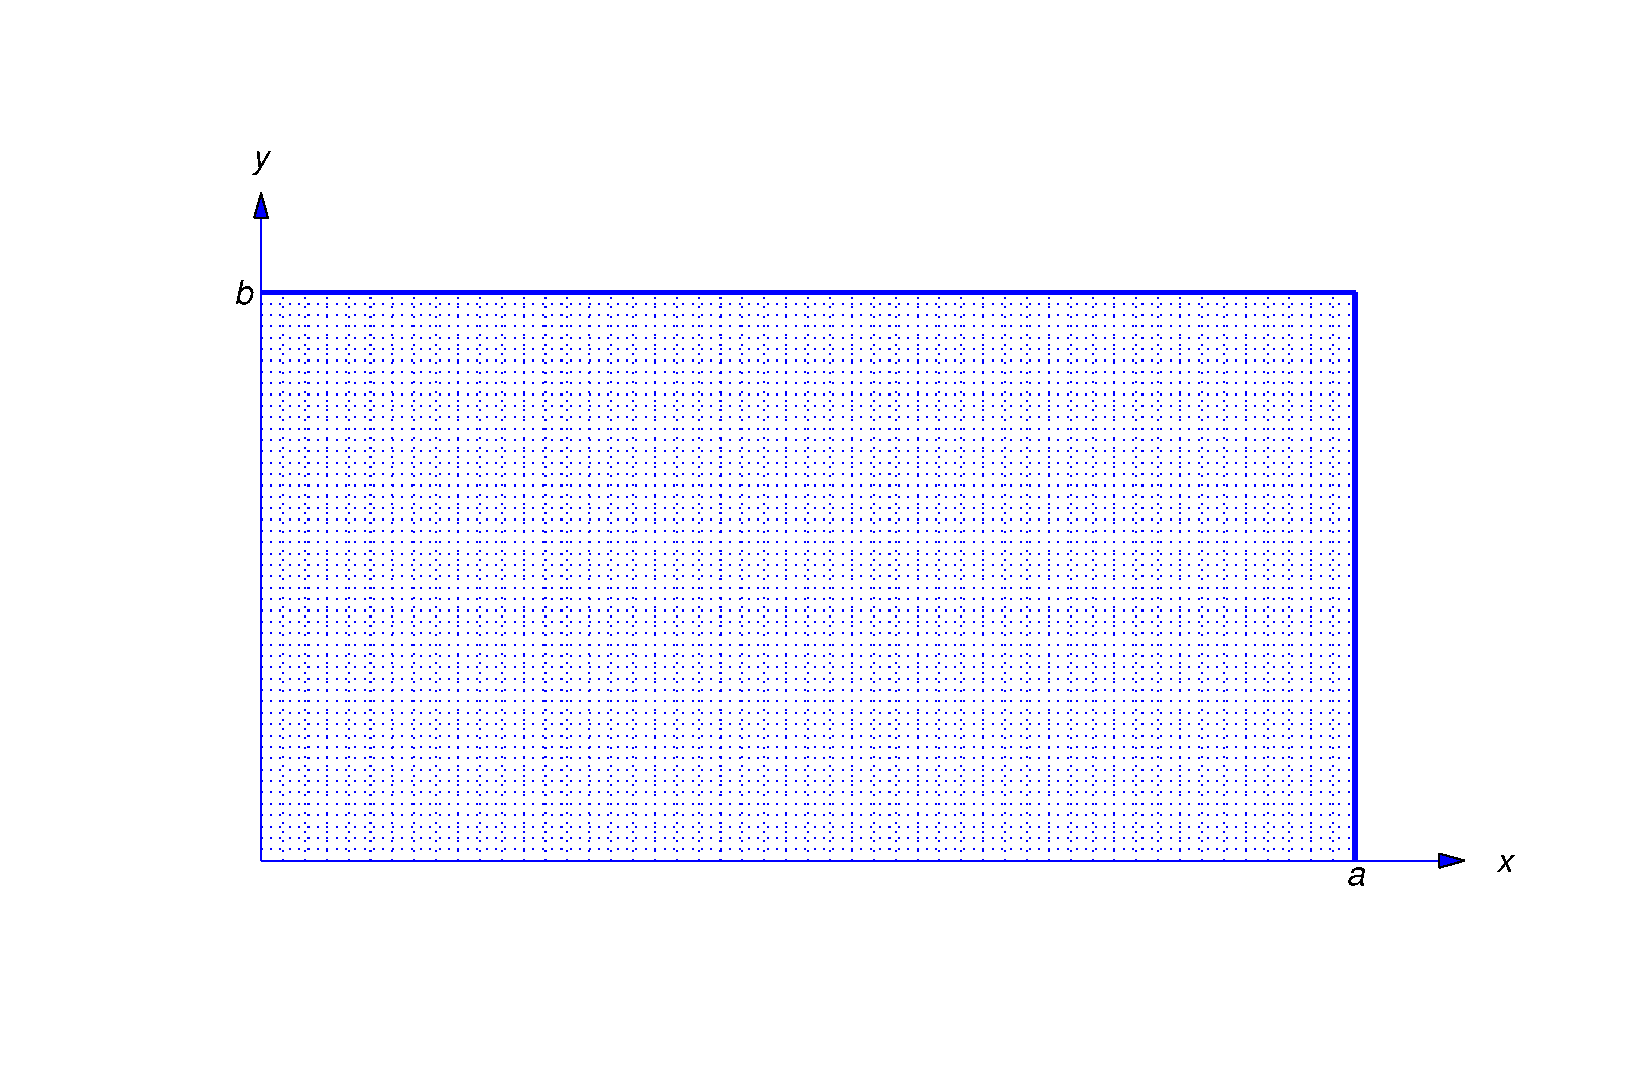
\includegraphics[bb=-78 148 689 643,width=5.67in,height=3.66in,keepaspectratio]{fig120301}
\caption{ A rectangular region and its boundary}
  \label{figure:12.3.1}
\end{figure}

The possible boundary conditions for this region can be written
as
$$
\begin{array}{lcllll}
(1-\alpha)u(x,0)&+&\alpha u_y(x,0)&=&f_0(x),  &0\le x\le
a,\\[2\jot]
(1-\beta) u(x,b)&+&\beta u_y(x,b)&=&f_1(x), &0\le x\le a,\\[2\jot]
(1-\gamma) u(0,y)&+&\gamma u_x(0,y)&=&g_0(y), &0\le y\le b,\\[2\jot]
(1-\delta) u(a,y)&+&\delta u_x(a,y)&=&g_1(y), &0\le y\le b,
\end{array}
$$
where $\alpha$, $\beta$, $\gamma$, and $\delta$  can each be either
$0$ or $1$;   thus, there are 16 possibilities.
Let
BVP$(\alpha,\beta,\gamma,\delta)(f_0,f_1,g_0,g_1)$
denote the problem of finding a solution of \eqref{eq:12.3.2} that
satisfies these conditions.
This is a Dirichlet problem if
$$
\alpha=\beta=\gamma=\delta=0
$$
(Figure~\ref{figure:12.3.2}),
or a Neumann problem if
$$
\alpha=\beta=\gamma=\delta=1
$$
(Figure~\ref{figure:12.3.3}).
The other 14 problems  are mixed.

\begin{figure}[htbp]
\color{blue}
  \begin{minipage}[b]{0.5\linewidth}
    \centering
   \scalebox{.5}{
  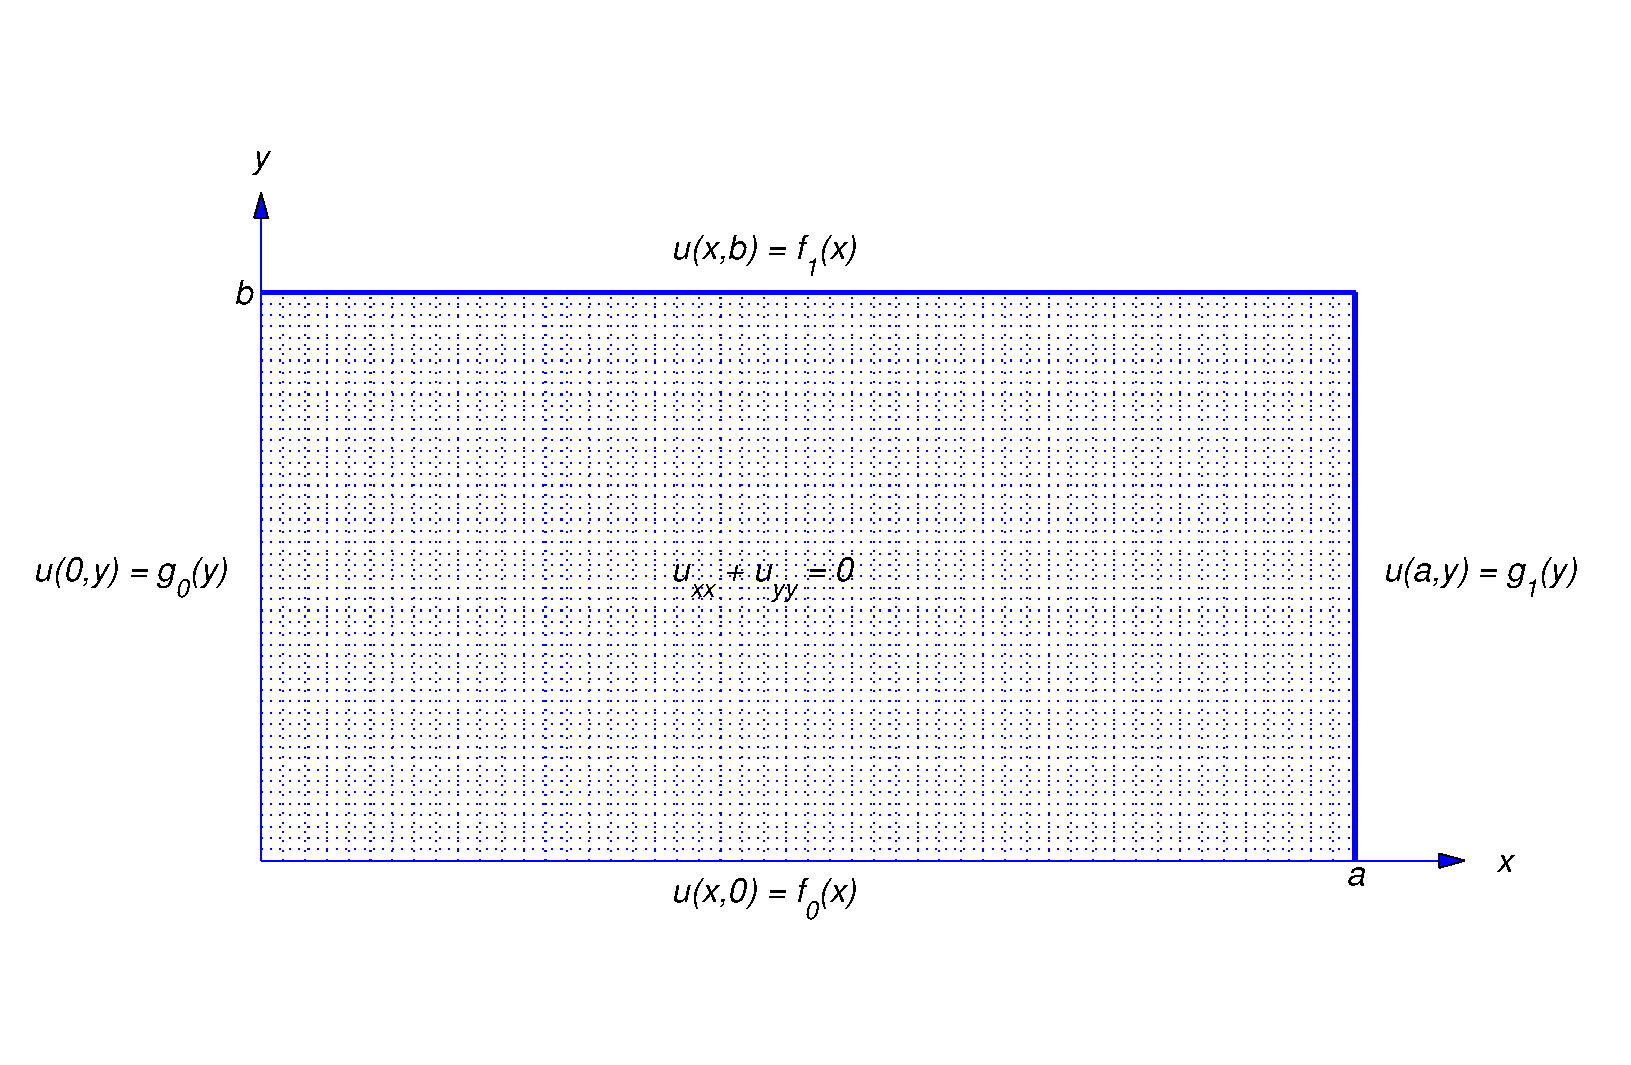
\includegraphics[bb=-78 148 689 643,width=5.67in,height=3.66in,keepaspectratio]{fig120302}}
\caption{ A Dirichlet problem}
  \label{figure:12.3.2}
\end{minipage}
  \begin{minipage}[b]{0.5\linewidth}
    \centering
   \scalebox{.5}{
  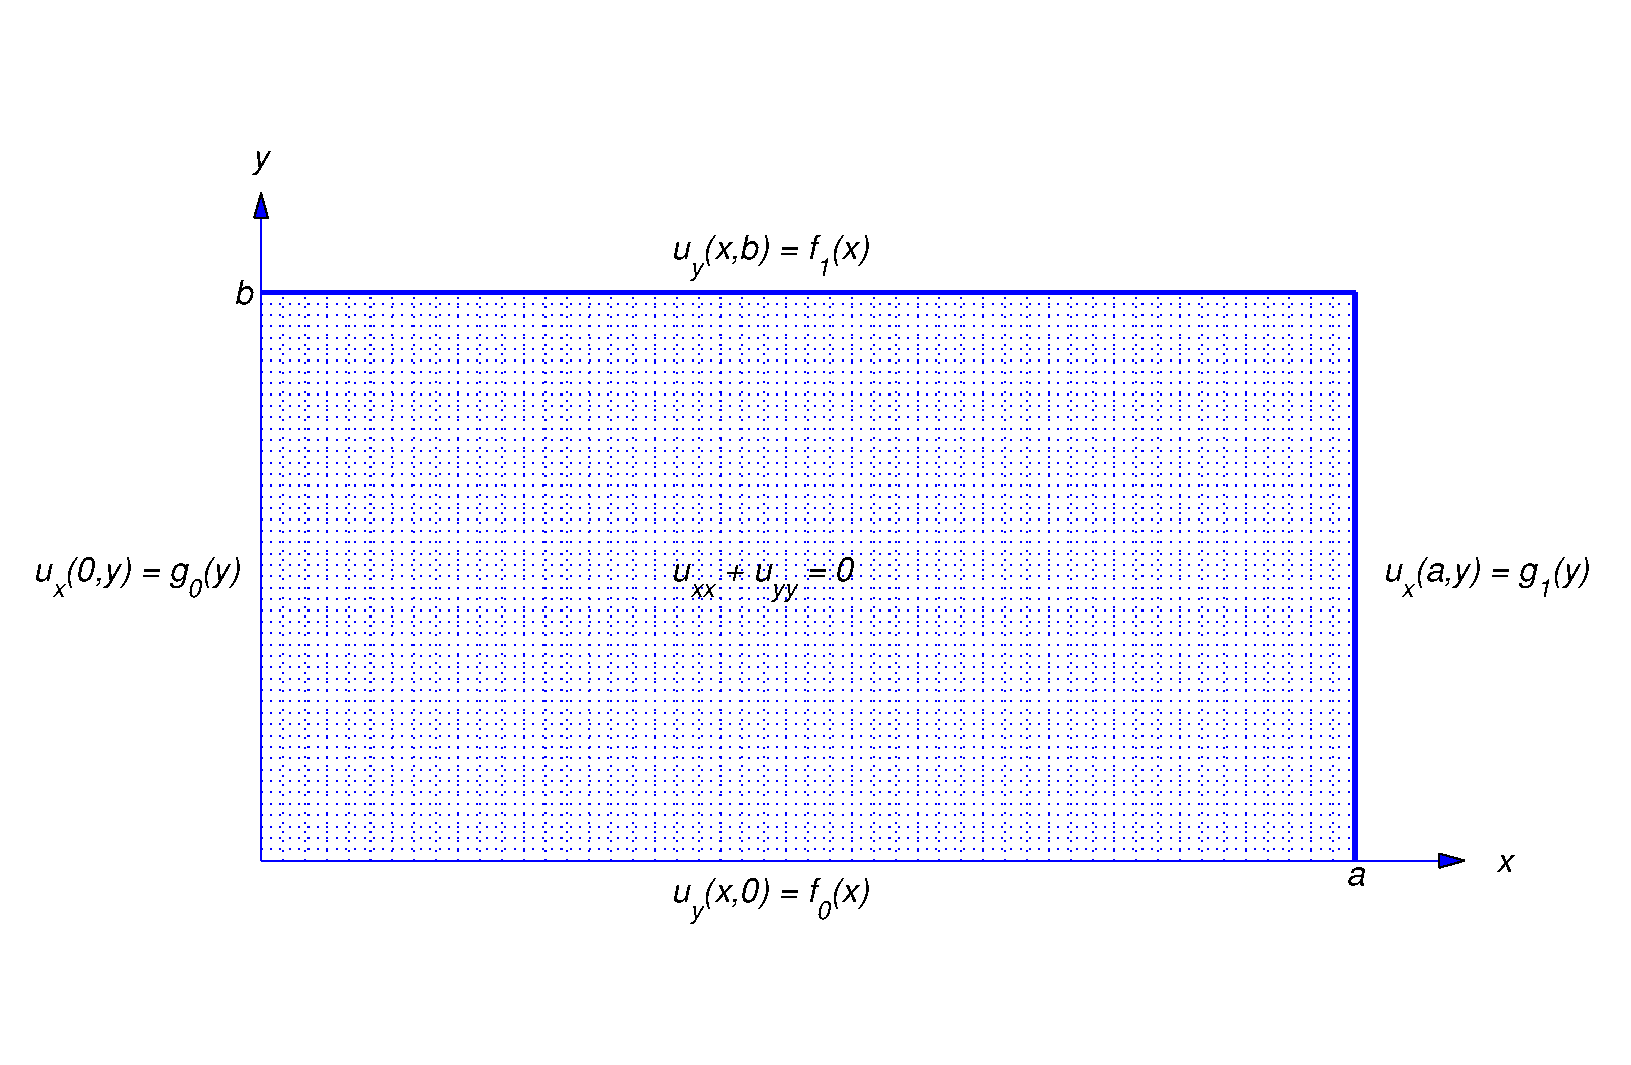
\includegraphics[bb=-78 148 689 643,width=5.67in,height=3.66in,keepaspectratio]{fig120303}}
\caption{ A Neumann problem}
  \label{figure:12.3.3}
\end{minipage}
\end{figure}

For given $(\alpha,\beta,\gamma,\delta)$, the sum of
solutions of
$$
\mbox{BVP}(\alpha,\beta,\gamma,\delta)(f_0,0,0,0),\quad
\mbox{BVP}(\alpha,\beta,\gamma,\delta)(0,f_1,0,0),
$$
$$
\mbox{BVP}(\alpha,\beta,\gamma,\delta)(0,0,g_0,0),
\mbox{\quad and \quad}
\mbox{BVP}(\alpha,\beta,\gamma,\delta)(0,0,0,g_1)
$$
is a solution of
$$
\mbox{BVP}(\alpha,\beta,\gamma,\delta)(f_0,f_1,g_0,g_1).
$$
 Therefore we  concentrate
on problems where only one of the functions $f_0$,
$f_1$,
$g_0$, $g_2$ isn't  identically zero. There are 64 (count them!)
 problems of this form. Each has homogeneous
boundary conditions on three sides of the rectangle, and a
nonhomogeneous boundary condition on the fourth. We  use
separation of variables to find infinitely many functions
that satisfy
Laplace's equation and the three homogeneous boundary
conditions in the open rectangle.
 We then use
these solutions as  building blocks to construct a formal solution of
Laplace's equation that also  satisfies the  nonhomogeneous
boundary condition.
Since it's not feasible to consider
all 64 cases, we'll restrict our attention in the text to
just four.  Others are discussed in the exercises.

If $v(x,y)=X(x)Y(y)$ then $$ v_{xx}+v_{yy}=X''Y+XY''=0 $$ for all
$(x,y)$ if and only if $$ {X''\over X}=-{Y''\over Y}=k $$ for all
$(x,y)$, where $k$ is a separation constant. This equation is
equivalent to
\begin{equation} \label{eq:12.3.3}
X''-kX=0,\quad  Y''+kY=0.
\end{equation}
From here,
the strategy  depends upon the
boundary conditions. We  illustrate this by examples.

\begin{example}\label{example:12.3.1} \rm
Define the formal solution of
\begin{equation} \label{eq:12.3.4}
\begin{array}{c}
u_{xx}+u_{yy}=0,\quad 0<x<a,\quad  0<y<b,\\
u(x,0)=f(x),\quad u(x,b)=0,\quad 0\le x\le a,\\
u(0,y)=0,\quad u(a,y)=0,\quad 0\le y\le b
\end{array}
\end{equation}
(Figure~\ref{figure:12.3.4}).
\end{example}

\begin{figure}[tbp]
  \centering\color{blue}
  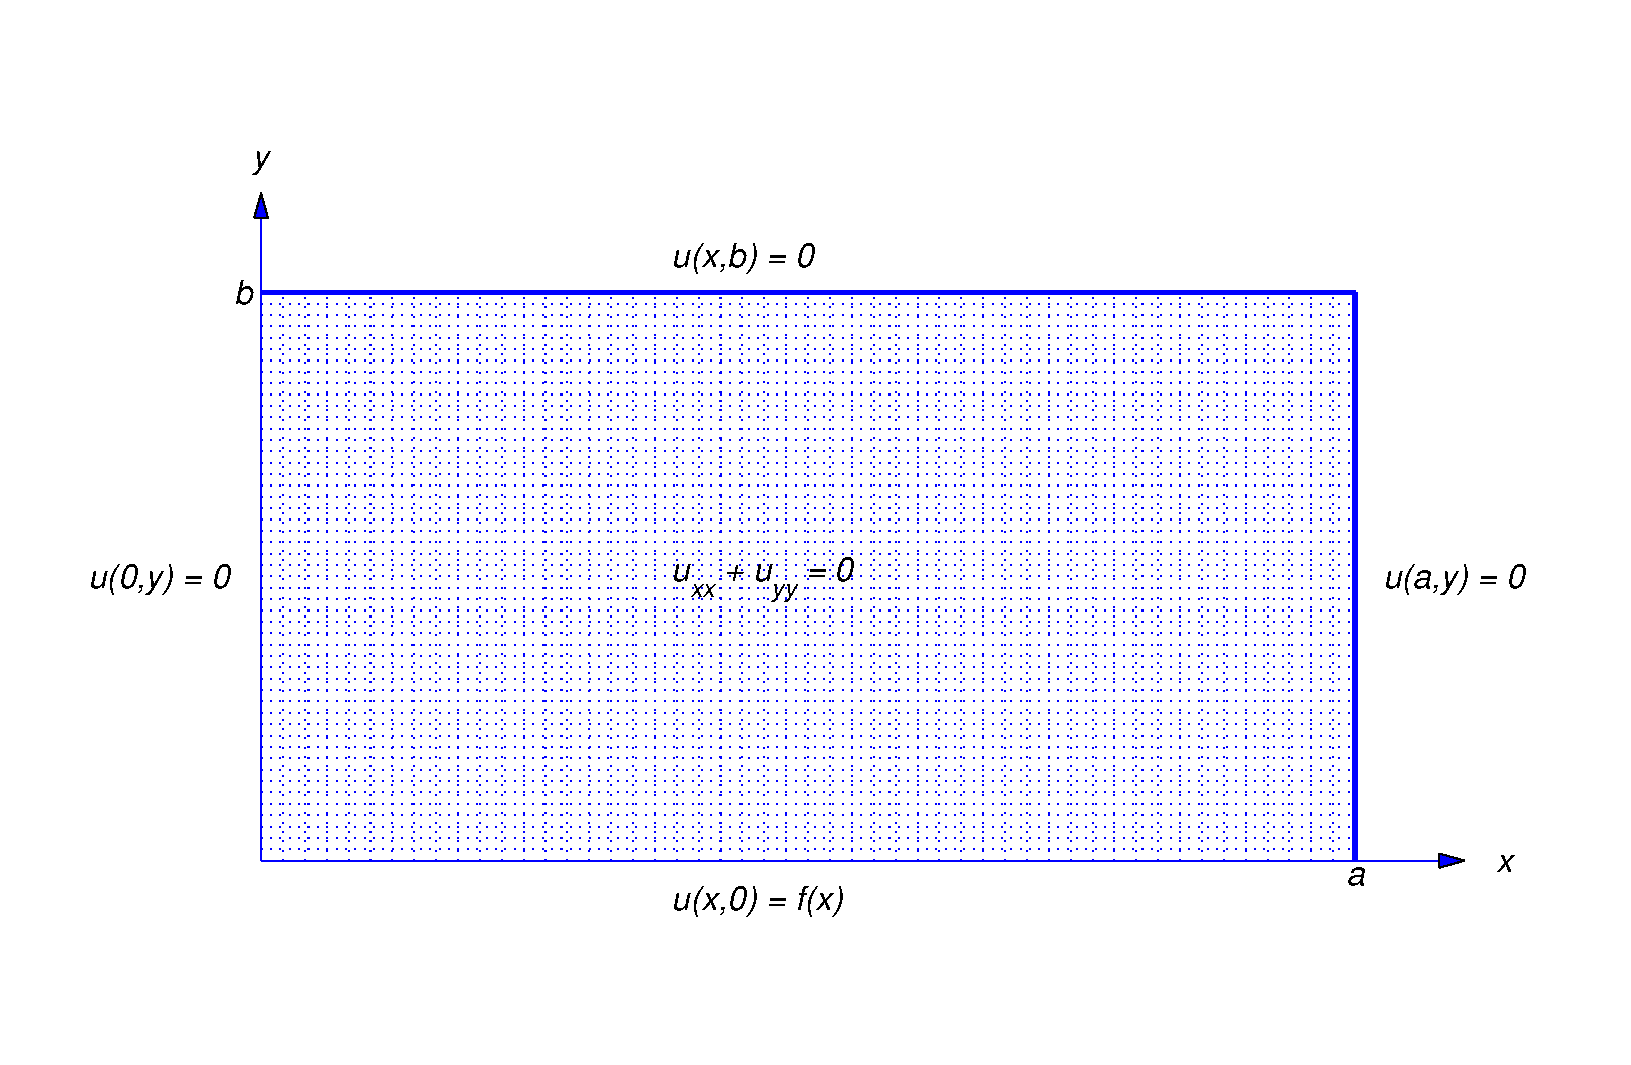
\includegraphics[bb=-78 148 689 643,width=5.67in,height=3.66in,keepaspectratio]{fig120304}
\caption{ The boundary value problem \eqref{eq:12.3.4}}
  \label{figure:12.3.4}
\end{figure}

\solution
The boundary conditions in \eqref{eq:12.3.4} require
 products $v(x,y)=X(x)Y(y)$ such that
$X(0)=X(a)=Y(b)=0$; hence, we let $k=-\lambda$ in \eqref{eq:12.3.3}.
Thus, $X$ and $Y$ must satisfy
\begin{equation} \label{eq:12.3.5}
X''+\lambda X=0,\quad X(0)=0,\quad X(a)=0
\end{equation}
and
\begin{equation} \label{eq:12.3.6}
Y''-\lambda Y=0,\quad Y(b)=0.
\end{equation}
 From Theorem~\ref{thmtype:11.1.2}, the eigenvalues of \eqref{eq:12.3.5}
are $\lambda_n=n^2\pi^2/a^2$, with
associated eigenfunctions
$$
X_n=\sin{n\pi x\over a}, \quad n=1,2,3,\dots.
$$
Substituting $\lambda=n^2\pi^2/a^2$  into
\eqref{eq:12.3.6} yields
$$
Y''-(n^2\pi^2/a^2)Y=0,\quad Y(b)=0,
$$
so we could take
\begin{equation} \label{eq:12.3.7}
Y_n=\sinh{n\pi(b-y)\over a};
\end{equation}
however, because of the nonhomogeneous Dirichlet  condition at $y=0$,
it's better to require that
$Y_n(0)=1$, which can be achieved by  dividing the right side
of
\eqref{eq:12.3.7} by its value at $y=0$;   thus, we take
$$
Y_n={\sinh n\pi(b-y)/a\over\sinh n\pi b/a}.
$$
Then
$$
v_n(x,y)=X_n(x)Y_n(y)={\sinh n\pi(b-y)/a\over\sinh n\pi b/a}\sin{n\pi
x\over a},
$$
so $v_n(x,0)=\sin n\pi x/a$ and
 $v_n$ satisfies \eqref{eq:12.3.4} with $f(x)=\sin n\pi x/a$. More
generally,
 if $\alpha_1$, \dots, $\alpha_m$ are arbitrary constants
then
$$
u_m(x,y)=\sum_{n=1}^m\alpha_n
{\sinh n\pi(b-y)/a\over\sinh n\pi b/a}
\sin{n\pi x\over a}
$$
satisfies \eqref{eq:12.3.4} with
$$
f(x)=\sum_{n=1}^m\alpha_n\sin{n\pi x\over L}.
$$
Therefore, if $f$ is an arbitrary piecewise smooth function on
$[0,a]$,  we define the formal solution of \eqref{eq:12.3.4} to be
\begin{equation} \label{eq:12.3.8}
u(x,y)=\sum_{n=1}^\infty \alpha_n
{\sinh n\pi(b-y)/a\over\sinh n\pi b/a}
\sin{n\pi x\over a},
\end{equation}
where
$$
S(x)=\sum_{n=1}^\infty \alpha_n\sin{n\pi x\over a}
$$
is the Fourier sine series of $f$ on $[0,a]$; that is,
$$
\alpha_n={2\over a}\int_0^af(x)\sin{n\pi x\over a}\,dx,\quad
n=1,2,3,\dots.
\eqno{\bbox}
$$

If $y<b$ then
\begin{equation} \label{eq:12.3.9}
{\sinh n\pi(b-y)/a\over\sinh n\pi b/a}\approx e^{-n\pi y/a}
\end{equation}
for large $n$,
so the series in \eqref{eq:12.3.8} converges if $0< y < b$;
 moreover, since also
$$
{\cosh n\pi(b-y)/a\over\sinh n\pi b/a}\approx e^{-n\pi y/a}
$$
for large $n$, Theorem~\ref{thmtype:12.1.2}
 applied twice with
 $z=x$ and  twice with  $z=t$, shows that   $u_{xx}$  and $u_{yy}$
can be obtained by differentiating $u$ term by term if $0<y<b$.
 (Exercise~\ref{exer:12.3.37}). Therefore $u$
satisfies Laplace's equation in the interior of the rectangle
in Figure~\ref{figure:12.3.4}.
Moreover, the series in \eqref{eq:12.3.8}
also converges on the boundary of the rectangle, and satisfies
the three homogeneous boundary conditions
conditions in \eqref{eq:12.3.4}.
 Therefore, since $u(x,0)=S(x)$ for $0\le x\le
L$, $u$ is an actual solution of \eqref{eq:12.3.5} if and only if
$S(x)=f(x)$ for $0\le x\le a$.
From Theorem~\ref{thmtype:11.3.2}, this is true if $f$
is continuous and piecewise smooth on $[0,L]$,
and $f(0)=f(L)=0$.

\begin{example}\label{example:12.3.2} \rm
Solve \eqref{eq:12.3.4} with $f(x)=x(x^2-3ax+2a^2)$.
\end{example}

\solution  From Example~\ref{example:11.3.6},
$$
S(x)={12a^3\over\pi^3}\sum_{n=1}^\infty{1\over n^3}\sin{n\pi
x\over a}.
$$
Therefore
\begin{equation} \label{eq:12.3.10}
u(x,y)={12a^3\over\pi^3}\sum_{n=1}^\infty{\sinh n\pi(b-y)/a\over
n^3\sinh n\pi b/a}
\sin{n\pi x\over a}.
\end{equation}

To compute approximate values of $u(x,y)$, we must use partial sums of
the form
$$
u_m(x,y)={12a^3\over\pi^3}\sum_{n=1}^m{\sinh n\pi(b-y)/a\over
n^3\sinh n\pi b/a}
\sin{n\pi x\over a}.
$$
Because of \eqref{eq:12.3.9}, small values of $m$
provide  sufficient accuracy for most applications if $0<y<b$.
Moreover, the
$n^3$ in the denominator in \eqref{eq:12.3.10} ensures that this is also
true for $y=0$.
 For graphing purposes, we chose $a=2$, $b=1$,
and $m=10$.
Figure~\ref{figure:12.3.5}  shows the surface
$$
u=u(x,y),\quad 0\le x\le 2,\quad 0\le y\le1,
$$
while Figure~\ref{figure:12.3.6}  shows the curves
$$
u=u(x,0.1k),\quad 0\le x\le2,\quad k=0,1,\dots,10.
$$

\begin{figure}[H]
\color{blue}
  \begin{minipage}[b]{0.5\linewidth}
    \centering
   \scalebox{.65}{
  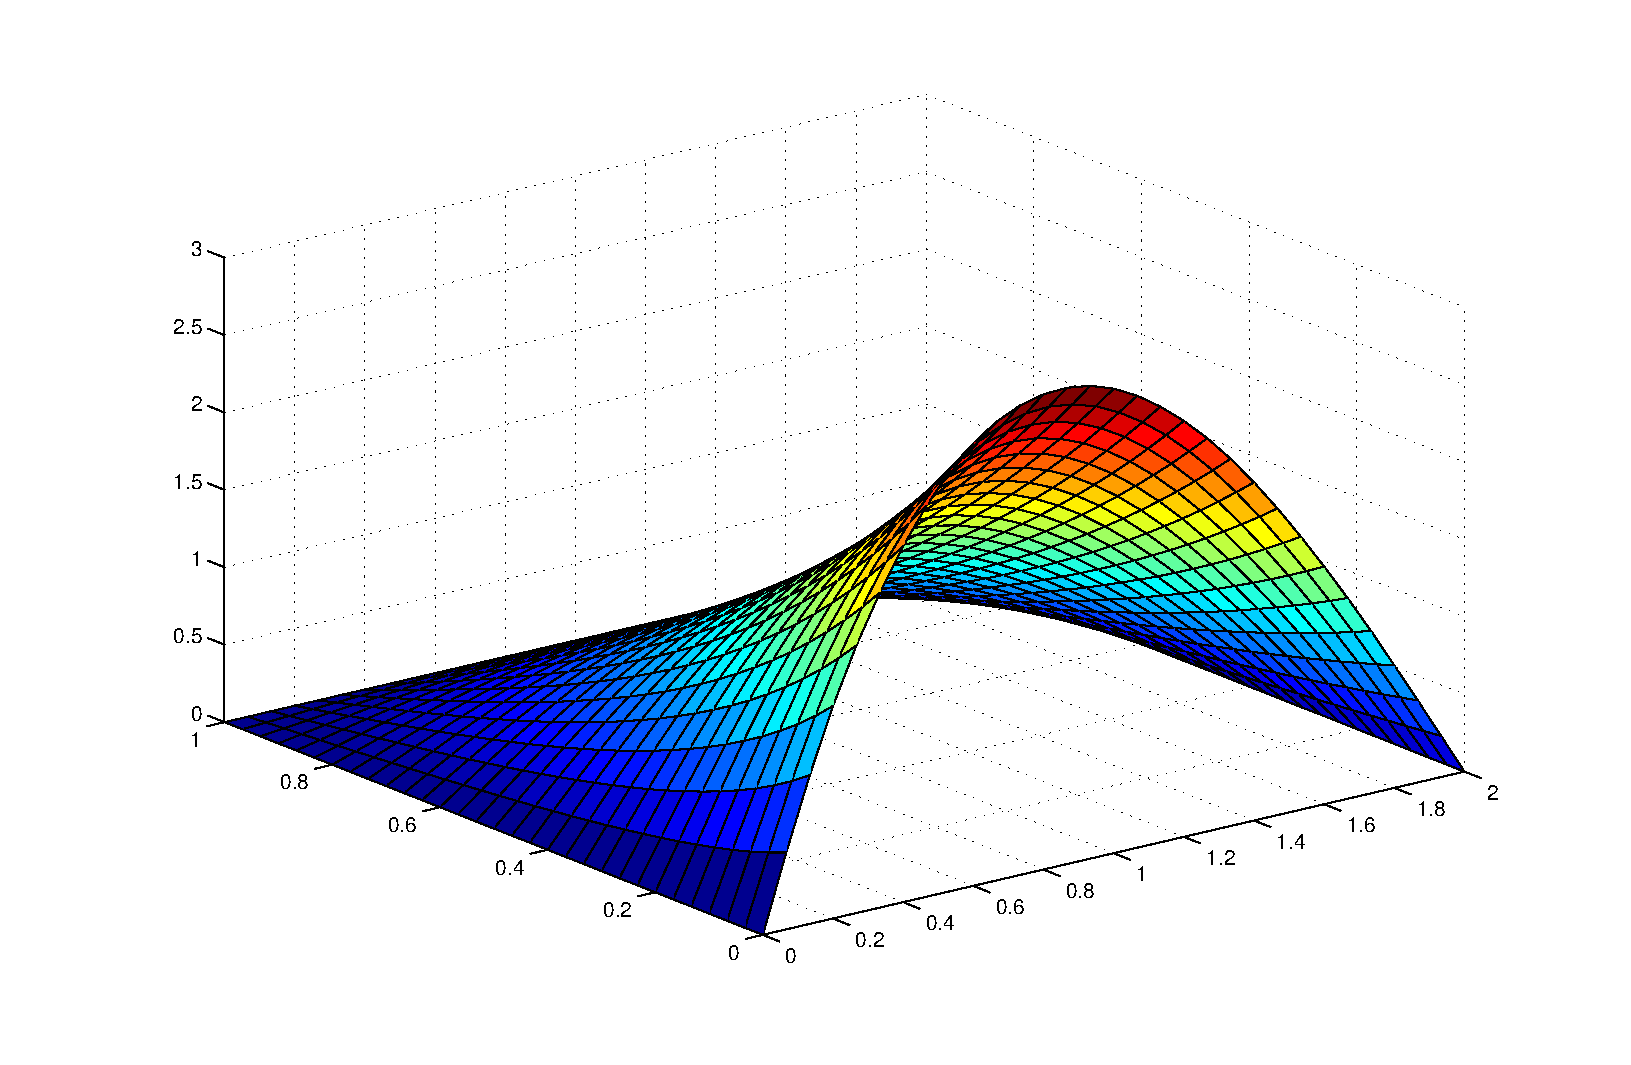
\includegraphics[bb=-78 148 689 643,width=5.67in,height=3.66in,keepaspectratio]{fig120305}}
  \caption{}
  \label{figure:12.3.5}
\end{minipage}
  \begin{minipage}[b]{0.5\linewidth}
    \centering
   \scalebox{.65}{
  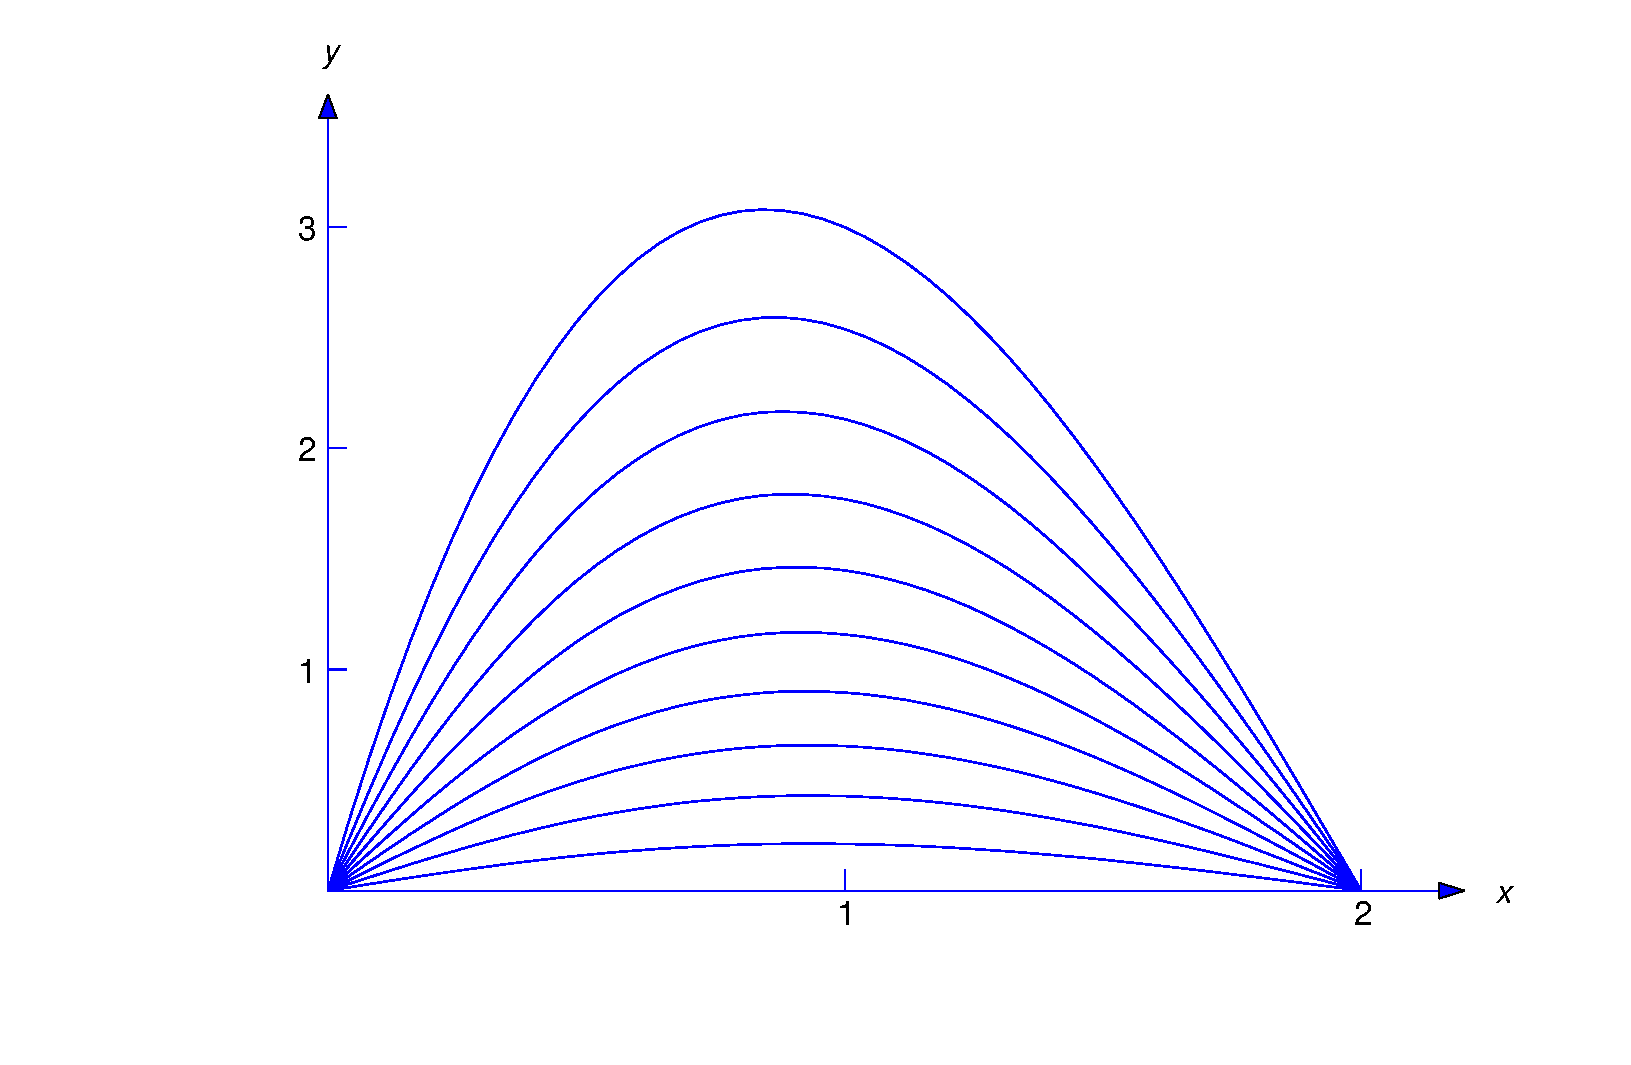
\includegraphics[bb=-78 148 689 643,width=5.67in,height=3.66in,keepaspectratio]{fig120306}}
  \caption{}
  \label{figure:12.3.6}
\end{minipage}
\end{figure}

\begin{example}\label{example:12.3.3}    \rm
Define the formal solution of
\begin{equation} \label{eq:12.3.11}
\begin{array}{c}
u_{xx}+u_{yy}=0,\quad 0<x<a,\quad  0<y<b,\\
u(x,0)=0,\quad u_y(x,b)=f(x),\quad 0\le x\le a,\\
u_x(0,y)=0,\quad u_x(a,y)=0,\quad 0\le y\le b
\end{array}
\end{equation}
(Figure~\ref{figure:12.3.7}).
\end{example}

\begin{figure}[H]
  \centering\color{blue}
  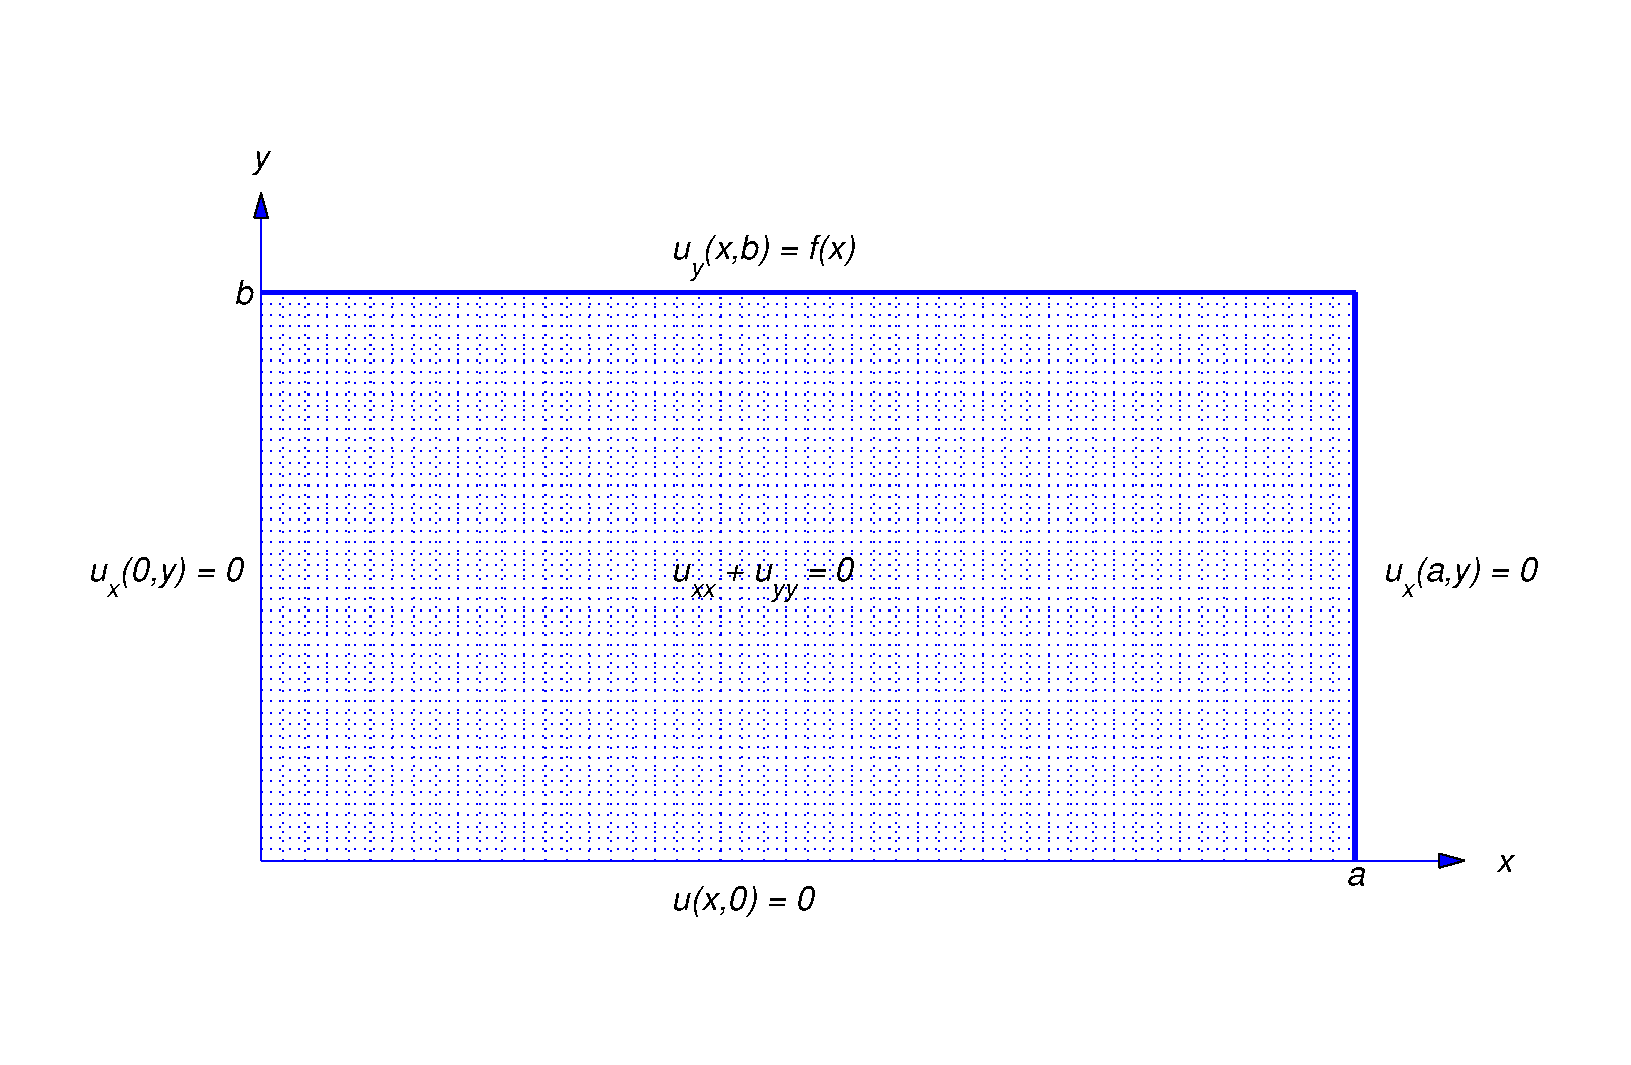
\includegraphics[bb=-78 148 689 643,width=5.67in,height=3.66in,keepaspectratio]{fig120307}
\caption{ The boundary value problem \eqref{eq:12.3.11}}
  \label{figure:12.3.7}
\end{figure}

\solution
The boundary conditions in \eqref{eq:12.3.11} require
 products $v(x,y)=X(x)Y(y)$ such that
$X'(0)=X'(a)=Y(0)=0$; hence, we let $k=-\lambda$ in
\eqref{eq:12.3.3}. Thus, $X$ and $Y$ must satisfy
\begin{equation} \label{eq:12.3.12}
X''+\lambda X=0,\quad X'(0)=0,\quad X'(a)=0
\end{equation}
and
\begin{equation} \label{eq:12.3.13}
Y''-\lambda Y=0,\quad Y(0)=0.
\end{equation}
 From Theorem~\ref{thmtype:11.1.3}, the eigenvalues of \eqref{eq:12.3.12}
are $\lambda=0$, with associated
eigenfunction $X_0=1$, and $\lambda_n=n^2\pi^2/a^2$, with
associated eigenfunctions
$$
X_n=\cos{n\pi x\over a}, \quad n=1,2,3,\dots.
$$
Since $Y_0=y$ satisfies \eqref{eq:12.3.13} with $\lambda=0$,
we take $v_0(x,y)=X_0(x)Y_0(y)= y$.
Substituting $\lambda=n^2\pi^2/a^2$  into
\eqref{eq:12.3.13} yields
$$
Y''-(n^2\pi^2/a^2)Y=0,\quad Y(0)=0,
$$
so we could take
\begin{equation} \label{eq:12.3.14}
Y_n=\sinh{n\pi y\over a}.
\end{equation}
However, because of the nonhomogeneous Neumann condition at $y=b$, it's
better to require that
$Y_n'(b)=1$, which can be achieved by  dividing the right side
of
\eqref{eq:12.3.14} by the value of its derivative  at $y=b$; thus,
$$
Y_n={a\sinh n\pi y/a\over n\pi\cosh n\pi b/a}.
$$
Then
$$
v_n(x,y)=X_n(x)Y_n(y)=
{a\sinh n\pi y/a\over n\pi\cosh n\pi b/a}\cos{n\pi x\over a},
$$
so
$$
{\partial v_n\over \partial y}(x,b)=\cos{n\pi x\over a}.
$$
Therefore
 $v_n$ satisfies \eqref{eq:12.3.11} with $f(x)=\cos n\pi x/a$. More
generally,
 if $\alpha_0$, \dots, $\alpha_m$ are arbitrary constants
then
$$
u_m(x,y)=\alpha_0y+{a\over\pi}\sum_{n=1}^m\alpha_n
{\sinh n\pi y/a\over n\cosh n\pi b/a}
\cos{n\pi x\over a}
$$
satisfies \eqref{eq:12.3.11} with
$$
f(x)=\alpha_0+\sum_{n=1}^m\alpha_n\cos{n\pi x\over L}.
$$
Therefore, if $f$ is an arbitrary piecewise smooth function on
$[0,a]$  we define the formal solution of \eqref{eq:12.3.11} to be
$$
u(x,y)=\alpha_0y+{a\over\pi}\sum_{n=1}^\infty \alpha_n
{\sinh n\pi y/a\over n\cosh n\pi b/a}
\cos{n\pi x\over a},
$$
where
$$
C(x)=\alpha_0+\sum_{n=1}^\infty \alpha_n\cos{n\pi x\over a}
$$
is the Fourier cosine series of $f$ on $[0,a]$; that is,
$$
\alpha_0={1\over a}\int_0^af(x)\,dx
\mbox{\quad and \quad}
\alpha_n={2\over a}\int_0^af(x)\cos{n\pi x\over a}\,dx,\quad
n=1,2,3,\dots.
$$

\begin{example}\label{example:12.3.4}\rm
Solve \eqref{eq:12.3.11} with $f(x)=x$.
\end{example}

\solution From Example~\ref{example:11.3.1},
$$
C(x)=\dst{a\over2}-{4a\over\pi^2}\sum_{n=1}^\infty{1\over(2n-1)^2}
\cos{(2n-1)\pi x\over a}.
$$
Therefore
\begin{equation} \label{eq:12.3.15}
u(x,y)=\dst{ay\over2}-{4a^2\over\pi^3}\sum_{n=1}^\infty
{\sinh(2n-1)\pi y/a\over(2n-1)^3\cosh(2n-1)\pi b/a}
\cos{(2n-1)\pi x\over a}.
\end{equation}
 For graphing purposes, we chose $a=2$, $b=1$,
and retained the terms through $n=10$ in  \eqref{eq:12.3.15}.
Figure~\ref{figure:12.3.8}  shows the surface
$$
u=u(x,y),\quad 0\le x\le 2,\quad 0\le y\le1,
$$
while Figure~\ref{figure:12.3.9}  shows the curves
$$
u=u(x,.1k),\quad 0\le x\le2,\quad k=0,1,\dots,10.
$$

\begin{figure}[H]
\color{blue}
  \begin{minipage}[b]{0.5\linewidth}
    \centering
   \scalebox{.65}{
  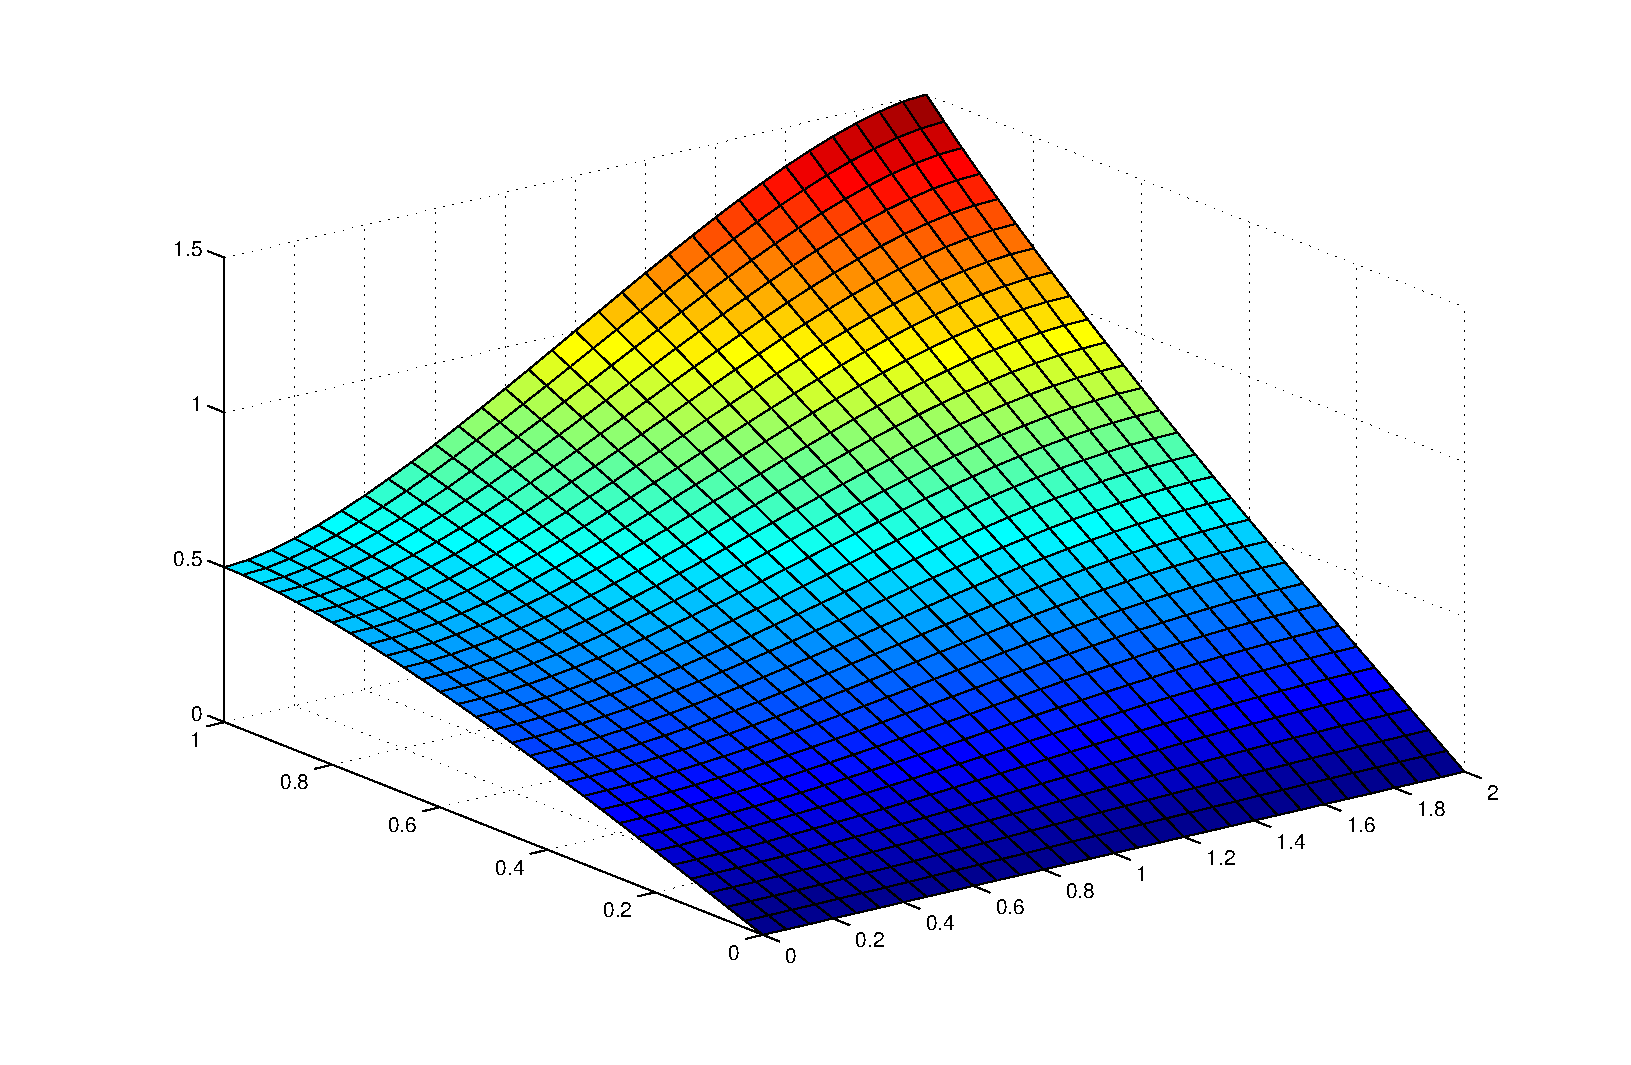
\includegraphics[bb=-78 148 689 643,width=5.67in,height=3.66in,keepaspectratio]{fig120308}}
  \caption{}
  \label{figure:12.3.8}
\end{minipage}
  \begin{minipage}[b]{0.5\linewidth}
    \centering
   \scalebox{.65}{
  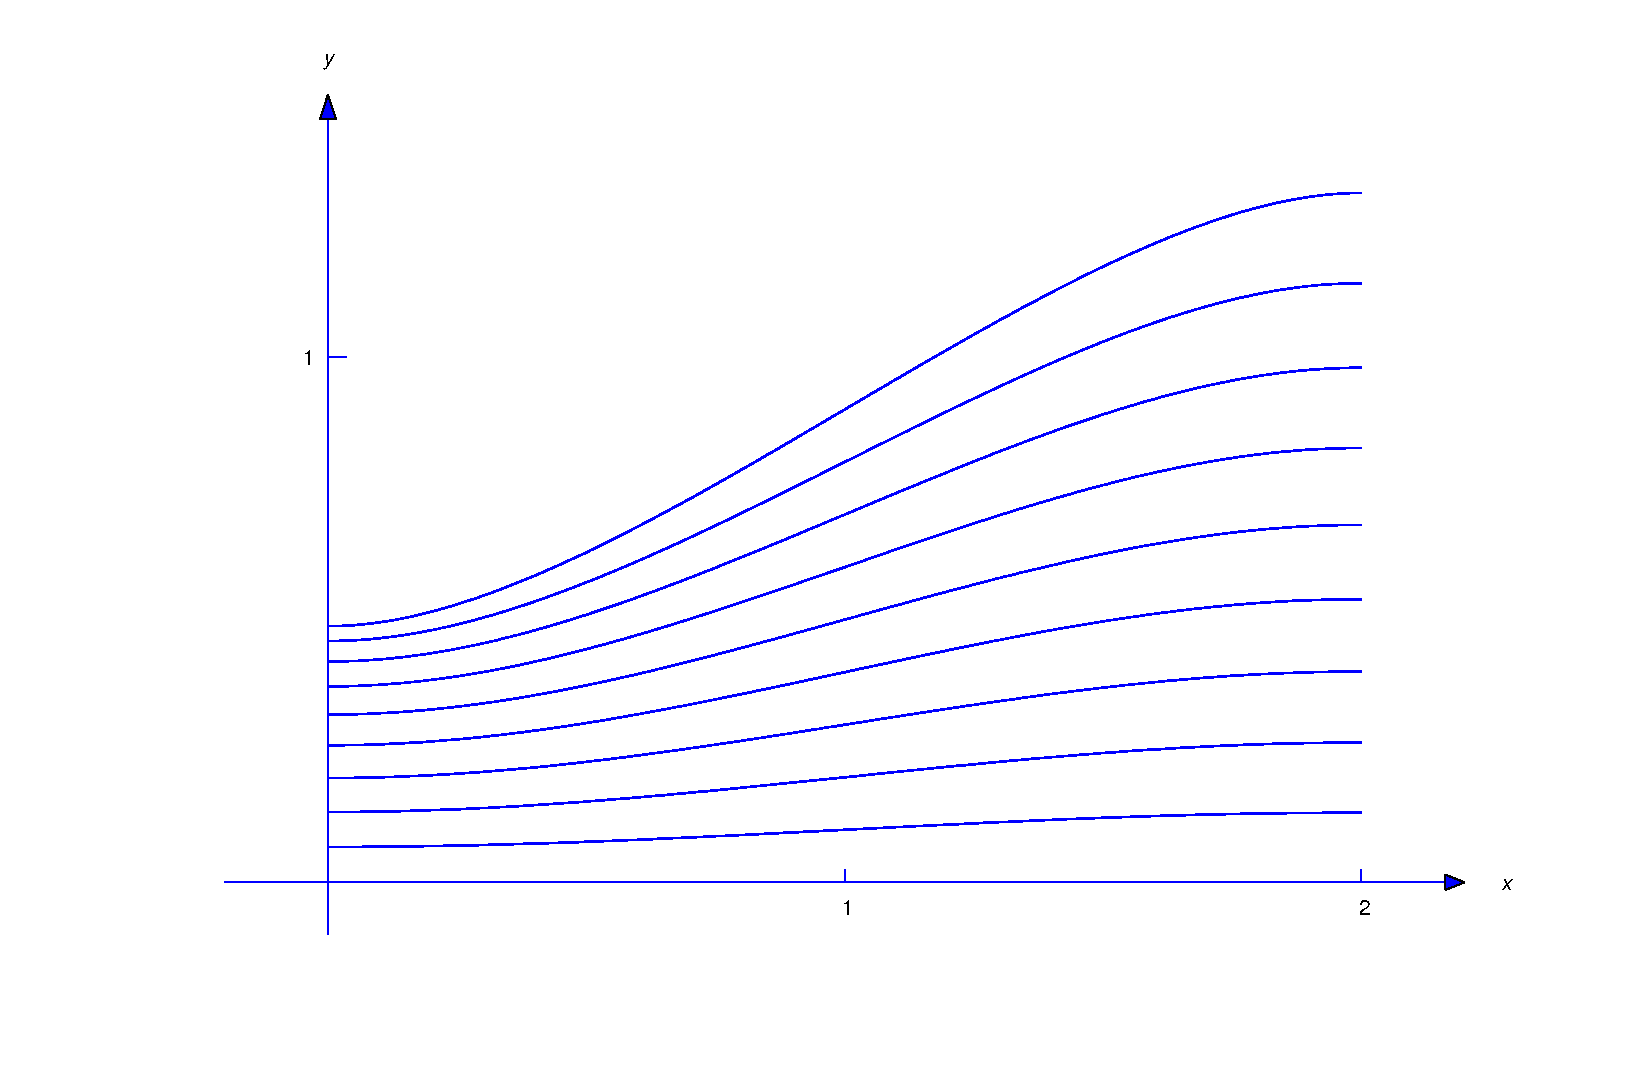
\includegraphics[bb=-78 148 689 643,width=5.67in,height=3.66in,keepaspectratio]{fig120309}}
  \caption{}
  \label{figure:12.3.9}
\end{minipage}
\end{figure}

\begin{example}\label{example:12.3.5} \rm
Define the formal solution of
\begin{equation} \label{eq:12.3.16}
\begin{array}{c}
u_{xx}+u_{yy}=0,\quad 0<x<a,\quad  0<y<b,\\
u(x,0)=0,\quad u_y(x,b)=0,\quad 0\le x\le a,\\
u(0,y)=g(y),\quad u_x(a,y)=0,\quad 0\le y\le b
\end{array}
\end{equation}
(Figure~\ref{figure:12.3.10}).
\end{example}

\begin{figure}[tbp]
  \centering\color{blue}
  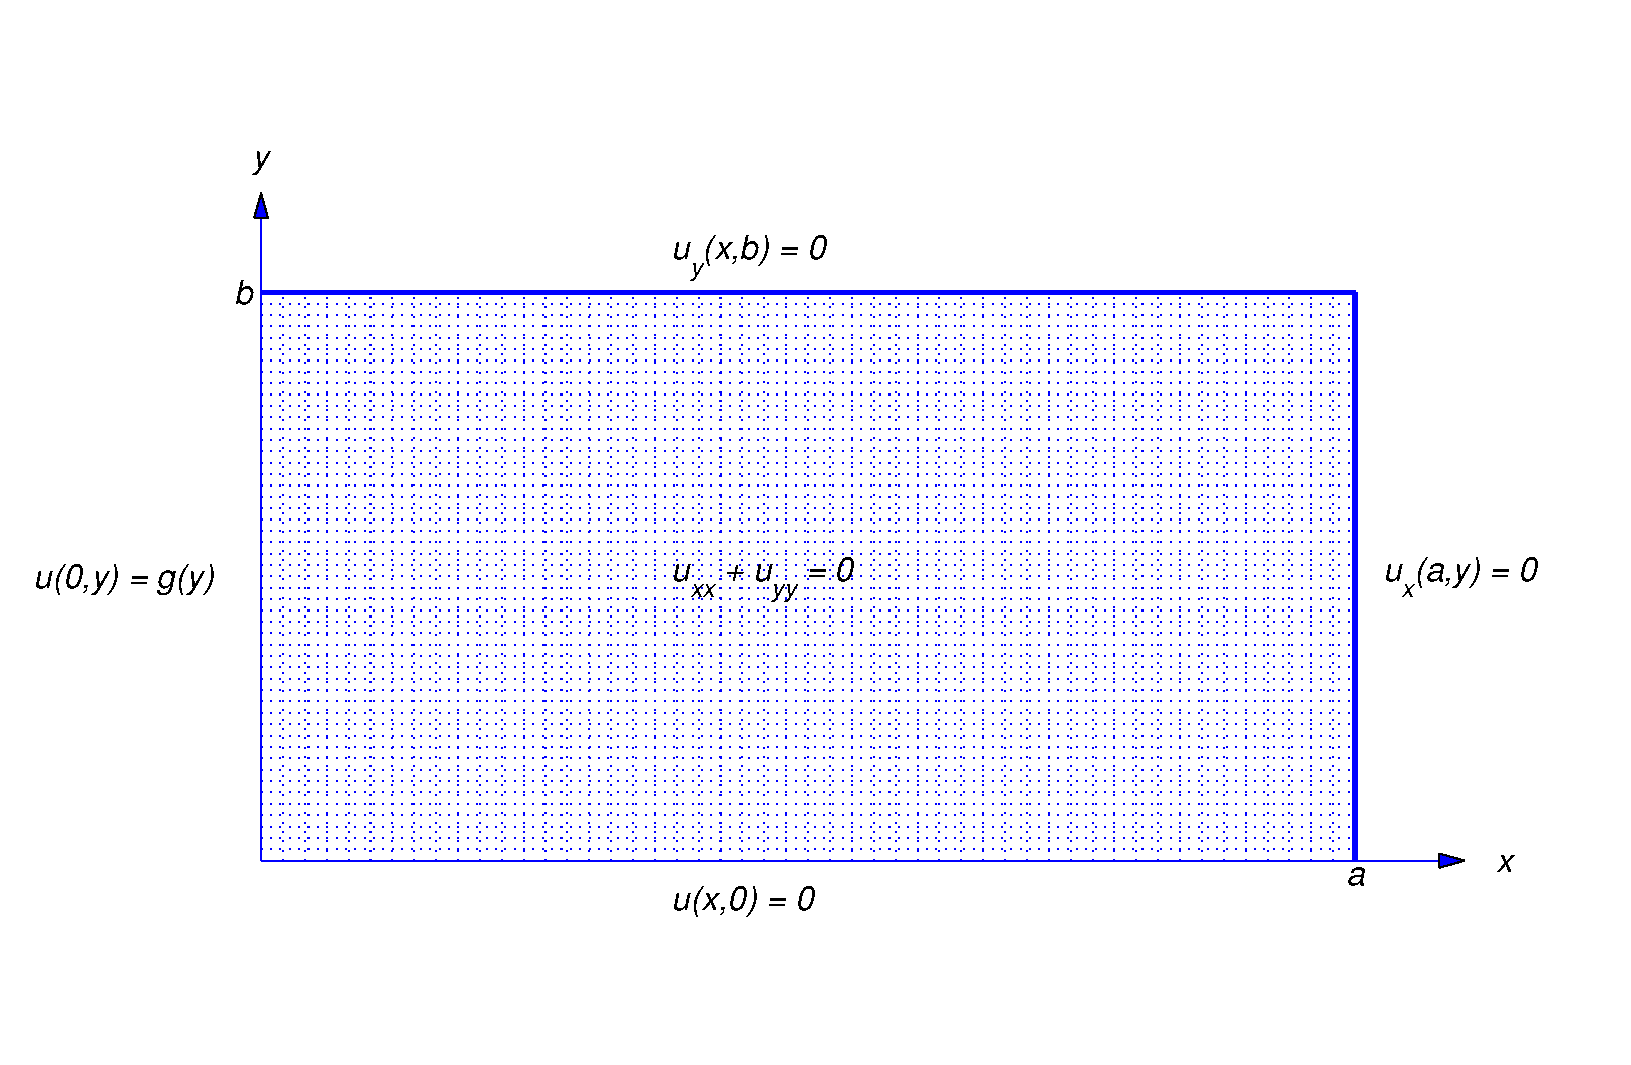
\includegraphics[bb=-78 148 689 643,width=5.67in,height=3.66in,keepaspectratio]{fig120310}
\caption{ The boundary value problem \eqref{eq:12.3.16}}
  \label{figure:12.3.10}
\end{figure}

\solution
The boundary conditions in \eqref{eq:12.3.16} require
 products $v(x,y)=X(x)Y(y)$ such that
$Y(0)=Y'(b)=X'(a)=0$; hence, we let $k=\lambda$ in
\eqref{eq:12.3.3}. Thus, $X$ and $Y$ must satisfy
\begin{equation} \label{eq:12.3.17}
X''-\lambda X=0,\quad \quad X'(a)=0
\end{equation}
and
\begin{equation} \label{eq:12.3.18}
Y''+\lambda Y=0,\quad Y(0)=0,\quad Y'(b)=0.
\end{equation}
 From Theorem~\ref{thmtype:11.1.4}, the eigenvalues of \eqref{eq:12.3.18}
are $\lambda_n=(2n-1)^2\pi^2/4b^2$, with
associated eigenfunctions
$$
Y_n=\sin{(2n-1)\pi y\over2b}, \quad n=1,2,3,\dots.
$$
Substituting $\lambda=(2n-1)^2\pi^2/4b^2$  into
\eqref{eq:12.3.17} yields
$$
X''-((2n-1)^2\pi^2/4b^2)X=0,\quad X'(a)=0,
$$
so we could take
\begin{equation} \label{eq:12.3.19}
X_n=\cosh{(2n-1)\pi(x-a)\over 2b}.
\end{equation}
However, because of the nonhomogeneous Dirichlet condition at $x=0$, it's
better to require that
$X_n(0)=1$, which can be achieved by  dividing the right side
of
\eqref{eq:12.3.19} by its  value  at $x=0$; thus,
$$
X_n=
{\cosh(2n-1)\pi(x-a)/2b\over\cosh(2n-1)\pi a/2b}.
$$
Then
$$
v_n(x,y)=X_n(x)Y_n(y)=
{\cosh(2n-1)\pi(x-a)/2b\over\cosh(2n-1)\pi a/2b}\sin{(2n-1)\pi
y\over2b},
$$
so
$$
v_n(0,y)=\sin{(2n-1)\pi y\over2b}.
$$
Therefore
 $v_n$ satisfies \eqref{eq:12.3.16} with $g(y)=\sin(2n-1)\pi y/2b$. More
generally,
 if $\alpha_1$, \dots, $\alpha_m$ are arbitrary constants
then
$$
u_m(x,y)=\sum_{n=1}^m \alpha_n
{\cosh(2n-1)\pi(x-a)/2b\over\cosh(2n-1)\pi a/2b}\sin{(2n-1)\pi y\over 2b}
$$
satisfies \eqref{eq:12.3.16} with
$$
g(y)=\sum_{n=1}^m \alpha_n\sin{(2n-1)\pi
y\over2b}.
$$
Thus, if $g$ is an arbitrary piecewise smooth function on
$[0,b]$,  we define the formal solution of \eqref{eq:12.3.16} to be
$$
u(x,y)=\sum_{n=1}^\infty \alpha_n
{\cosh(2n-1)\pi(x-a)/2b\over\cosh(2n-1)\pi a/2b}\sin{(2n-1)\pi y\over 2b},
$$
where
$$
S_M(x)=\sum_{n=1}^\infty \alpha_n\sin{(2n-1)\pi
y\over2b}
$$
 is the mixed Fourier sine series of $g$ on $[0,b]$;
that is,
$$
\alpha_n={2\over b}\int_0^bg(y)\sin{(2n-1)\pi y\over2b}\,dy.
$$

\begin{example}\label{example:12.3.6} \rm
Solve \eqref{eq:12.3.16} with $g(y)=y(2y^2-9by+12b^2)$.
\end{example}

\solution  From Example~\ref{example:11.3.8},
$$
S_M(y)
=\dst{96b^3\over\pi^3}\sum_{n=1}^\infty
{1\over(2n-1)^3}\left[3+(-1)^n{4\over(2n-1)\pi}\right]\sin{(2n-1)\pi
y\over2b}.
$$
Therefore
$$
u(x,y)
=\dst{96b^3\over\pi^3}\sum_{n=1}^\infty
{\cosh(2n-1)\pi(x-a)/2b\over(2n-1)^3\cosh(2n-1)\pi a/2b}
\left[3+(-1)^n{4\over(2n-1)\pi}\right]\sin{(2n-1)\pi
y\over2b}.
$$

\begin{example}\label{example:12.3.7} \rm
Define the formal solution of
\begin{equation} \label{eq:12.3.20}
\begin{array}{c}
u_{xx}+u_{yy}=0,\quad 0<x<a,\quad  0<y<b,\\
u_y(x,0)=0,\quad u(x,b)=0,\quad 0\le x\le a,\\
u_x(0,y)=0,\quad u_x(a,y)=g(y),\quad 0\le y\le b
\end{array}
\end{equation}
(Figure~\ref{figure:12.3.11}).
\end{example}

\begin{figure}[tbp]
  \centering\color{blue}
  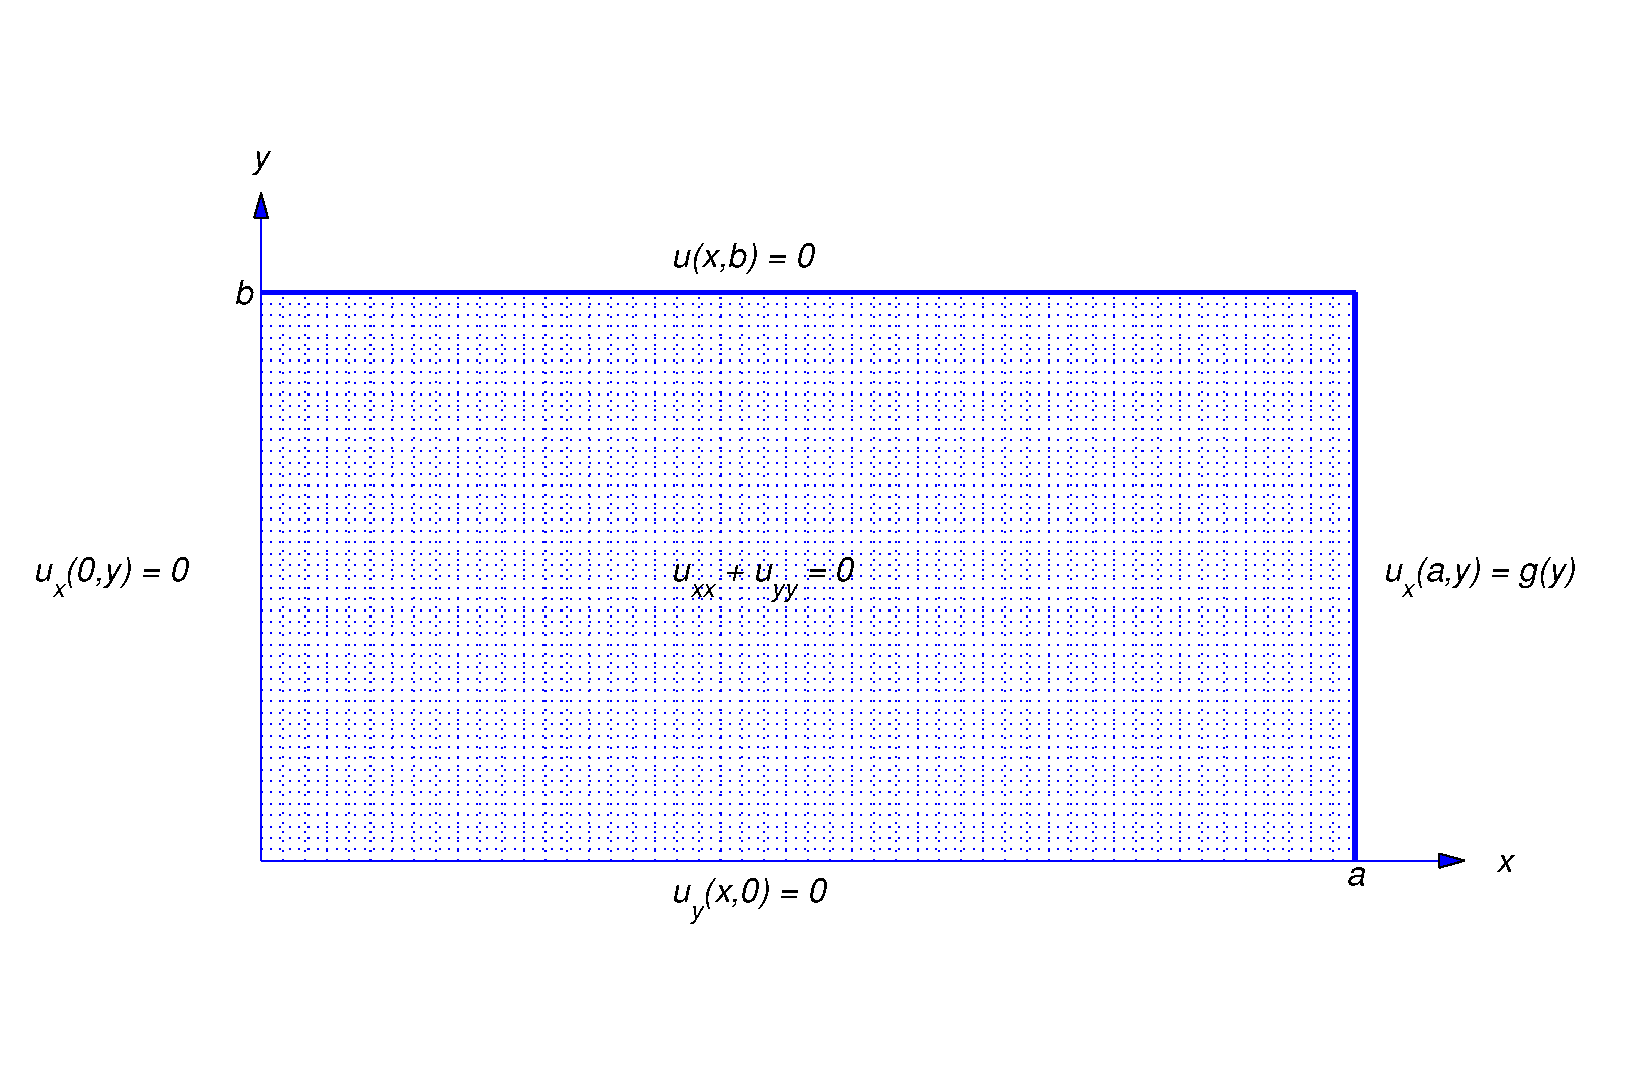
\includegraphics[bb=-78 148 689 643,width=5.67in,height=3.66in,keepaspectratio]{fig120311}
\caption{ The boundary value problem \eqref{eq:12.3.20}}
  \label{figure:12.3.11}
\end{figure}

\solution
The boundary conditions in \eqref{eq:12.3.20} require
 products $v(x,y)=X(x)Y(y)$ such that
$Y'(0)=Y(b)=X'(0)=0$; hence, we let $k=\lambda$ in
\eqref{eq:12.3.3}. Thus, $X$ and $Y$ must satisfy
\begin{equation} \label{eq:12.3.21}
X''-\lambda X=0,\quad \quad X'(0)=0
\end{equation}
and
\begin{equation} \label{eq:12.3.22}
Y''+\lambda Y=0,\quad Y'(0)=0,\quad Y(b)=0.
\end{equation}
 From Theorem~\ref{thmtype:11.1.4}, the eigenvalues of \eqref{eq:12.3.22}
are $\lambda_n=(2n-1)^2\pi^2/4b^2$, with
associated eigenfunctions
$$
Y_n=\cos{(2n-1)\pi y\over2b}, \quad n=1,2,3,\dots.
$$
Substituting $\lambda=(2n-1)^2\pi^2/4b^2$  into
\eqref{eq:12.3.21} yields
$$
X''-((2n-1)^2\pi^2/4b^2)X=0,\quad X'(0)=0,
$$
so we could take
\begin{equation} \label{eq:12.3.23}
X_n=\cosh{(2n-1)\pi x\over 2b}.
\end{equation}
However, because of the nonhomogeneous Neumann condition at $x=a$, it's
better to require that
$X_n'(a)=1$, which can be achieved by  dividing the right side
of
\eqref{eq:12.3.23} by the   value of its derivative  at $x=a$; thus,
$$
X_n=
{2b\cosh(2n-1)\pi x/2b\over(2n-1)\pi\sinh(2n-1)\pi a/2b}.
$$
Then
$$
v_n(x,y)=X_n(x)Y_n(y)=
{2b\cosh(2n-1)\pi x/2b\over(2n-1)\pi\sinh(2n-1)\pi a/2b}\cos{(2n-1)\pi
y\over2b},
$$
so
$$
{\partial v_n\over\partial x}(a,y)=\cos{(2n-1)\pi y\over2b}.
$$
Therefore
 $v_n$ satisfies \eqref{eq:12.3.20} with $g(y)=\cos(2n-1)\pi y/2b$. More
generally,
 if $\alpha_1$, \dots, $\alpha_m$ are arbitrary constants
then
$$
u_m(x,y)={2b\over\pi}\sum_{n=1}^m \alpha_n
{\cosh(2n-1)\pi x/2b\over(2n-1)\sinh(2n-1)\pi a/2b}\cos{(2n-1)\pi y\over 2b}
$$
satisfies \eqref{eq:12.3.20} with
$$
g(y)=\sum_{n=1}^\infty \alpha_n\cos{(2n-1)\pi
y\over2b}.
$$
Therefore, if $g$ is an arbitrary piecewise smooth function on
$[0,b]$,  we define the formal solution of \eqref{eq:12.3.20} to be
$$
u(x,y)={2b\over\pi}\sum_{n=1}^\infty \alpha_n
{\cosh(2n-1)\pi x/2b\over(2n-1)\sinh(2n-1)\pi a/2b}\cos{(2n-1)\pi y\over 2b},
$$
where
$$
C_M(y)=\sum_{n=1}^\infty \alpha_n\cos{(2n-1)\pi
y\over2b}
$$
 is the mixed Fourier cosine series of $g$ on $[0,b]$;
that is,
$$
\alpha_n={2\over b}\int_0^bg(y)\cos{(2n-1)\pi y\over2b}\,dy.
$$

\begin{example}\label{example:12.3.8}    \rm
Solve \eqref{eq:12.3.20} with $g(y)=y-b$.
\end{example}

\solution  From Example~\ref{example:11.3.3},
$$
C_M(y)=-{8b\over\pi^2}\sum_{n=1}^\infty{1\over(2n-1)^2}
\cos{(2n-1)\pi y\over2b}.
$$
Therefore
$$
u(x,y)=-{16b^2\over\pi^3}\sum_{n=1}^\infty{
\cosh(2n-1)\pi x/2b\over(2n-1)^3\sinh(2n-1)\pi a/2b}
\cos{(2n-1)\pi y\over2b}.
\eqno{\bbox}
$$

\boxit{Laplace's Equation for a Semi-Infinite Strip}

\noindent
We now seek solutions of Laplace's equation on
the semi-infinite strip
$$
S:\{0<x<a,\quad y>0\}
$$
(Figure~\ref{figure:12.3.12})
that satisfy homogeneous boundary conditions at $x=0$ and $x=a$, and
a nonhomogeneous  Dirichlet or Neumann condition at $y=0$. An
example of such a problem is
\begin{equation} \label{eq:12.3.24}
\begin{array}{c}
u_{xx}+u_{yy}=0,\quad 0<x<a,\quad  y>0,\\
u(x,0)=f(x),\quad 0\le x\le a,\\
u(0,y)=0,\quad u(a,y)=0,\quad y>0,
\end{array}
\end{equation}

   \begin{figure}[tbp]
  \centering\color{blue}
  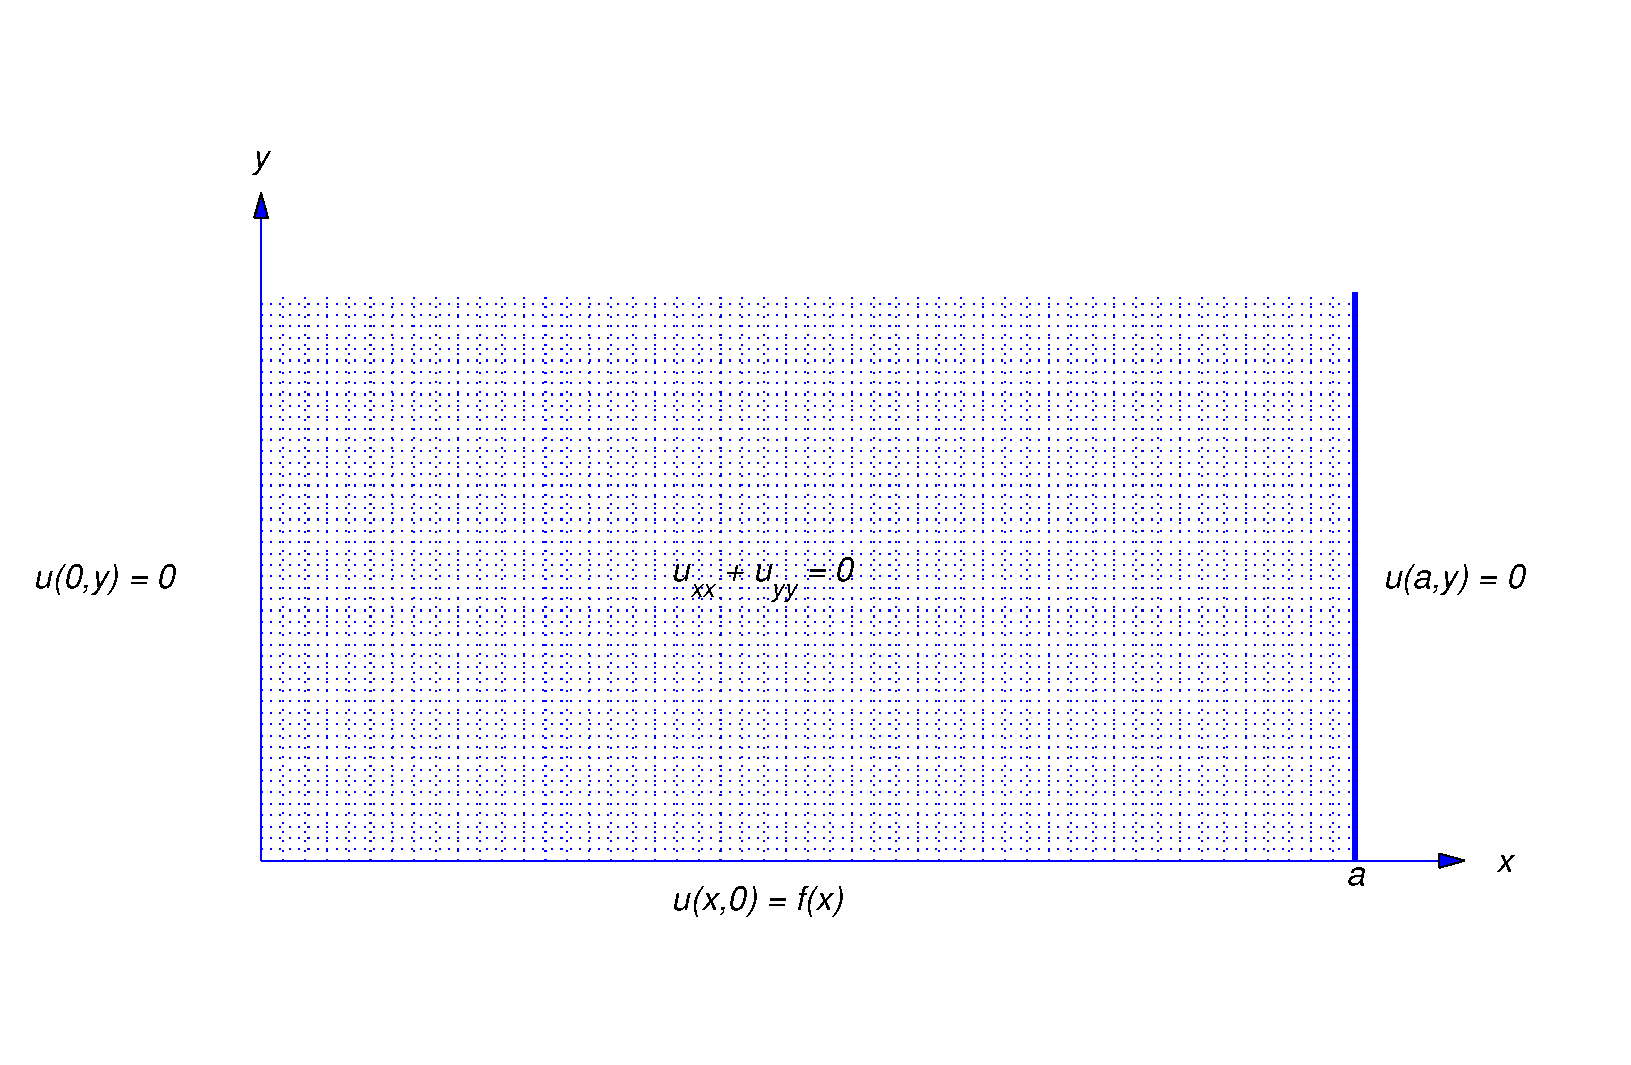
\includegraphics[bb=-78 148 689 643,width=5.67in,height=3.66in,keepaspectratio]{fig120312}
\caption{ A boundary value problem on a semi-infinite strip}
  \label{figure:12.3.12}
\end{figure}

The boundary conditions in this problem are not sufficient to
determine
$u$, for if $u_0=u_0(x,y)$ is a solution
and $K$ is a constant then
$$
u_1(x,y)=u_0(x,y)+K\sin{\pi x\over a}\sinh{\pi y\over a}.
$$
is also a solution. (Verify.) However, if we also require ---
on physical grounds --- that the solution remain bounded
for all $(x,y)$ in $S$
 then $K=0$ and this difficulty is eliminated.

\begin{example}\label{example:12.3.9} \rm
Define the bounded formal solution of
\eqref{eq:12.3.24}.
\end{example}

\solution Proceeding as in the solution of Example~\ref{example:12.3.1},
we find that the building block functions are of the form
$$
v_n(x,y)=Y_n(y)\sin{n\pi x\over a},
$$
where
$$
Y_n''-(n^2\pi^2/a^2)Y_n=0.
$$
Therefore
$$
Y_n=c_1e^{n\pi y/a}+c_2e^{-n\pi y/a}
$$
where $c_1$ and $c_2$ are constants.
Although the boundary conditions in \eqref{eq:12.3.24}  don't restrict
$c_1$, and $c_2$, we must set $c_1=0$ to ensure that $Y_n$ is bounded.
Letting $c_2=1$ yields
$$
v_n(x,y)=e^{-n\pi y/a}\sin{n\pi x\over a},
$$
and we define the bounded formal solution of \eqref{eq:12.3.24} to be
$$
u(x,y)=\sum_{n=1}^\infty b_ne^{-n\pi y/a}\sin{n\pi x\over a},
$$
where
$$
S(x)=\sum_{n=1}^\infty b_n\sin{n\pi x\over a}
$$
is the Fourier sine series of $f$ on $[0,a]$.
\bbox

See Exercises~\ref{exer:12.3.29}-\ref{exer:12.3.34}  for other boundary value
problems  on a semi-infinite strip.

\exercises
In Exercises~\ref{exer:12.3.1}-\ref{exer:12.3.16} apply the definition
developed in Example~1 to  solve the boundary
value problem. (Use Theorem~\ref{thmtype:11.3.5} where it
applies.)
 Where indicated by \Cex, graph the surface
$u=u(x,y)$, $0\le x\le a$, $0\le y\le b$.

\begin{exerciselist}

\item\label{exer:12.3.1}
$u_{xx}+u_{yy}=0,\quad 0<x<1,\quad  0<y<1,$\\
$u(x,0)=x(1-x),\quad u(x,1)=0,\quad 0\le x\le 1,$\\
$u(0,y)=0,\quad u(1,y)=0,\quad 0\le y\le 1$

\item\label{exer:12.3.2}
$u_{xx}+u_{yy}=0,\quad 0<x<2,\quad  0<y<3,$\\
$u(x,0)=x^2(2-x),\quad u(x,3)=0,\quad 0\le x\le 2,$\\
$u(0,y)=0,\quad u(2,y)=0,\quad 0\le y\le 3$

\item\label{exer:12.3.3}  \Cex
$u_{xx}+u_{yy}=0,\quad 0<x<2,\quad  0<y<2,$\\
$u(x,0)=
\left\{\begin{array}{cl}
x,& 0\le x\le 1,\\
2-x,&1\le x\le2,
\end{array}\right.
\quad u(x,2)=0,\quad 0\le x\le 2,$\\
$u(0,y)=0,\quad u(2,y)=0,\quad 0\le y\le 2$

\item\label{exer:12.3.4}
$u_{xx}+u_{yy}=0,\quad 0<x<\pi,\quad  0<y<1,$\\
$u(x,0)=x\sin x,\quad u(x,\pi)=0,\quad 0\le x\le \pi,$\\
$u(0,y)=0,\quad u(\pi,y)=0,\quad 0\le y\le 1$

\item\label{exer:12.3.5}
$u_{xx}+u_{yy}=0,\quad 0<x<3,\quad  0<y<2,$\\
$u(x,0)=0,\quad u_y(x,2)=x^2,\quad 0\le x\le 3,$\\
$u_x(0,y)=0,\quad u_x(3,y)=0,\quad 0\le y\le 2$

\item\label{exer:12.3.6}
$u_{xx}+u_{yy}=0,\quad 0<x<1,\quad  0<y<2,$\\
$u(x,0)=0,\quad u_y(x,2)=1-x,\quad 0\le x\le 1,$\\
$u_x(0,y)=0,\quad u_x(1,y)=0,\quad 0\le y\le 2$

\item\label{exer:12.3.7}
$u_{xx}+u_{yy}=0,\quad 0<x<2,\quad  0<y<2,$\\
$u(x,0)=0,\quad u_y(x,2)=x^2-4,\quad 0\le x\le 2,$\\
$u_x(0,y)=0,\quad u_x(2,y)=0,\quad 0\le y\le 2$

\item\label{exer:12.3.8}
$u_{xx}+u_{yy}=0,\quad 0<x<1,\quad  0<y<1,$\\
$u(x,0)=0,\quad u_y(x,1)=(x-1)^2,\quad 0\le x\le 1,$\\
$u_x(0,y)=0,\quad u_x(1,y)=0,\quad 0\le y\le 1$

\item\label{exer:12.3.9}   \Cex
$u_{xx}+u_{yy}=0,\quad 0<x<3,\quad  0<y<2,$\\
$u(x,0)=0,\quad u_y(x,2)=0,\quad 0\le x\le 3,$\\
$u(0,y)=y(4-y),\quad u_x(3,y)=0,\quad 0\le y\le 2$

\item\label{exer:12.3.10}
$u_{xx}+u_{yy}=0,\quad 0<x<2,\quad  0<y<1,$\\
$u(x,0)=0,\quad u_y(x,1)=0,\quad 0\le x\le 2,$\\
$u(0,y)=y^2(3-2y),\quad u_x(2,y)=0,\quad 0\le y\le 1$

\item\label{exer:12.3.11}
$u_{xx}+u_{yy}=0,\quad 0<x<2,\quad  0<y<2,$\\
$u(x,0)=0,\quad u_y(x,2)=0,\quad 0\le x\le 2,$\\
$u(0,y)=(y-2)^3+8,\quad u_x(2,y)=0,\quad 0\le y\le 2$

\item\label{exer:12.3.12}
$u_{xx}+u_{yy}=0,\quad 0<x<3,\quad  0<y<1,$\\
$u(x,0)=0,\quad u_y(x,1)=0,\quad 0\le x\le 3,$\\
$u(0,y)=y(2y^2-9y+12),\quad u_x(3,y)=0,\quad 0\le y\le 1$

\item\label{exer:12.3.13}  \Cex
$u_{xx}+u_{yy}=0,\quad 0<x<1,\quad  0<y<\pi,$\\
$u_y(x,0)=0,\quad u(x,\pi)=0,\quad 0\le x\le 1,$\\
$u_x(0,y)=0,\quad u_x(1,y)=\sin y,\quad 0\le y\le \pi$

\item\label{exer:12.3.14}
$u_{xx}+u_{yy}=0,\quad 0<x<2,\quad  0<y<3,$\\
$u_y(x,0)=0,\quad u(x,3)=0,\quad 0\le x\le 2,$\\
$u_x(0,y)=0,\quad u_x(2,y)=y(3-y),\quad 0\le y\le 3$

\item\label{exer:12.3.15}
$u_{xx}+u_{yy}=0,\quad 0<x<1,\quad  0<y<\pi,$\\
$u_y(x,0)=0,\quad u(x,\pi)=0,\quad 0\le x\le 1,$\\
$u_x(0,y)=0,\quad u_x(1,y)=\pi^2-y^2,\quad 0\le y\le \pi$

\item\label{exer:12.3.16}
$u_{xx}+u_{yy}=0,\quad 0<x<1,\quad  0<y<1,$\\
$u_y(x,0)=0,\quad u(x,1)=0,\quad 0\le x\le 1,$\\
$u_x(0,y)=0,\quad u_x(1,y)=1-y^3,\quad 0\le y\le 1$

\exercisetext{In
Exercises~\ref{exer:12.3.17}-\ref{exer:12.3.28} define the formal solution of
$$
u_{xx}+u_{yy}=0,\quad 0<x<a,\quad 0<y<b
$$
that satisfies the given boundary conditions for general $a$, $b$,
and $f$ or $g$.
Then solve the boundary value problem for the specified  $a$,
$b$, and  $f$ or $g$.
 (Use Theorem~\ref{thmtype:11.3.5} where it applies.)
Where indicated by \Cex, graph the surface
$u=u(x,y)$, $0\le x\le a$, $0\le y\le b$.}

\item\label{exer:12.3.17}  \Cex
$u(x,0)=0,\quad u(x,b)=f(x),\quad 0<x<a,\\
u(0,y)=0,\quad u(a,y)=0,\quad 0<y<b$  \\
$a=3$,\quad $b=2$,\quad $f(x)=x(3-x)$

\item\label{exer:12.3.18}
$u(x,0)=f(x),\quad u(x,b)=0,\quad 0<x<a,\\
u_x(0,y)=0,\quad u_x(a,y)=0,\quad 0<y<b$  \\
$a=2$,\quad $b=1$,\quad $f(x)=x^2(x-2)^2$

\item\label{exer:12.3.19}
$u(x,0)=f(x),\quad u(x,b)=0,\quad 0<x<a,\\
u_x(0,y)=0,\quad u(a,y)=0,\quad 0<y<b$  \\
$a=1$,\quad $b=2$,\quad $f(x)=3x^3-4x^2+1$

\item\label{exer:12.3.20}
$u(x,0)=f(x),\quad u(x,b)=0,\quad 0<x<a,\\
u(0,y)=0,\quad u_x(a,y)=0,\quad 0<y<b$  \\
$a=3$,\quad $b=2$,\quad $f(x)=x(6-x)$

\item\label{exer:12.3.21}
$u(x,0)=f(x),\quad u_y(x,b)=0,\quad 0<x<a,\\
u(0,y)=0,\quad u(a,y)=0,\quad 0<y<b$  \\
$a=\pi$,\quad $b=2$,\quad $f(x)=x(\pi^2-x^2)$

\item\label{exer:12.3.22}
$u_y(x,0)=0,\quad u(x,b)=f(x),\quad 0<x<a,\\
u_x(0,y)=0,\quad u_x(a,y)=0,\quad 0<y<b$  \\
$a=\pi$,\quad $b=1$,\quad $f(x)=x^2(x-\pi)^2$

\item\label{exer:12.3.23} \Cex
$u_y(x,0)=f(x),\quad u(x,b)=0,\quad 0<x<a,\\
u(0,y)=0,\quad u(a,y)=0,\quad 0<y<b$  \\
$a=\pi$,\quad  $b=1$,\quad
$f(x)=
\left\{\begin{array}{cl}
x,&0\le x\le{\pi\over2},\\\pi-x,&{\pi\over2}\le x\le \pi
\end{array}\right.$

\item\label{exer:12.3.24}
$u(x,0)=0,\quad u(x,b)=0,\quad 0<x<a,\\
u_x(0,y)=0,\quad u(a,y)=g(y),\quad 0<y<b$  \\
$a=1$,\quad $b=1$,\quad $g(y)=y(y^3-2y^2+1)$

\item\label{exer:12.3.25} \Cex
$u_y(x,0)=0,\quad u(x,b)=0,\quad 0<x<a,\\
u_x(0,y)=0,\quad u(a,y)=g(y),\quad 0<y<b$  \\
$a=2$,\quad $b=2$,\quad $g(y)=4-y^2$

\item\label{exer:12.3.26}
$u(x,0)=0,\quad u(x,b)=0,\quad 0<x<a,\\
u_x(0,y)=0,\quad u_x(a,y)=g(y),\quad 0<y<b$  \\
$a=1$, $b=4$,
$g(y)=
\left\{\begin{array}{cl}
y,&0\le y\le2,\\4-y,&2\le y\le 4
\end{array}\right.$

\item\label{exer:12.3.27}
$u(x,0)=0,\quad u_y(x,b)=0,\quad 0<x<a,\\
u_x(0,y)=g(y),\quad u_x(a,y)=0,\quad 0<y<b$  \\
$a=1$,\quad  $b=\pi$,\quad $g(y)=y^2(3\pi-2y)$

\item\label{exer:12.3.28}
$u_y(x,0)=0,\quad u_y(x,b)=0,\quad 0<x<a,\\
u_x(0,y)=g(y),\quad u(a,y)=0,\quad 0<y<b$  \\
$a=2$,\quad $b=\pi$,\quad $g(y)=y$

\exercisetext{In
Exercises~\ref{exer:12.3.29}-\ref{exer:12.3.34} define the bounded formal
solution of
$$
u_{xx}+u_{yy}=0,\quad 0<x<a,\quad y>0
$$
that satisfies the given boundary conditions for general $a$ and $f$.
Then solve the boundary value problem for the specified  $a$
and  $f$.}

\item\label{exer:12.3.29}
$u(x,0)=f(x),\quad 0<x<a$,\quad\\
$u_x(0,y)=0,\quad u_x(a,y)=0,\quad y>0$  \\
$a=\pi$   $f(x)=x^2(3\pi-2x)$

\item\label{exer:12.3.30}
$u(x,0)=f(x),\quad 0<x<a$,\\
$u_x(0,y)=0,\quad u(a,y)=0,\quad y>0$  \\
$a=3$,\quad $f(x)=9-x^2$

\item\label{exer:12.3.31}
$u(x,0)=f(x),\quad 0<x<a$,\quad\\
$u(0,y)=0,\quad u_x(a,y)=0,\quad y>0$  \\
$a=\pi$,\quad $f(x)=x(2\pi-x)$

\item\label{exer:12.3.32}
$u_y(x,0)=f(x),\quad 0<x<a$,\\
$u(0,y)=0,\quad u(a,y)=0,\quad y>0$  \\
$a=\pi$,\quad $f(x)=x^2(\pi-x)$

\item\label{exer:12.3.33}
$u_y(x,0)=f(x),\quad 0<x<a$, \\
$u_x(0,y)=0,\quad u(a,y)=0,\quad y>0$  \\
$a=7$,\quad $f(x)=x(7-x)$

\item\label{exer:12.3.34}
$u_y(x,0)=f(x),\quad 0<x<a$,\\
$u(0,y)=0,\quad u_x(a,y)=0,\quad y>0$  \\
$a=5$,\quad $f(x)=x(5-x)$

\item\label{exer:12.3.35}
Define the formal solution of the Dirichlet problem
$$
\begin{array}{c}
u_{xx}+u_{yy}=0,\quad 0<x<a,\quad  0<y<b,\\
u(x,0)=f_0(x),\quad u(x,b)=f_1(x),\quad 0\le x\le a,\\
u(0,y)=g_0(y),\quad u(a,y)=g_1(y),\quad 0\le y\le b
\end{array}
$$

\item\label{exer:12.3.36}
Show that the  Neumann Problem
$$
\begin{array}{c}
u_{xx}+u_{yy}=0,\quad 0<x<a,\quad  0<y<b,\\
u_y(x,0)=f_0(x),\quad u_y(x,b)=f_1(x),\quad 0\le x\le a,\\
u_x(0,y)=g_0(y),\quad u_x(a,y)=g_1(y),\quad 0\le y\le b
\end{array}
$$
has no solution unless
$$
\int_0^af_0(x)\,dx=
\int_0^af_1(x)\,dx=
\int_0^bg_0(y)\,dy=
\int_0^bg_1(y)\,dy=0.
$$
In this case it has infinitely many formal solutions.
Find  them.

\item\label{exer:12.3.37}
In this exercise
take it as given that the infinite series $\sum_{n=1}^\infty
n^pe^{-qn}$ converges for all $p$ if $q>0$, and, where appropriate,
use the comparison test for absolute convergence of an infinite
series.

Let
$$
u(x,y)=\sum_{n=1}^\infty \alpha_n
{\sinh n\pi(b-y)/a\over\sinh n\pi b/a}
\sin{n\pi x\over a},
$$
where
$$
\alpha_n={2\over a}\int_0^a f(x)\sin{n\pi x\over a}\,dx
$$
and $f$ is piecewise smooth on $[0,a]$.

\begin{alist}
\item % (a)
Verify the approximations
$$
{\sinh n\pi(b-y)/a\over\sinh n\pi b/a}\approx e^{-n\pi y/a},\quad y<b,
\eqno{\rm(A)}
$$
and
$$
{\cosh n\pi(b-y)/a\over\sinh n\pi b/a}\approx e^{-n\pi y/a},\quad y<b
\eqno{\rm(B)}
$$
for large $n$.
\item % (b)
Use (A) to show that
 $u$ is defined for $(x,y)$ such that $0<y<b$.
\item % (c)
For fixed $y$ in $(0,b)$,
use (A) and Theorem~\ref{thmtype:12.1.2} with $z=x$
 to show that
$$
u_x(x,y)={\pi\over a}\sum_{n=1}^\infty n\alpha_n
{\sinh n\pi(b-y)/a\over\sinh n\pi b/a}
\cos{n\pi x\over a},\quad -\infty<x< \infty.
$$
\item % (d)
Starting from the result of \part{b},
use (A) and Theorem~\ref{thmtype:12.1.2} with $z=x$
 to show that, for a fixed $y$ in $(0,b)$,
$$
u_{xx}(x,y)=-{\pi^2\over a^2}\sum_{n=1}^\infty n^2\alpha_n
{\sinh n\pi(b-y)/a\over\sinh n\pi b/a}
\sin{n\pi x\over a},\quad -\infty<x< \infty.
$$
\item % (e)
For fixed but arbitrary $x$,
use (B) and Theorem~\ref{thmtype:12.1.2} with $z=y$
 to show that
$$
u_y(x,y)=-{\pi\over a}\sum_{n=1}^\infty n\alpha_n
{\cosh n\pi(b-y)/a\over\sinh n\pi b/a}
\sin{n\pi x\over a}
$$
if $0<y_0<y<b$, where $y_0$ is an  arbitrary
number in $(0,b)$.
 Then argue that since $y_0$ can be chosen arbitrarily small,
the conclusion holds for all $y$ in $(0,b)$.
\item % (f)
Starting from the result of \part{e}, use (A) and
Theorem~\ref{thmtype:12.1.2} to show that
$$
u_{yy}(x,y)={\pi^2\over a^2}\sum_{n=1}^\infty n^2\alpha_n
{\sinh n\pi(b-y)/a\over\sinh n\pi b/a}
\sin{n\pi x\over a},\quad 0<y<b.
$$
\item % (g)
Conclude that $u$ satisfies Laplace's equation for all $(x,y)$
such that $0<y<b$.
\end{alist}

By repeatedly applying the arguments in \part{c}--\part{f},
it can be shown that $u$ can be differentiated term by term any
number of times with respect to $x$ and/or $y$ if $0<y<b$.

\end{exerciselist}


\section{Laplace's Equation in Polar Coordinates}

\noindent
In Section~12.3 we solved boundary value
problems for Laplace's equation over a rectangle with sides parallel
to the $x,y$-axes. Now we'll consider boundary value problems for
Laplace's equation over regions with boundaries best described in
terms of polar coordinates. In this case it's appropriate to regard
$u$ as function of $(r,\theta)$ and write Laplace's equation in polar
form as
\begin{equation} \label{eq:12.4.1}
u_{rr}+\frac{1}{r}u_r+\frac{1}{r^2}u_{\theta\theta}=0,
\end{equation}
where
$$
r=\sqrt{x^2+y^2}\mbox{\quad and \quad}
\theta=\cos^{-1}\frac{x}{r}=\sin^{-1}\frac{x}{r}.
$$

We begin with the case where the region
 is a circular disk with radius $\rho$, centered at the origin;   that
is, we want to define a formal solution of the boundary value problem
\begin{equation} \label{eq:12.4.2}
\begin{array}{c}
\dst u_{rr}+\frac{1}{r}u_r+\frac{1}{r^2}u_{\theta\theta}=0,\quad
0<r<\rho,\quad -\pi\le\theta<\pi,\\[2\jot]
u(\rho,\theta)=f(\theta),\quad -\pi\le\theta<\pi
\end{array}
\end{equation}
(Figure~\ref{figure:12.4.1}).
Note that \eqref{eq:12.4.2} imposes no restriction on $u(r,\theta)$
when $r=0$. We'll address this question at
the appropriate time.

\begin{figure}[H]
  \centering\color{blue}
  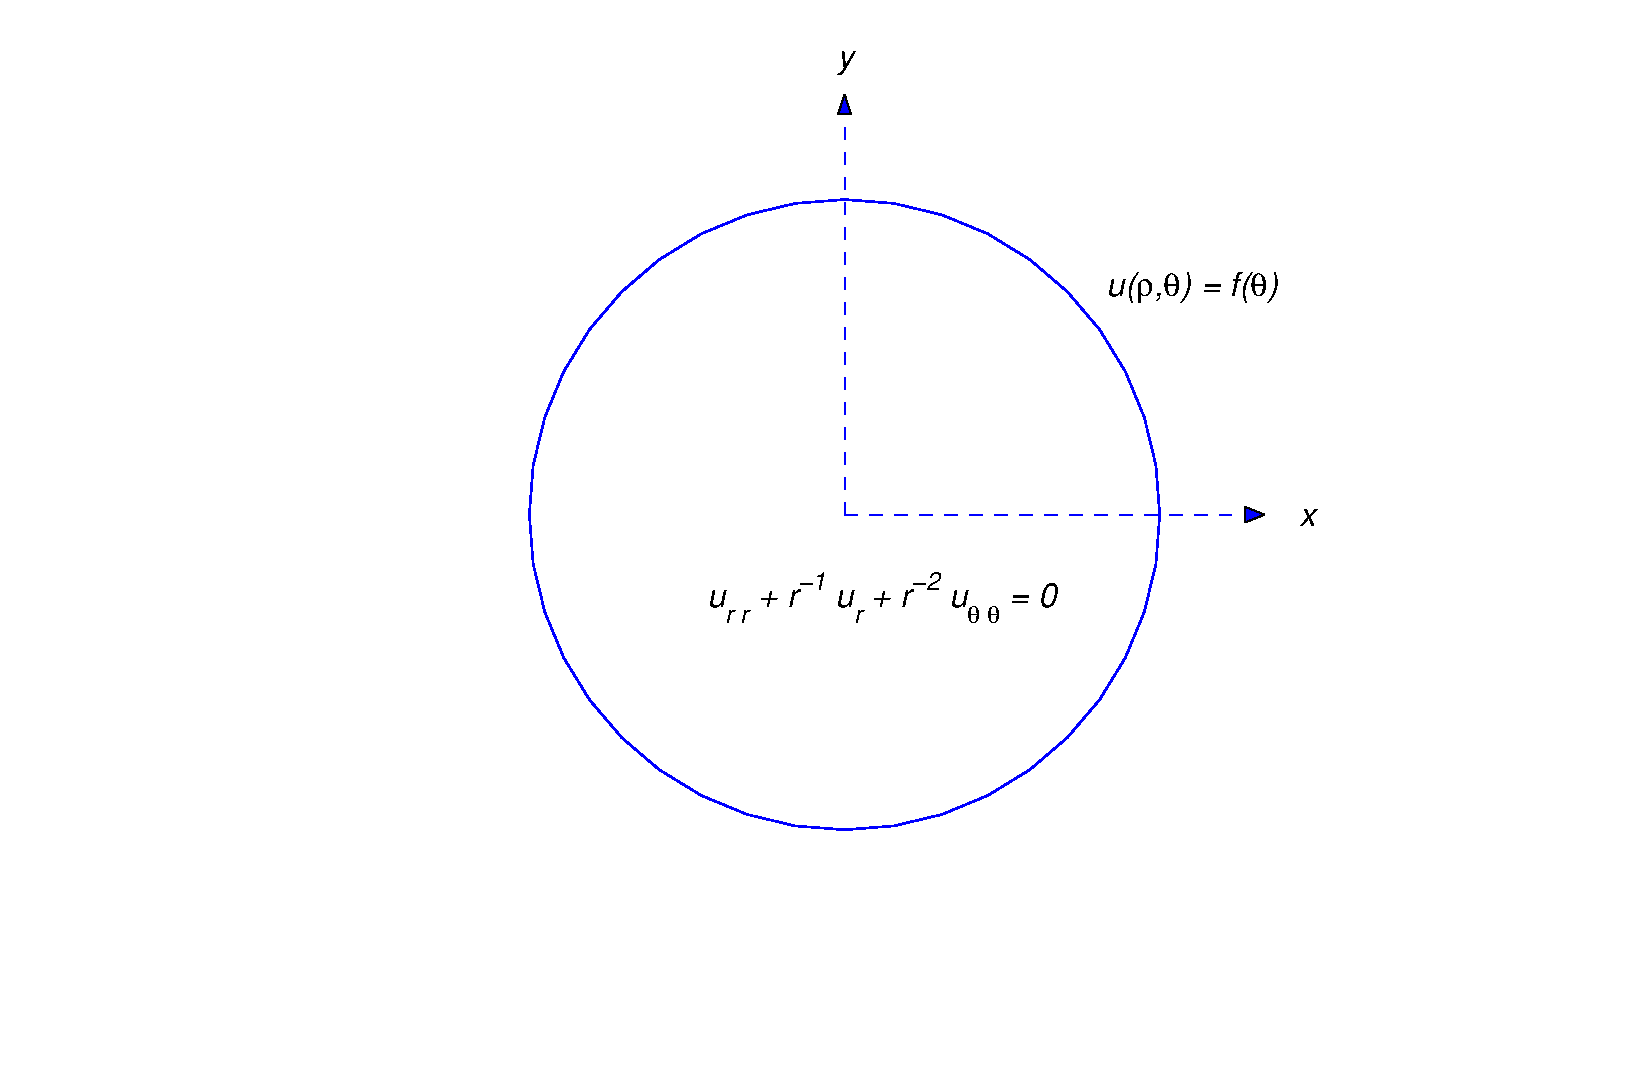
\includegraphics[bb=-78 148 689 643,width=5.67in,height=3.66in,keepaspectratio]{fig120401}
\caption{ The boundary value problem \eqref{eq:12.4.2}}
  \label{figure:12.4.1}
\end{figure}

We first look for products
$v(r,\theta)=R(r)\Theta(\theta)$ that satisfy \eqref{eq:12.4.1}. For
this function,
$$
v_{rr}+\frac{1}{r}v_r+\frac{1}{r^2}v_{\theta\theta}=
R''\Theta+\frac{1}{r}R'\Theta
+\frac{1}{r^2}R\Theta''=0
$$
for all $(r,\theta)$ with $r\ne0$ if
$$
\frac{r^2R''+rR'}{R}=-\frac{\Theta''}{\Theta}=\lambda,
$$
where $\lambda$ is a separation constant. (Verify.)
This equation is equivalent to
$$
\Theta''+\lambda\Theta=0
$$
and
\begin{equation} \label{eq:12.4.3}
r^2R''+rR'-\lambda R=0.
\end{equation}
Since $(r,\pi)$ and $(r,-\pi)$ are the polar coordinates
of the same point, we impose periodic boundary conditions
on $\Theta$; that is,
\begin{equation} \label{eq:12.4.4}
\Theta''+\lambda\Theta=0,\quad \Theta(-\pi)=\Theta(\pi),
\quad \Theta'(-\pi)=\Theta'(\pi).
\end{equation}
Since we don't want  $R\Theta$ to be identically zero,
$\lambda$ must be an eigenvalue of \eqref{eq:12.4.4} and $\Theta$
must be an associated eigenfunction. From Theorem~\ref{thmtype:11.1.6},
the eigenvalues of \eqref{eq:12.4.4} are $\lambda_0=0$ with
associated eigenfunctions $\Theta_0=1$ and, for $n=1,2,3,\dots,$
$\lambda_n=n^2$,
with associated eigenfunction $\cos n\theta$ and $\sin n\theta$
therefore,
$$
 \Theta_n=\alpha_n\cos n\theta+\beta_n\sin n\theta
$$
where $\alpha_n$ and $\beta_n$ are constants.

Substituting $\lambda=0$ into \eqref{eq:12.4.3} yields the
$$
r^2R''+rR'=0,
$$
so
$$
\frac{R_0''}{R_0'}=-\frac{1}{r},
$$
$$
R_0'=\frac{c_1}{r},
$$
and
\begin{equation} \label{eq:12.4.5}
R_0=c_2+c_1\ln r.
\end{equation}
If $c_1\ne0$ then
$$
\lim_{r\to0+}|R_0(r)|=\infty,
$$
which doesn't make sense if we interpret
$u_0(r,\theta)=R_0(r)\Theta_0(\theta)=R_0(r)$ as the steady state
temperature distribution in a disk whose boundary is maintained
at the constant temperature $R_0(\rho)$.
Therefore we now require
$R_0$ to be bounded as $r\to0+$.  This implies that $c_1=0$, and
we  take $c_2=1$.
Thus, $R_0=1$ and $v_0(r,\theta)=R_0(r)\Theta_0(\theta)=1$.
Note that $v_0$ satisfies \eqref{eq:12.4.2} with
$f(\theta)=1$.

Substituting $\lambda=n^2$ into \eqref{eq:12.4.3} yields
the Euler equation
\begin{equation} \label{eq:12.4.6}
r^2R_n''+rR_n'-n^2 R_n=0
\end{equation}
for $R_n$.
The indicial polynomial of this equation is
$$
s(s-1)+s-n^2=(s-n)(s+n),
$$
so the general solution of \eqref{eq:12.4.6} is
\begin{equation} \label{eq:12.4.7}
R_n=c_1r^n+c_2r^{-n},
\end{equation}
by Theorem~\ref{thmtype:7.4.3}. Consistent with our previous assumption on
$R_0$, we now require  $R_n$  to be bounded as $r\to0+$.
This implies that  $c_2=0$, and we   choose
$c_1=\rho^{-n}$.
Then
$R_n(r)=r^n/\rho^n$, so
$$
v_n(r,\theta)=R_n(r)\Theta_n(\theta)=\frac{r^n}{\rho^n}(\alpha_n\cos
n\theta+\sin n\theta).
$$
Now  $v_n$ satisfies \eqref{eq:12.4.2} with
$$
f(\theta)=\alpha_n\cos n\theta+\beta_n\sin n\theta.
$$
More generally, if $\alpha_0$, $\alpha_1$,\dots, $\alpha_m$ and
$\beta_1$,
$\beta_2$,
\dots, $\beta_m$ are arbitrary constants then
$$
u_m(r,\theta)=\alpha_0+\sum_{n=1}^m\frac{r^n}{\rho^n}(\alpha_n\cos
n\theta+\beta_n\sin n\theta)
$$
satisfies \eqref{eq:12.4.2} with
$$
f(\theta)
=\alpha_0+\sum_{n=1}^m(\alpha_n\cos
n\theta+\beta_n\sin n\theta).
$$
This motivates the next definition.

\begin{definition}\color{blue} \label{thmtype:12.4.1} \rm
The bounded formal solution of the boundary value problem
\eqref{eq:12.4.2} is
\begin{equation} \label{eq:12.4.8}
u(r,\theta)=\alpha_0+\sum_{n=1}^\infty\frac{r^n}{\rho^n}(\alpha_n\cos
n\theta+\beta_n\sin n\theta),
\end{equation}
where
$$
F(\theta)
=\alpha_0+\sum_{n=1}^\infty(\alpha_n\cos
n\theta+\beta_n\sin n\theta)
$$
is the Fourier series of  $f$ on $[-\pi,\pi]$; that is,
$$
\alpha_0=\frac{1}{2\pi}\int_{-\pi}^\pi f(\theta)\,d\theta,
$$
and
$$
\alpha_n=\frac{1}{\pi}\int_{-\pi}^\pi f(\theta)\cos n\theta\,d\theta
\text{\quad and \quad}
\beta_n=\frac{1}{\pi}\int_{-\pi}^\pi f(\theta)\sin
n\theta\,d\theta,
\quad n=1,2,3,\dots.
$$
\end{definition}

Since $\sum_{n=0}^\infty n^k(r/\rho)^n$  converges for every
$k$ if $0< r<\rho$, Theorem~\ref{thmtype:12.1.2} can be used to show that if
$0< r<\rho$ then
 \eqref{eq:12.4.8} can be differentiated term by term
any number of times with respect to both $r$ and $\theta$.
Since the  terms in \eqref{eq:12.4.8} satisfy Laplace's
equation if $r>0$,  \eqref{eq:12.4.8} satisfies
Laplace's equation if $0<r<\rho$. Therefore, since
$u(\rho,\theta)=F(\theta)$,
$u$ is an actual solution of \eqref{eq:12.4.2} if and only if
$$
F(\theta)=f(\theta),\quad -\pi\le\theta<\pi.
$$
From Theorem~\ref{thmtype:11.2.4}, this is true if $f$ is continuous and piecewise
smooth on $[-\pi,\pi]$ and $f(-\pi)=f(\pi)$.

\begin{example}\label{example:12.4.1} \rm
Find the bounded formal solution of \eqref{eq:12.4.2} with
$f(\theta)=\theta(\pi^2-\theta^2)$.
\end{example}

\solution From  Example~\ref{example:11.2.6},
$$
\theta(\pi^2-\theta^2)=12\sum_{n=1}^\infty\frac{(-1)^n}{n^3}\sin
n\theta,\quad -\pi\le\theta\le\pi,
$$
so
$$
u(r,\theta)=12\sum_{n=1}^\infty\frac{r^n}{\rho^n}\frac{(-1)^n}{n^3}\sin
n\theta,\quad
0\le r\le \rho,\quad -\pi\le\theta\le\pi.
$$

\begin{example}\label{example:12.4.2} \rm
Define the formal solution of
\begin{equation} \label{eq:12.4.9}
\begin{array}{c}
\dst u_{rr}+\frac{1}{r}u_r+\frac{1}{r^2}u_{\theta\theta}=0,\quad
\rho_0<r<\rho,\quad -\pi\le\theta<\pi,\\[2\jot]
u(\rho_0,\theta)=0,\quad  u(\rho,\theta)=f(\theta),\quad
-\pi\le\theta<\pi,
\end{array}
\end{equation}
where $0<\rho_0<\rho$ (Figure~\ref{figure:12.4.2}).
\end{example}

 \begin{figure}[H]
  \centering\color{blue}
  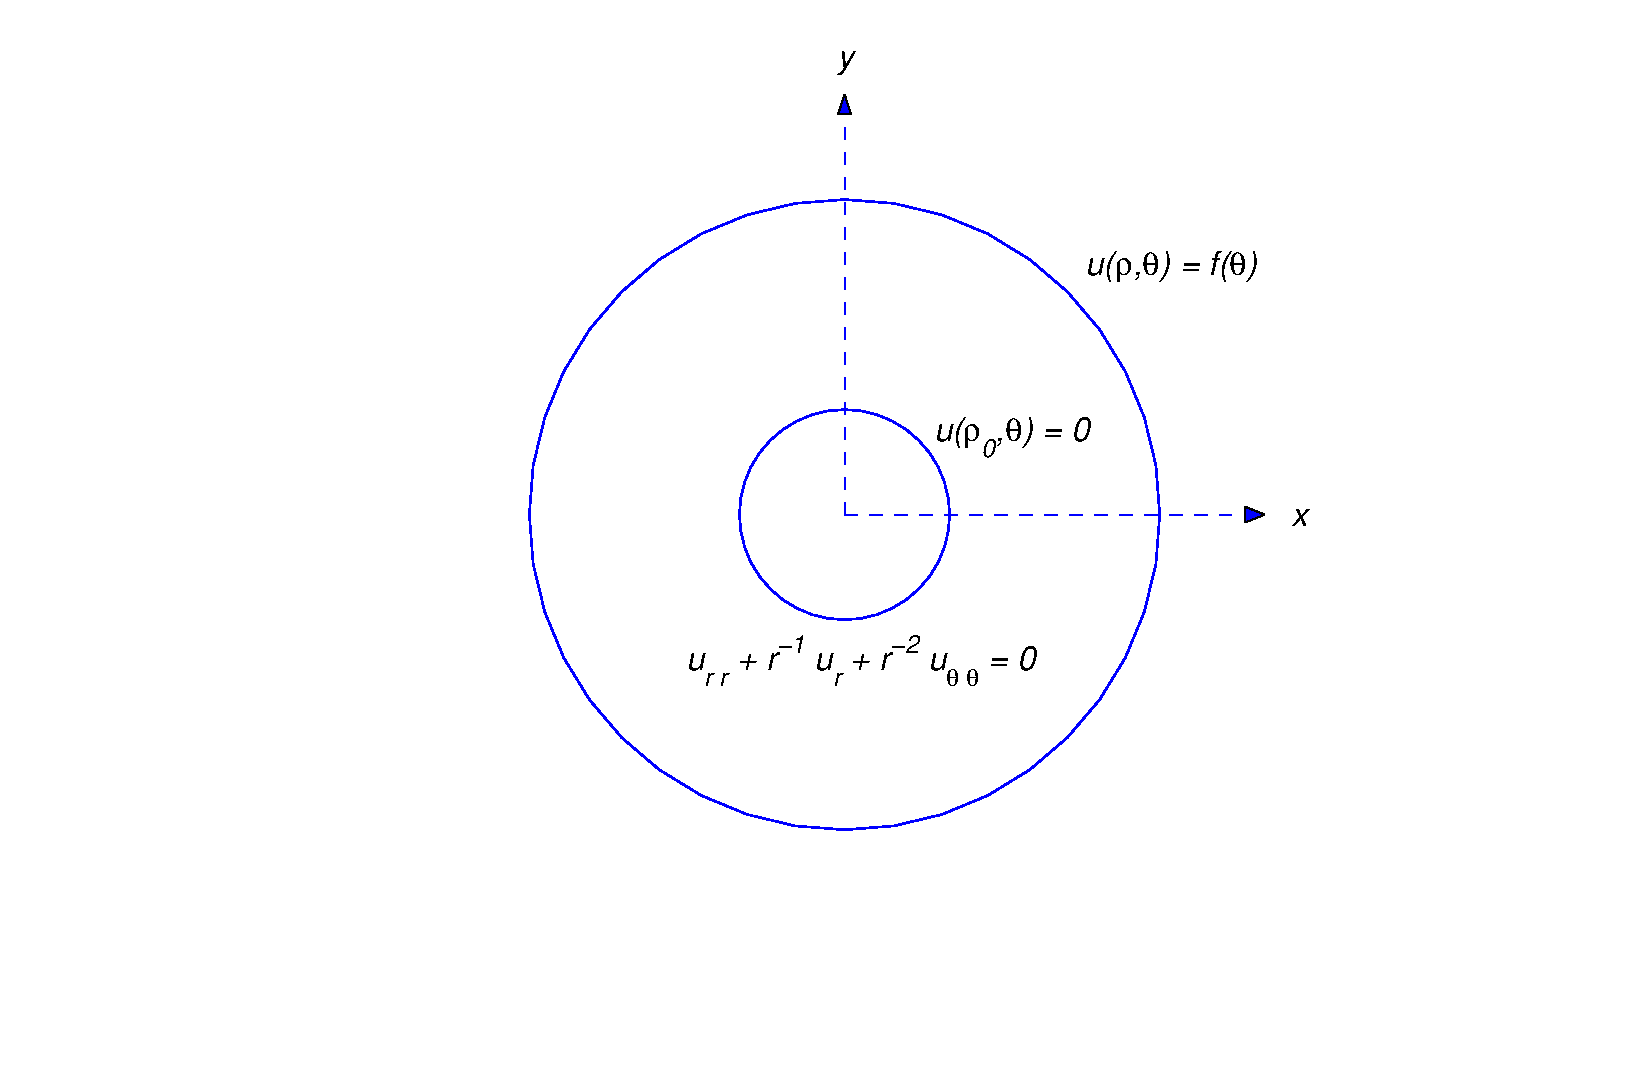
\includegraphics[bb=-78 148 689 643,width=5.67in,height=3.66in,keepaspectratio]{fig120402}
\caption{ The boundary value problem \eqref{eq:12.4.9}}
  \label{figure:12.4.2}
\end{figure}

\solution
We use separation of variables exactly as before, except that
now we choose the constants in \eqref{eq:12.4.5} and \eqref{eq:12.4.7}
so that $R_n(\rho_0)=0$ for $n=0$, $1$, $2$,\dots. In view of the
nonhomogeneous Dirichlet
condition on the boundary $r=\rho$, it's also convenient to require
that
$R_n(\rho)=1$ for $n=0$, $1$, $2$,\dots. We leave it to you to verify
that
$$
R_0(r)=\frac{\ln r/\rho_0}{\ln\rho/\rho_0}
\mbox{\quad and \quad}
R_n=\frac{\rho_0^{-n}r^n-\rho_0^nr^{-n}}
{\rho_0^{-n}\rho^n-\rho_0^n\rho^{-n}},\quad n=1,2,3,\dots
$$
satisfy these requirements. Therefore
$$
v_0(\rho,\theta)=\frac{\ln r/\rho_0}{\ln\rho/\rho_0}
$$
and
$$
v_n(r,\theta)=\frac{\rho_0^{-n}r^n-\rho_0^nr^{-n}}
{\rho_0^{-n}\rho^n-\rho_0^n\rho^{-n}}(\alpha_n\cos n\theta+\beta_n\sin
n\theta),
\quad n=1,2,3,\dots,
$$
where $\alpha_n$ and $\beta_n$ are arbitrary constants.

If $\alpha_0$, $\alpha_1$,\dots, $\alpha_m$ and
$\beta_1$,
$\beta_2$,
\dots, $\beta_m$ are arbitrary constants then
$$
u_m(r,\theta)=\alpha_0\frac{\ln r/\rho_0}{\ln\rho/\rho_0}+
\sum_{n=1}^m
\frac{\rho_0^{-n}r^n-\rho_0^nr^{-n}}
{\rho_0^{-n}\rho^n-\rho_0^n\rho^{-n}}
(\alpha_n\cos
n\theta+\beta_n\sin n\theta)
$$
satisfies \eqref{eq:12.4.9}, with
$$
f(\theta)
=\alpha_0+\sum_{n=1}^m(\alpha_n\cos
n\theta+\beta_n\sin n\theta).
$$
This motivates us to define the formal solution of \eqref{eq:12.4.9}
for general $f$ to be
$$
u(r,\theta)=\alpha_0\frac{\ln r/\rho_0}{\ln\rho/\rho_0}+
\sum_{n=1}^\infty
\frac{\rho_0^{-n}r^n-\rho_0^nr^{-n}}
{\rho_0^{-n}\rho^n-\rho_0^n\rho^{-n}}
(\alpha_n\cos
n\theta+\beta_n\sin n\theta),
$$
where
$$
F(\theta)
=\alpha_0+\sum_{n=1}^\infty(\alpha_n\cos
n\theta+\beta_n\sin n\theta)
$$
is the Fourier series of  $f$ on $[-\pi,\pi]$.

\begin{example}\label{example:12.4.3} \rm
Define the bounded formal solution of
\begin{equation} \label{eq:12.4.10}
\begin{array}{c}
\dst u_{rr}+\frac{1}{r}u_r+\frac{1}{r^2}u_{\theta\theta}=0,\quad
0<r<\rho,\quad 0<\theta<\gamma,\\[2\jot]
 u(\rho,\theta)=f(\theta),\quad 0\le\theta\le\gamma,\\[2\jot]
u(r,0)=0,\quad u(r,\gamma)=0,\quad 0<r<\rho,
\end{array}
\end{equation}
where $0<\gamma<2\pi$ (Figure~\ref{figure:12.4.3}).
\end{example}

\begin{figure}[tbp]
  \centering\color{blue}
  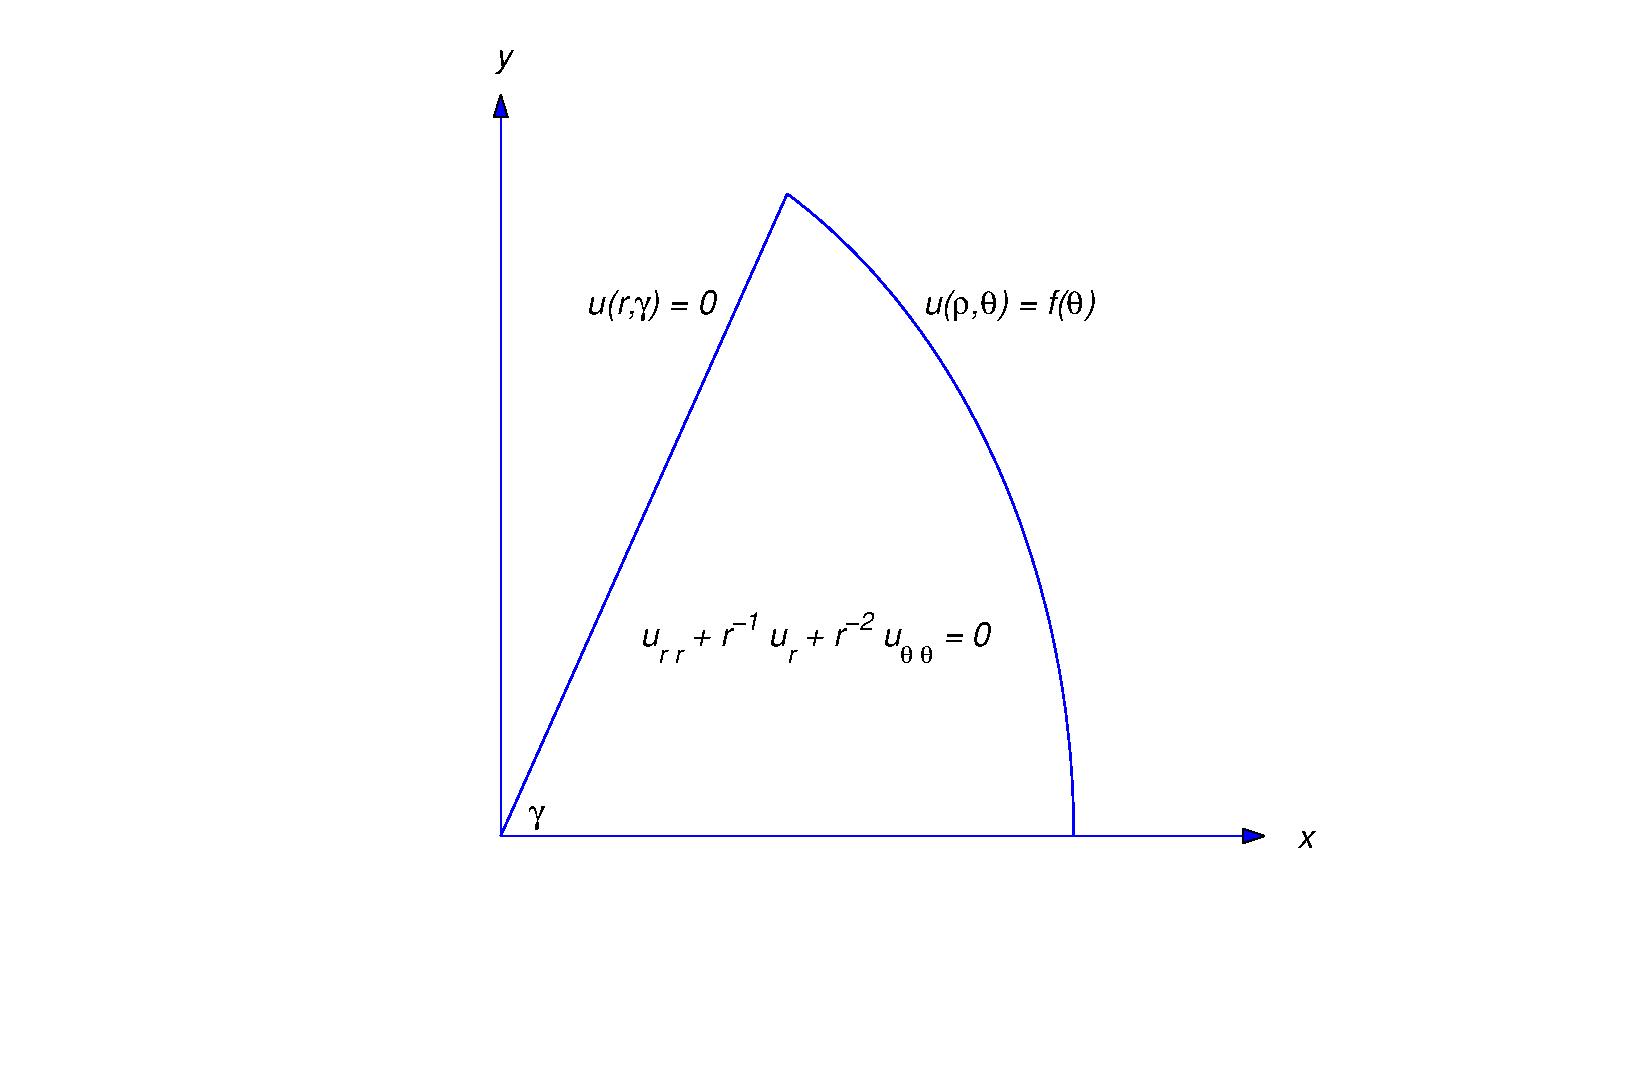
\includegraphics[bb=-78 148 689 643,width=5.67in,height=3.66in,keepaspectratio]{fig120403}
\caption{ The boundary value problem \eqref{eq:12.4.10}}
  \label{figure:12.4.3}
\end{figure}

\solution
Now $v(r,\theta)=R(r)\Theta(\theta)$, where
\begin{equation} \label{eq:12.4.11}
r^2R''+rR'-\lambda R=0
\end{equation}
and
\begin{equation} \label{eq:12.4.12}
\Theta''+\lambda\Theta=0,\quad \Theta(0)=0,\quad \Theta(\gamma)=0.
\end{equation}
From Theorem~\ref{thmtype:11.1.2},
the eigenvalues of \eqref{eq:12.4.12}  are
$\lambda_n=n^2\pi^2/\gamma^2$,
with associated eigenfunction $\Theta_n=\sin n\pi\theta/\gamma$,
$n=1$,  $2$, $3$,\dots.
Substituting $\lambda=n^2\pi^2/\gamma^2$ into \eqref{eq:12.4.11} yields
the Euler equation
$$
r^2R''+rR_n'-\frac{n^2\pi^2}{\gamma^2} R=0.
$$
The indicial polynomial of this equation is
$$
s(s-1)+s-\frac{n^2\pi^2}{\gamma^2}=\left(s-\frac{n\pi}{\gamma}\right)
\left(s+\frac{n\pi}{\gamma}\right),
$$
so
$$
R_n=c_1r^{n\pi/\gamma}+c_2r^{-n\pi/\gamma},
$$
by Theorem~\ref{thmtype:7.4.3}.
To obtain a solution that remains bounded as
$r\to0+$ we let $c_2=0$. Because of the Dirichlet condition at
$r=\rho$, it's convenient to have $r(\rho)=1$;   therefore we take
$c_1=\rho^{-n\pi/\gamma}$, so
$$
R_n(r)=\frac{r^{n\pi/\gamma}}{\rho^{n\pi/\gamma}}.
$$
Now
$$
v_n(r,\theta)=R_n(r)\Theta_n(\theta)=\frac{r^{n\pi/\gamma}}
{\rho^{n\pi/\gamma}}\sin\frac{n\pi\theta}{\gamma}
$$
 satisfies \eqref{eq:12.4.10} with
$$
f(\theta)=\sin\frac{n\pi\theta}{\gamma}.
$$
More generally, if  $\alpha_1$, $\alpha_2$, \dots, $\alpha_m$ and
 are arbitrary constants then
$$
u_m(r,\theta)=\sum_{n=1}^m\alpha_n\frac{r^{n\pi/\gamma}}{\rho^{n\pi/\gamma}}
\sin\frac{n\pi\theta}{\gamma}
$$
satisfies \eqref{eq:12.4.10} with
$$
f(\theta)
=\sum_{n=1}^m\alpha_n\sin\frac{n\pi\theta}{\gamma}.
$$
This motivates us to define the bounded formal solution of
\eqref{eq:12.4.10} to be
$$
u_m(r,\theta)=\sum_{n=1}^\infty\alpha_n\frac{r^{n\pi/\gamma}}{\rho^{n\pi/\gamma}}
\sin\frac{n\pi\theta}{\gamma},
$$
where
$$
S(\theta)=\sum_{n=1}^\infty\alpha_n
\sin\frac{n\pi\theta}{\gamma}
$$
is the Fourier sine expansion of $f$ on $[0,\gamma]$; that is,
$$
\alpha_n=\frac{2}{\gamma}\int_0^\gamma
f(\theta)\sin\frac{n\pi\theta}{\gamma}\,d\theta.
$$

\exercises
\begin{exerciselist}

\item\label{exer:12.4.1}
Define the formal solution of
$$
\begin{array}{c}
\dst u_{rr}+\frac{1}{r}u_r+\frac{1}{r^2}u_{\theta\theta}=0,\quad
\rho_0<r<\rho,\quad -\pi\le\theta<\pi,\\[2\jot]
u(\rho_0,\theta)=f(\theta),\quad  u(\rho,\theta)=0,\quad
-\pi\le\theta<\pi,
\end{array}
$$
where $0<\rho_0<\rho$.

\item\label{exer:12.4.2}
Define the  formal solution of
$$
\begin{array}{c}
\dst u_{rr}+\frac{1}{r}u_r+\frac{1}{r^2}u_{\theta\theta}=0,\quad
\rho_0<r<\rho,\quad 0<\theta<\gamma,\\[2\jot]
u(\rho_0,\theta)=0,\quad  u(\rho,\theta)=f(\theta),\quad
0\le\theta\le\gamma,\\[2\jot]
u(r,0)=0,\quad u(r,\gamma)=0,\quad \rho_0<r<\rho,
\end{array}
$$
where $0<\gamma<2\pi$ and $0<\rho_0<\rho$.

\item\label{exer:12.4.3}
Define the  formal solution of
$$
\begin{array}{c}
\dst u_{rr}+\frac{1}{r}u_r+\frac{1}{r^2}u_{\theta\theta}=0,\quad
\rho_0<r<\rho,\quad 0<\theta<\gamma,\\[2\jot]
u(\rho_0,\theta)=0,\quad  u_r(\rho,\theta)=g(\theta),\quad
0\le\theta\le\gamma,\\[2\jot]
u_\theta(r,0)=0,\quad u_\theta(r,\gamma)=0,\quad \rho_0<r<\rho,
\end{array}
$$
where $0<\gamma<2\pi$ and $0<\rho_0<\rho$.

\item\label{exer:12.4.4}
Define the bounded formal solution of
$$
\begin{array}{c}
\dst u_{rr}+\frac{1}{r}u_r+\frac{1}{r^2}u_{\theta\theta}=0,\quad
0<r<\rho,\quad 0<\theta<\gamma,\\[2\jot]
  u(\rho,\theta)=f(\theta),\quad
0\le\theta\le\gamma,\\[2\jot]
u_\theta(r,0)=0,\quad u(r,\gamma)=0,\quad 0<r<\rho,
\end{array}
$$
where $0<\gamma<2\pi$.

\item\label{exer:12.4.5}
Define the  formal solution of
$$
\begin{array}{c}
\dst u_{rr}+\frac{1}{r}u_r+\frac{1}{r^2}u_{\theta\theta}=0,\quad
\rho_0<r<\rho,\quad 0<\theta<\gamma,\\[2\jot]
u_r(\rho_0,\theta)=g(\theta),\quad
u_r(\rho,\theta)=0,\quad
0\le\theta\le\gamma,\\[2\jot]
u(r,0)=0,\quad u_\theta(r,\gamma)=0,\quad \rho_0<r<\rho,
\end{array}
$$
where $0<\gamma<2\pi$ and $0<\rho_0<\rho$.

\item\label{exer:12.4.6}
Define the bounded formal solution of
$$
\begin{array}{c}
\dst u_{rr}+\frac{1}{r}u_r+\frac{1}{r^2}u_{\theta\theta}=0,\quad
0<r<\rho,\quad 0<\theta<\gamma,\\[2\jot]
  u(\rho,\theta)=f(\theta),\quad
0\le\theta\le\gamma,\\[2\jot]
u_\theta(r,0)=0,\quad u_\theta(r,\gamma)=0,\quad 0<r<\rho,
\end{array}
$$
where $0<\gamma<2\pi$.

\item\label{exer:12.4.7}
Show that the Neumann problem
$$
\begin{array}{c}
\dst u_{rr}+\frac{1}{r}u_r+\frac{1}{r^2}u_{\theta\theta}=0,\quad
0<r<\rho,\quad -\pi\le\theta<\pi,\\[2\jot]
u_r(\rho,\theta)=f(\theta),\quad -\pi\le\theta<\pi
\end{array}
$$
has no bounded formal solution unless $\int_{-\pi}^\pi
f(\theta)\,d\theta=0$.   In this case it has infinitely many
solutions. Find those solutions.

\end{exerciselist}


